\documentclass{graduate}
\usepackage[dvipdfmx]{graphicx}
\usepackage{subfigure}
\usepackage{enumerate}
\usepackage{latexsym}
\usepackage{url}
\usepackage{amsmath}
\usepackage{cite}
\usepackage{comment}


\title{Race Logic高性能化に向けた\\ナノフォトニック・デバイスを用いた実装}
\author{浅井里奈}
\major{情報知能工学科}
\subdepart{}
\department{ 九州大学大学院 システム情報科学府 }

% 以下,各ファイルの読み込み.
% abstract, chapter1, 2, 3, 4, 5, 6,acknowledgment, bibliography


\begin{document}

\maketitle

%kouijiuhuhhpipuhjljijiuuhu

\chapter{はじめに}
高性能化や低消費電力を実現させるために多くのアプリケーションにおいて専用アクセラレータが検討されており,
その中で"Race Logic"と呼ばれる新しいコンピューティングのアプローチが提案された\cite{madhavan2014race}.
Race Logicとは,回路を伝搬する信号の遅延時間がとある情報を保持しており,
入力から出力までの伝搬時間を観測することで計算を行うことができる.
このアプローチは,動的計画法(Dynamic Programming)によって解くことができる最適化問題
の高速化ができる.
Race Logicの有効性は,CMOSを用いて実装されたDNAのグローバル配列アラインメントスコアを求める回路にて明らかにされている.

一方,ナノフォトニクスと呼ばれる新しい光素子技術が注目を集めている.
このナノフォトニクスを用いて機能を実現したデバイスをナノフォトニック・デバイスという.
ナノフォトニック・デバイスは光速度で演算を実現できる素子として注目されており,パタン検出機構や加算器などのアーキテクチャの検討がされている.

本研究では光デバイスとRace Logicとの親和性に着目し,
ナノフォトニック・デバイスを用いたRace Logic回路の構成を目的とした.
本論文では,ナノフォトニック・デバイスを用いたDNAのグローバル配列アラインメントスコアを求める回路を提案し,
シミュレータを用いた回路の機能検証とモデル式を用いた評価を行うことでその有効性と実現に向けての問題点について検討する.

本論文の構成は以下の通りである.
第2章でRace Logic及び配列アラインメントの基本原理を説明し,
CMOSを用いて実装されたRace Logicに基づく回路例について述べる.
第3章では,光デバイスとナノフォトニクスの基本事項を説明し,
ナノフォトニック・デバイスを用いたRace Logicに基づく
DNAのグローバル配列アラインメントスコアを求める回路を提案する.
第4章では提案した回路に対してシミュレータを用いた検証とモデル式を用いた評価を行い,第5章で考察を行う.
最後に第6章でまとめを行う.


\chapter{Race Logicとその実装に関する課題}
本章では,まずRace Logicの基本原理を説明する.
具体的な評価の対象アプリケーションである配列アラインメントと
CMOSによる実装例をまとめ,
その後Race Logicの検討において解決すべき課題について述べる.

\section{Race Logic}
Race Logicの基本概念は,回路に設定された競争条件を利用して,計算を実行することである.
Race Logicの計算は有向非巡回グラフ
(Directed Acyclic Graph,DAG)の最短・最長経路探索に帰結する.
有向非巡回グラフとは,グラフ理論における閉路のない有向グラフの事である.
その例を図を図\ref{fig:DAG}に示す.
\begin{figure}[t!]
\begin{center}
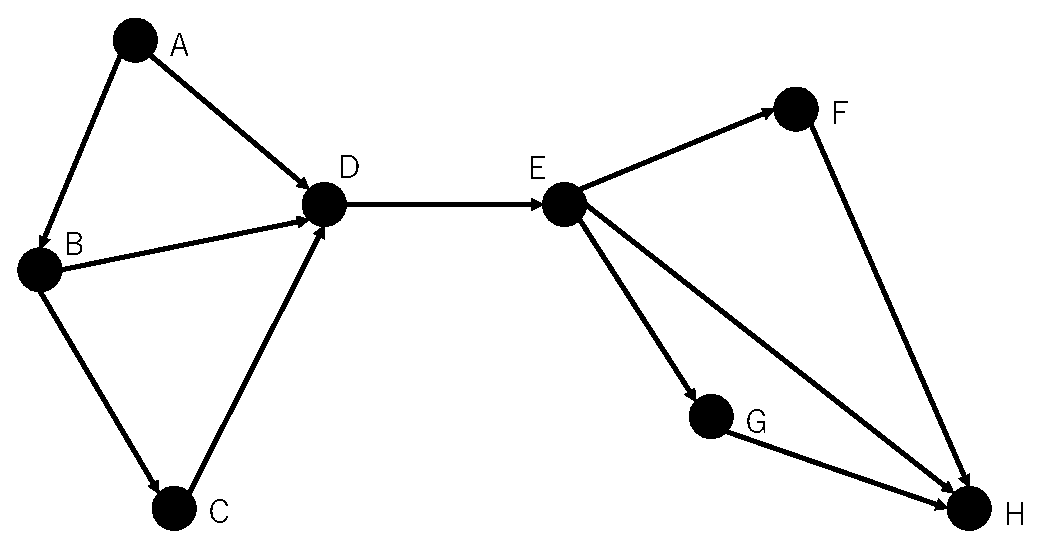
\includegraphics[keepaspectratio,scale=0.5]{fig/2/DAG.eps}
\caption{有向非巡回グラフの例}
\label{fig:DAG}
\end{center}
\end{figure}
有向グラフは頂点と有向辺から構成され,辺は頂点同士をつなぐが,ある頂点 v から出発し辺をたどっても、頂点 v に戻ってこないというものである.
Race logicでは最短・最長経路を探索するために,各パスをにおいて条件に合わせて重み付けを行い,出力時にその重みの総和を見る.
その総和の最小値を見るか最大値を見るかが,最短・最長経路探索にそれぞれ対応している.

重みに遅延時間を選択することによって,各パスを通過する信号毎に出力のタイミングが変わってくる.
信号がRace Logicを用いた回路に入力されてから出力されるまでの遅延時間を計測することが,パスの重みの総和を見ることに等しい.
最短経路検索においては一番早く出力された信号の出力タイミングを,最長経路検索においては一番遅く出力された信号の出力タイミングのみを見る.
つまり,出力のタイミングを競うレースに勝利した信号の出力タイミングのみを見る,ということであり,Race Logicの名前の所以でもある.
出力信号の遅延時間がとある情報を持つ計算結果となる.
例として,図\ref{fig:DAG1}の頂点Aに信号を入力し,
頂点Hから出力されるものを考える.
\begin{figure}[t!]
\begin{center}
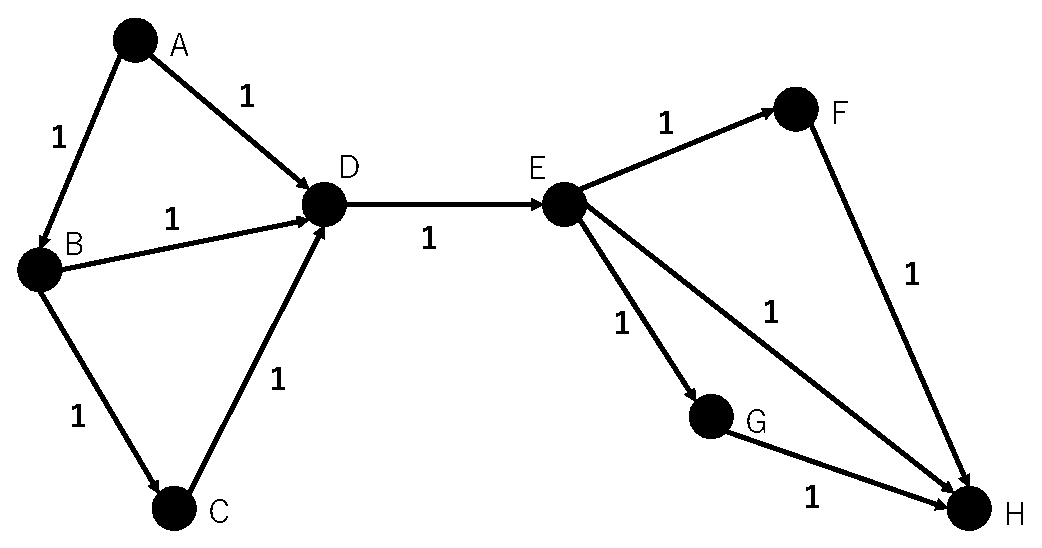
\includegraphics[keepaspectratio,scale=0.5]{fig/2/DAG1.eps}
\caption{Race Logicの例}
\label{fig:DAG1}
\end{center}
\end{figure}
これは図\ref{fig:DAG}の一辺を通過する際の遅延時間を1としたものである.
頂点Aに信号を入力してから頂点Hに至る経路は,
A→D→E→F→G,A→D→E→G→H,A→D→E→H,
A→B→D→E→F→G,A→B→D→E→G→H,A→B→D→E→H,
A→B→C→D→E→F→G,A→B→C→D→E→G→H,A→B→C→D→E→Hの9通り考えられ,
各経路を通った信号の遅延時間はそれぞれ4,4,3,5,5,4,6,6,5である.
よって最短経路はA→D→E→Hであり,一番最初に出力される信号の遅延時間は3である.
一辺の通過の際の遅延時間を1としたので,
一番最初に出力された信号の遅延時間は頂点Aから頂点Hまでの距離を表している.

このように出力信号の遅延時間はとある情報を持っており,
どのような情報を持つかは応用するアプリケーションによって異なる.

\section{配列アラインメント}
生物学の分野において注目されている生物配列(DNAの塩基配列とタンパク質アミノ酸配列) の文字列処理(配列情報解析)
\cite{浅井潔2000配列情報と確立モデル,後藤修1998マルチプルアラインメントは生体高分子情報の交差点}
の中でも,今回は配列アラインメントに焦点を当てる.

DNAやタンパク質はユニットと名付けられた単位の物質が一列に並んだ高分子である.
ここでいうユニットとは,DNAにおいては4種の核酸,タンパク質においては20種類のアミノ酸である.
それぞれのユニットを文字としDNAやタンパク質の配列を単なる文字列だとみなして
処理をしてもある種の本質は失われないという考えに基づき,
文字列処理をすることで生物配列の解析を行なっている.
DNAの塩基配列やタンパク質アミノ酸配列の研究は,
バイオインフォマティクスの最重要課題の一つとして取り組まれてきた.
配列情報解析の重要な対象であるゲノム塩基配列は,
すでに200種類以上が決定されており,さらに多くの解析が進行中であるといわれている
\cite{浅井潔2005バイオインフォマティクス}.

生物配列の文字列処理の中で,DNA配列中に同じ順序で並んでいるユニットのパターンを見つける
配列アラインメントがある\cite{須戸里織2011バイオインフォマティクスゲノム配列から
機能解析へバイオインフォマティクスゲノム配列から機能解析へ}.
アラインメントとは,複数の配列を入力として配列要素の間に最適な対応関係を求める処理である.
配列アラインメントの中には,グローバル配列アラインメントとローカル配列アラインメントというものがある.
グローバル配列アラインメントは,ある2つ以上の配列全体の間でのアラインメントを見つけることであり,
ローカル配列アラインメントは,ある2つ以上の配列の一部分で最も一致度が高い部分でのアラインメントを見つけることである.
配列Pと配列Qのグローバル配列アラインメントとローカル配列アラインメントを例として図\ref{fig:grlc}に示す.
\begin{figure}[t!]
\begin{center}
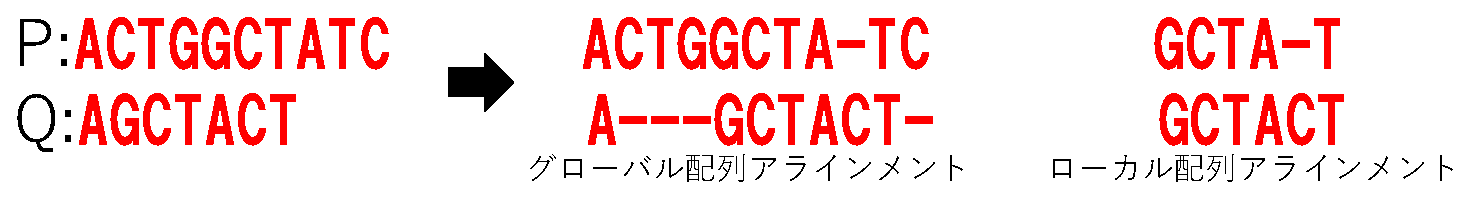
\includegraphics[keepaspectratio,scale=0.5]{fig/2/grlc.eps}
\caption{グローバル配列アラインメントとローカル配列アラインメント}
\label{fig:grlc}
\end{center}
\end{figure}

配列アラインメントには,動的計画法による解法としてNeedleman-Wunschアルゴリズム\cite{needleman1970general}やSmith-Watermanアルゴリズム\cite{smith1981identification}が存在する.
配列アラインメントは生物学において重要な手法であり,
計算機を用いた処理の高速化は従来より多くの研究がなされてきた\cite{須戸里織2011gpu,宗川裕馬2008統合開発環境,sandes2011smith,liu2015accelerating,伊野文彦2007gpu}.

文字列の類似度を知るための典型的な手法は,情報理論に由来する編集距離 (edit distance) である.
編集距離は,一方の文字列をもう一方の文字列に変形するのに必要な手順である一文字の挿入・削除・置換に
それぞれ編集スコアを割り当て,そのスコアの和として定義される.
編集距離の理解を助けるために,長さN = 5の文字列A= "TCGAT"と長さM = 5の文字列B= "GTCAC"を考える.
\begin{figure}[t!]
\begin{center}
\subfigure[]{
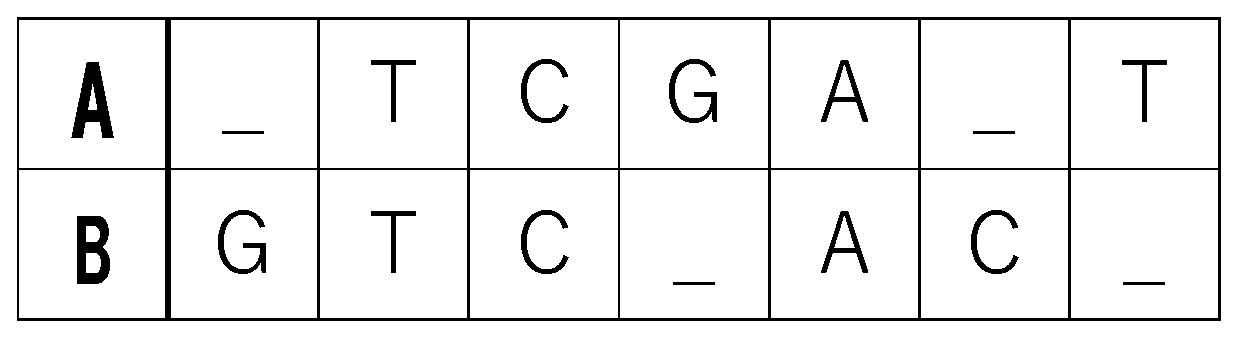
\includegraphics[keepaspectratio, scale=0.25]{fig/2/ed1.eps}
\label{fig:ed1}
 }
\subfigure[]{
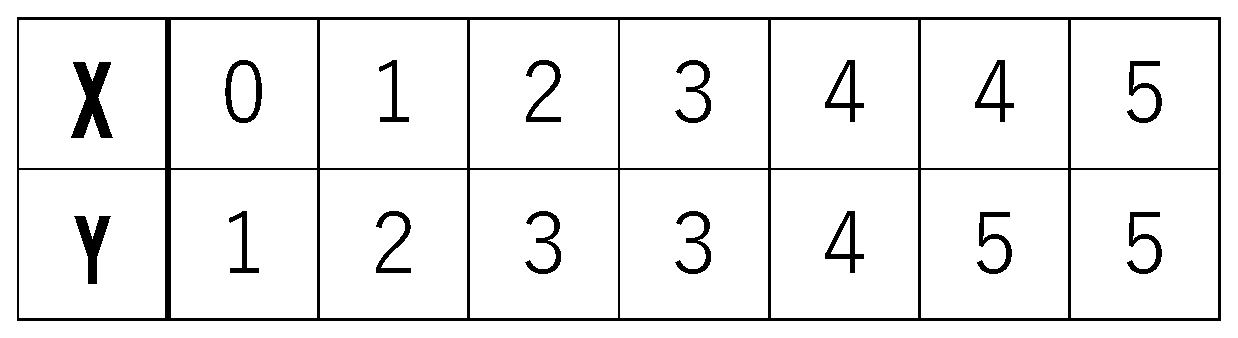
\includegraphics[keepaspectratio, scale=0.25]{fig/2/ed2.eps}
\label{fig:ed2}
 }\\
\subfigure[]{
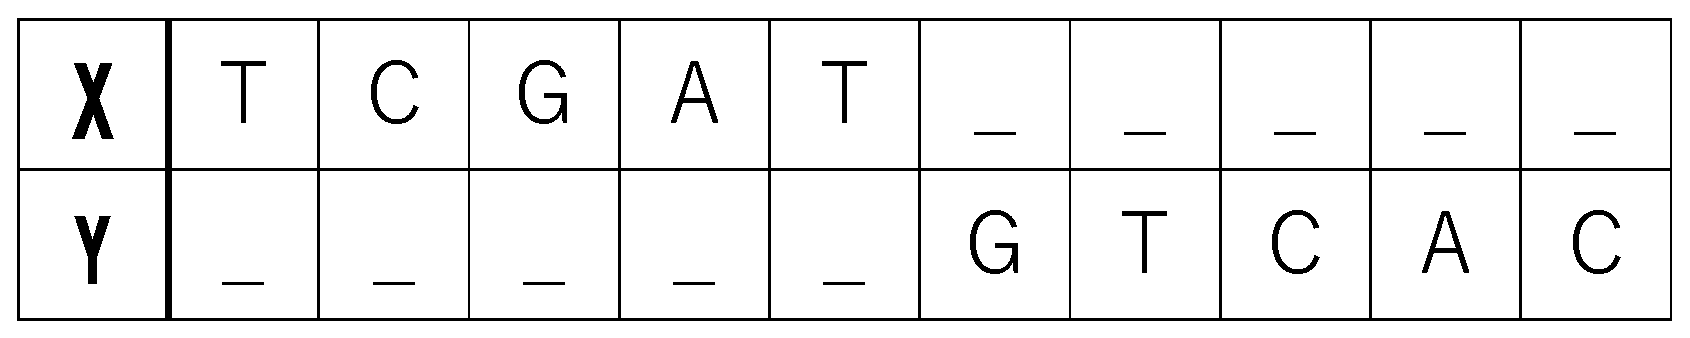
\includegraphics[keepaspectratio, scale=0.25]{fig/2/ed3.eps}
\label{fig:ed3}
 }
\subfigure[]{
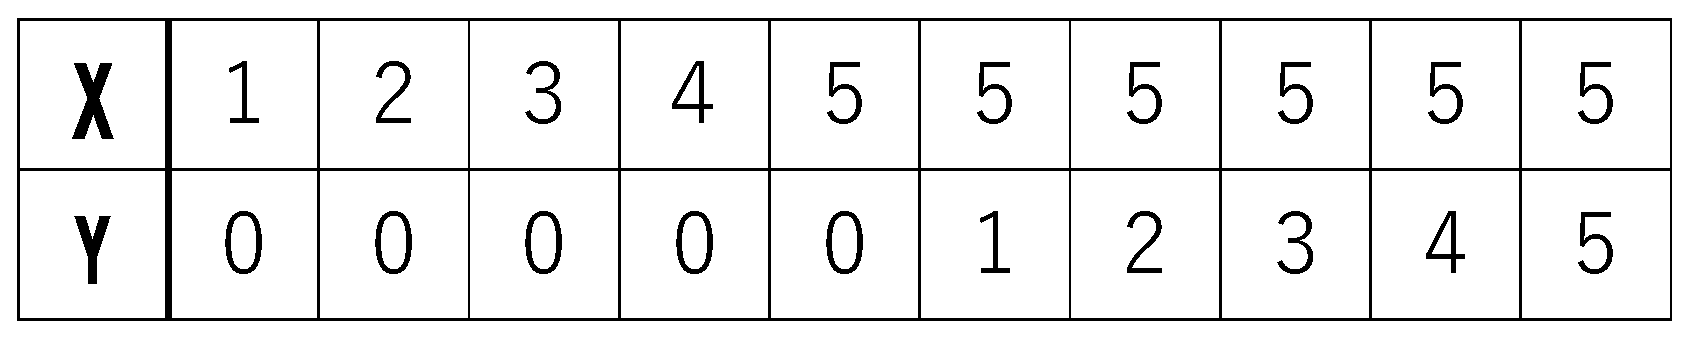
\includegraphics[keepaspectratio, scale=0.25]{fig/2/ed4.eps}
\label{fig:ed4}
 }\\
\subfigure[]{
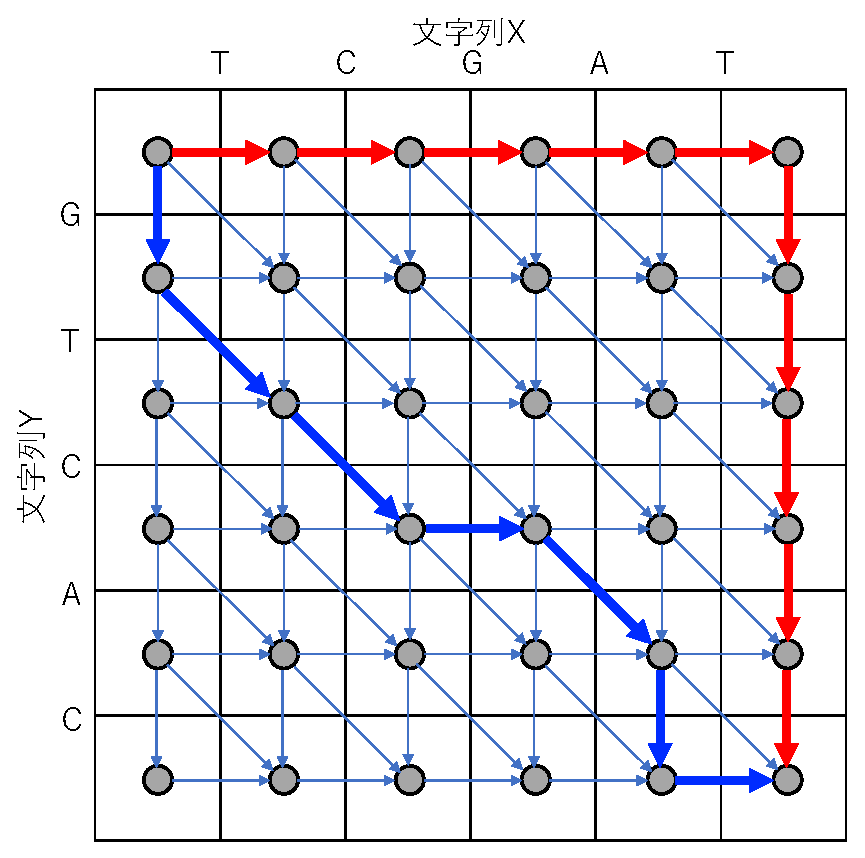
\includegraphics[keepaspectratio, scale=0.5]{fig/2/ed5.eps}
\label{fig:ed5}
 }
\caption{編集距離と編集グラフ}
\label{fig:ed}
\end{center}
\end{figure}
図\ref{fig:ed1}と図\ref{fig:ed3}は,文字列AをBに変換する2つの方法を示している.
上の行のスペースは挿入を表し,下の行のスペースは削除を表す.
両方の行に同じ文字がある列は一致と呼ぶ.
図\ref{fig:ed1}の方法は文字GとTを削除し,GとCを挿入する一方で,
図\ref{fig:ed3}の方法は文字列Aを完全に削除して文字列Bを挿入している.

図\ref{fig:ed2}および図\ref{fig:ed4}は, 2つのアラインメント方法の代替表現である.
任意の位置の数字は,図\ref{fig:ed1}および図\ref{fig:ed3}の方法においてその位置までに存
在する記号の数を示している.
この表示は各列の数値が図\ref{fig:ed5}に示す2次元の編集グラフの座標と考えることができる.
このグラフを編集グラフという.
編集グラフは2つの文字列間において,取りうる限りの配置の
二次元表現である有向非巡回グラフ(DAG)である.
全てのエッジが編集操作に対応していて,垂直の矢印は挿入を,水平の矢印は削除を,斜めの矢印は一致を表している.
任意のアラインメントはこのグラフのパスで表現できる.
例えば、図\ref{fig:ed5}の青と赤の矢印は,それぞれ図\ref{fig:ed1}および図\ref{fig:ed3}に示す2つのアライメントに対応している.

2つの文字列間の編集距離は,動的計画法を用いて計算できる.
動的計画法は小さな部分問題から始めて次第に大きな問題を漸進的に解決し,
各ステップはそれ以前の計算の結果に依存している.
編集グラフ上の各ノードは,部分問題の最適解に対応するスコア,
すなわち最初のノードから自身への最短経路に対応するスコアを計算している.
隣接するノードは,計算が対角線に沿って進むにつれてそれ以前の最適解を利用して
自身のスコアを計算する.
編集グラフ自体は最初のノードから最後のノードまでの経路として,
表現される可能性のあるすべてのアライメントから構成されている.
よって,上記の方法は比較対象の文字列間の最適なアライメントについて
空間全体の検索が保証されている.

任意の2つの文字列が与えられた場合,多数の異なるパスがあり,それぞれが独自のアラインメントを持つ.
ある特定のアライメントの相対的なメリットを決定するために
スコアマトリックスが導入される.
このスコアマトリックスは効果的に編集グラフの各エッジの重みを定義することができる.
スコアマトリックスとはあるユニット間の一致不一致や置換確率から求められる
スコアからなる行列である.
一致・不一致スコアと対数オッズスコアの式を式\ref{eq:mchun}と式\ref{eq:odds}にそれぞれ示す.
\begin{equation}
S(A,B)= \left \{
\begin{array}{l}
\alpha \ \ A = B\\
\beta \ \ A \neq B
\end{array}
\right.
\label{eq:mchun}
\end{equation}
\begin{equation}
S(A,B)= \log \cfrac{q(A,B)}{p(A)p(B)}
\label{eq:odds}
\end{equation}
$ここでq(A,B)は進化上の関係からAとBの対応が生じた確率,
p(A)は偶然にAが生じた確率,p(A)P(B)は偶然にAとBの対応が生じた確率である.$
図\ref{fig:scorematrix}には式\ref{eq:mchun}に具体的な数値を当てはめた場合のスコアマトリックス例を示す.
一般的に,不一致のペナルティは特定の文字のペアにも依存することに注意が必要で
ある.
\begin{figure}[t!]
\begin{center}
\subfigure[最長経路探索に用いられるスコアマトリックス]{
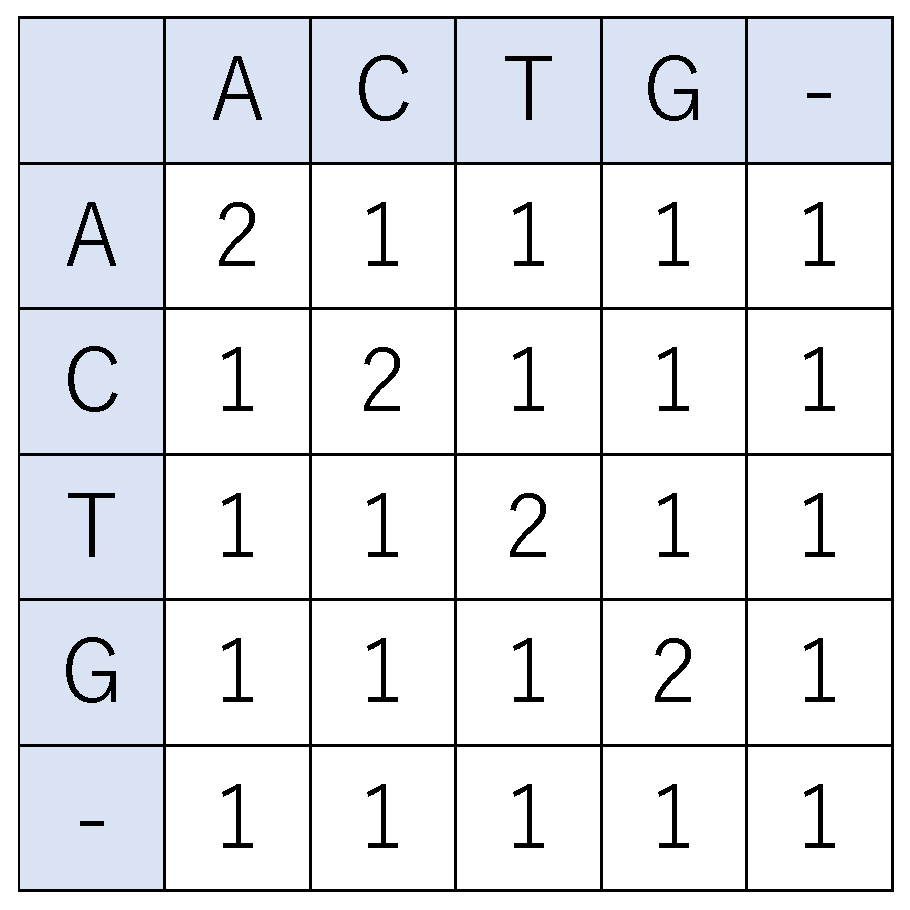
\includegraphics[keepaspectratio,scale=0.5]{fig/2/maxscore_ex.eps}
\label{fig:scorematrixmax}}
\subfigure[最短経路探索に用いられるスコアマトリックス]{
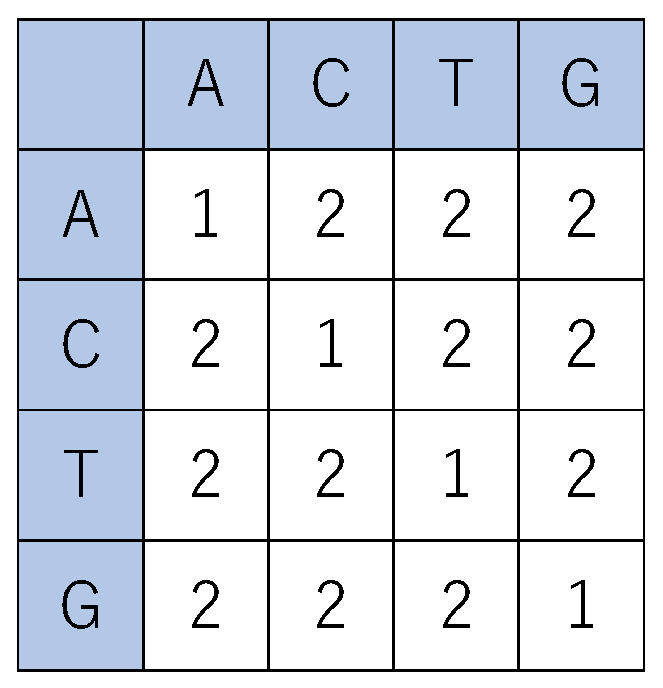
\includegraphics[keepaspectratio,scale=0.5]{fig/2/minscore_ex.eps}
\label{fig:scorematrixmin}}
\caption{スコアマトリックスの例}
\label{fig:scorematrix}
\end{center}
\end{figure}

あるノードにおけるスコアの最大値と最小値を求める関数は
式\ref{eq:maxscore}と式\ref{eq:minscore}のように書ける.
\begin{subequations}
\begin{align}
S_{i,j}= max \left \{
\begin{array}{l}
S_{i-1,j}+\delta(-,P_{j}) \\
S_{i,j-1}+\delta(Q_{i},-) \\
S_{i-1,j-1}+\delta(Q_{i},P_{j})
\end{array}
\right.\label{eq:maxscore} \\
S_{i,j}= min \left \{
\begin{array}{l}
S_{i-1,j}+\delta(-,P_{j}) \\
S_{i,j-1}+\delta(Q_{i},-) \\
S_{i-1,j-1}+\delta(Q_{i},P_{j})
\end{array}
\right.\label{eq:minscore}
\end{align}
\label{eq:minmaxscore}
\end{subequations}
iとjは図\ref{fig:ed5}に示す行と列のインデックスである.

アラインメントのメリットを決定することとはつまり,
図\ref{fig:scorematrixmax}のマトリックスと式\ref{eq:maxscore}を用いて最長経路を探索すること,
または図\ref{fig:scorematrixmin}のマトリックスと式\ref{eq:minscore}を用いて最短経路を探索することと等しい.

\section{CMOSによるRace Logic実装}
本節では,CMOSを用いたRace Logic実装例として,配列アラインメントアクセラレータを説明する.
Race Logicの考えを用いて実装された配列アラインメントアーキテクチャの基本構造を図\ref{fig:racelogicarray}に示す.
このRace Logic Arrayはセルと呼ばれる単位のユニットが繰り返される構造をとっている.
\begin{figure}[t!]
\begin{center}
\subfigure[Race Logicを用いた配列アラインメントアクセラレータの構成]{
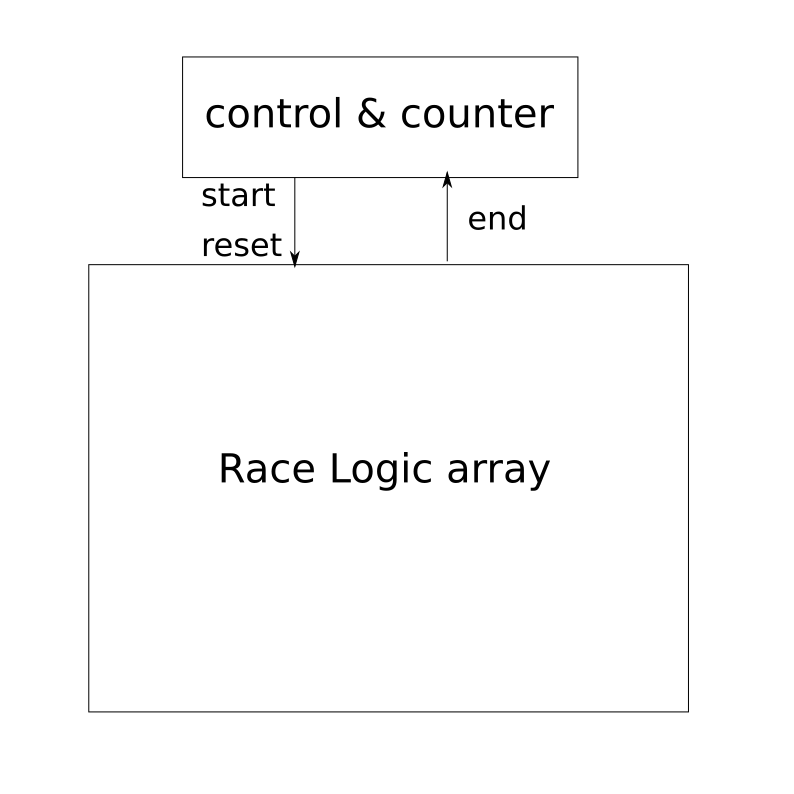
\includegraphics[keepaspectratio,scale=0.3]{fig/2/lightracelogic_1.png}}
\subfigure[Race Logic Arrayの構成]{
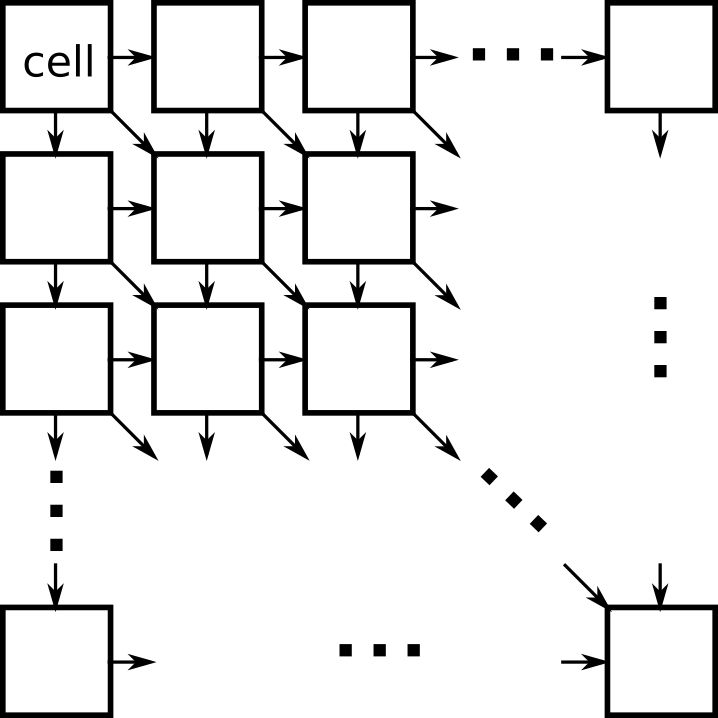
\includegraphics[keepaspectratio,scale=0.3]{fig/2/lightracelogic_2.png}}
\caption{配列アラインメントアクセラレータの基本構造}
\label{fig:racelogicarray}
\end{center}
\end{figure}
図\ref{fig:ed5}に示す編集グラフに対して,Race Logic Arrayが編集グラフ全体に,セルがノードに対応する.
セルは上・斜上・左のセルから信号の入力を受け付ける.
信号が入力された後,設定された条件に合わせて適切な処理をした後に,
次のセルへと信号を出力する.
実装の選択肢として,セルへの信号伝搬をクロックと同期させる同期型と,セルへの信号伝搬をクロックと同期させない非同期型とがある.

最短経路探索を行うことでDNAグローバル配列アラインメントスコアを得る配列アラインメントアクセラレータについて,同期型と非同期型を見ていく.

\begin{itemize}
\item CMOSによる同期型Race Logic実装\\
CMOSで実装された同期型Race Logicのセルの構造を図\ref{fig:CMOSsync}に示す.
\begin{figure}[t!]
\begin{center}
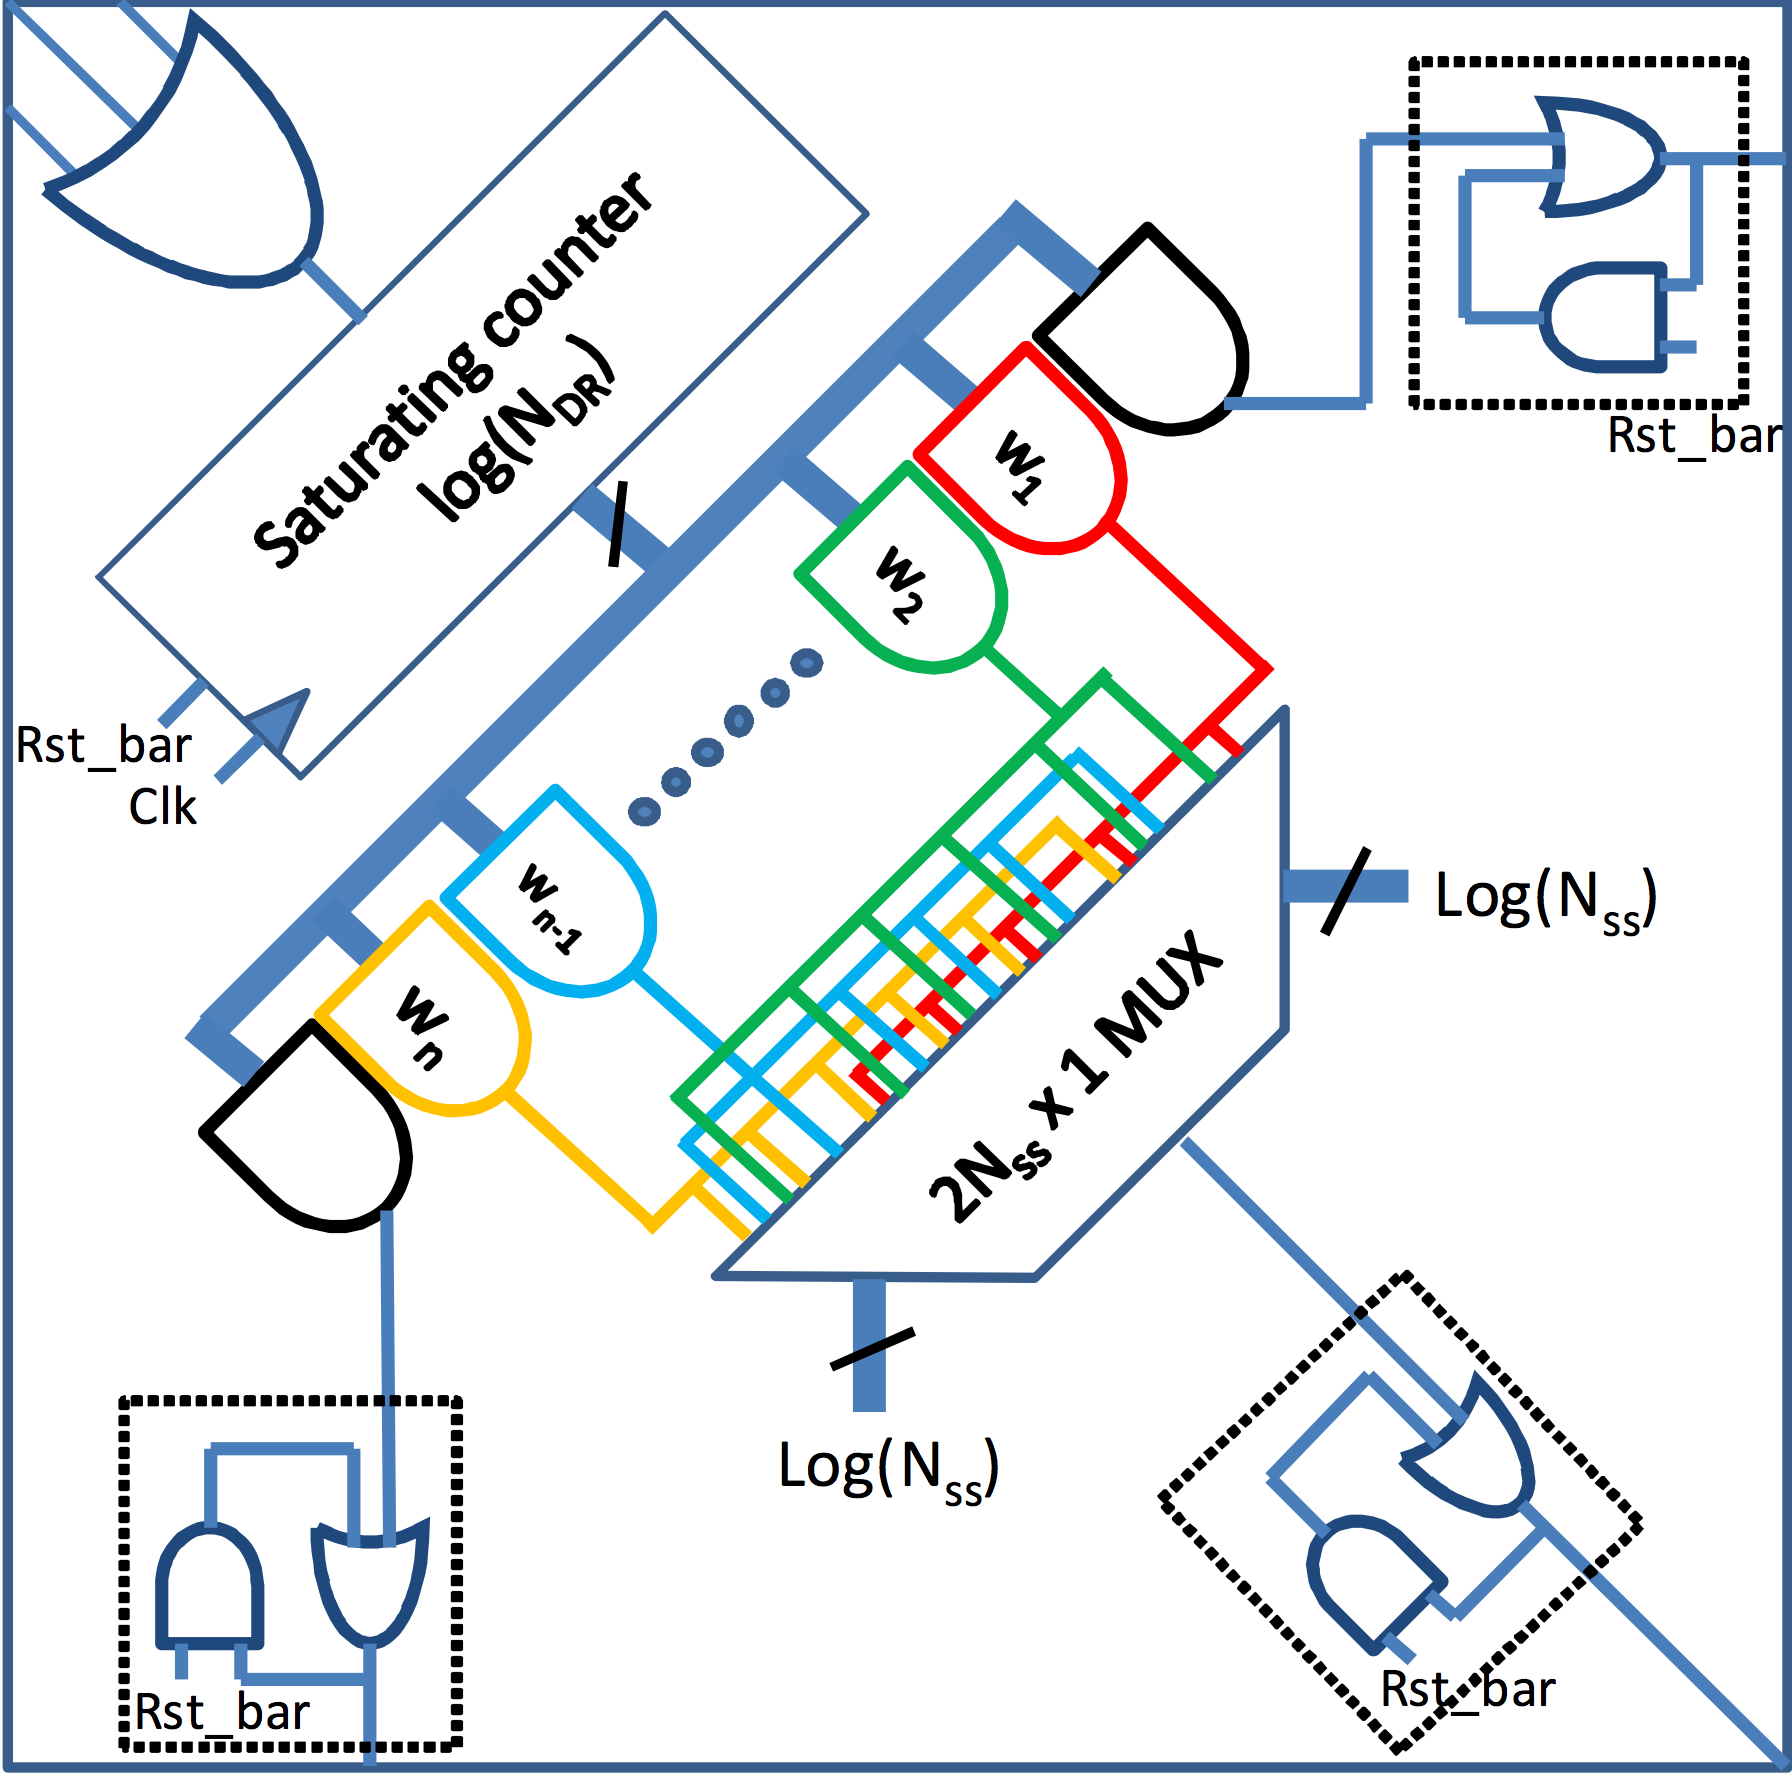
\includegraphics[keepaspectratio,scale=0.3]{fig/2/CMOSsync.png}
\caption{CMOSで実装された同期型Race Logicのセル構造\cite{madhavan2014race}}
\label{fig:CMOSsync}
\end{center}
\end{figure}

ブール値“1”の信号は左・斜上・上のセルのいずれからも入力される.
入力された信号はORゲートを通過して、飽和アップカウンタにおいてNクロックサイクルに0をカウントする.この飽和アップカウンタをクロックと同期させる.
これにより,1つのセルを通過し,右・下のセルへと伝搬する際に1クロックサイクルを要する.
各着色ゲートの出力は,所望の重量に達した時点でトリガーする特定の重量を表しており,アルファベットの符号化を入力とするMUXから所望の重量を選択することができる.
生成される出力信号がパルスではなく固定ブール値“1”であることを確実にするために,到着回路のセットが配置され,各計算の最後にリセットされている.

図\ref{fig:CMOSsync}のセルを繰り返した構造を持つアレイに信号が入力された時から出力信号を得るまでのクロック数をカウントするカウンタがアレイ外部に存在する.
このカウンタが計測した値が最短経路をパスした時のクロック数となる.

\item CMOSによる非同期型Race Logic実装\\
CMOSで実装された非同期型Race Logicのセルの構造を図\ref{fig:CMOSasync}に示す.
\begin{figure}[t!]
\begin{center}
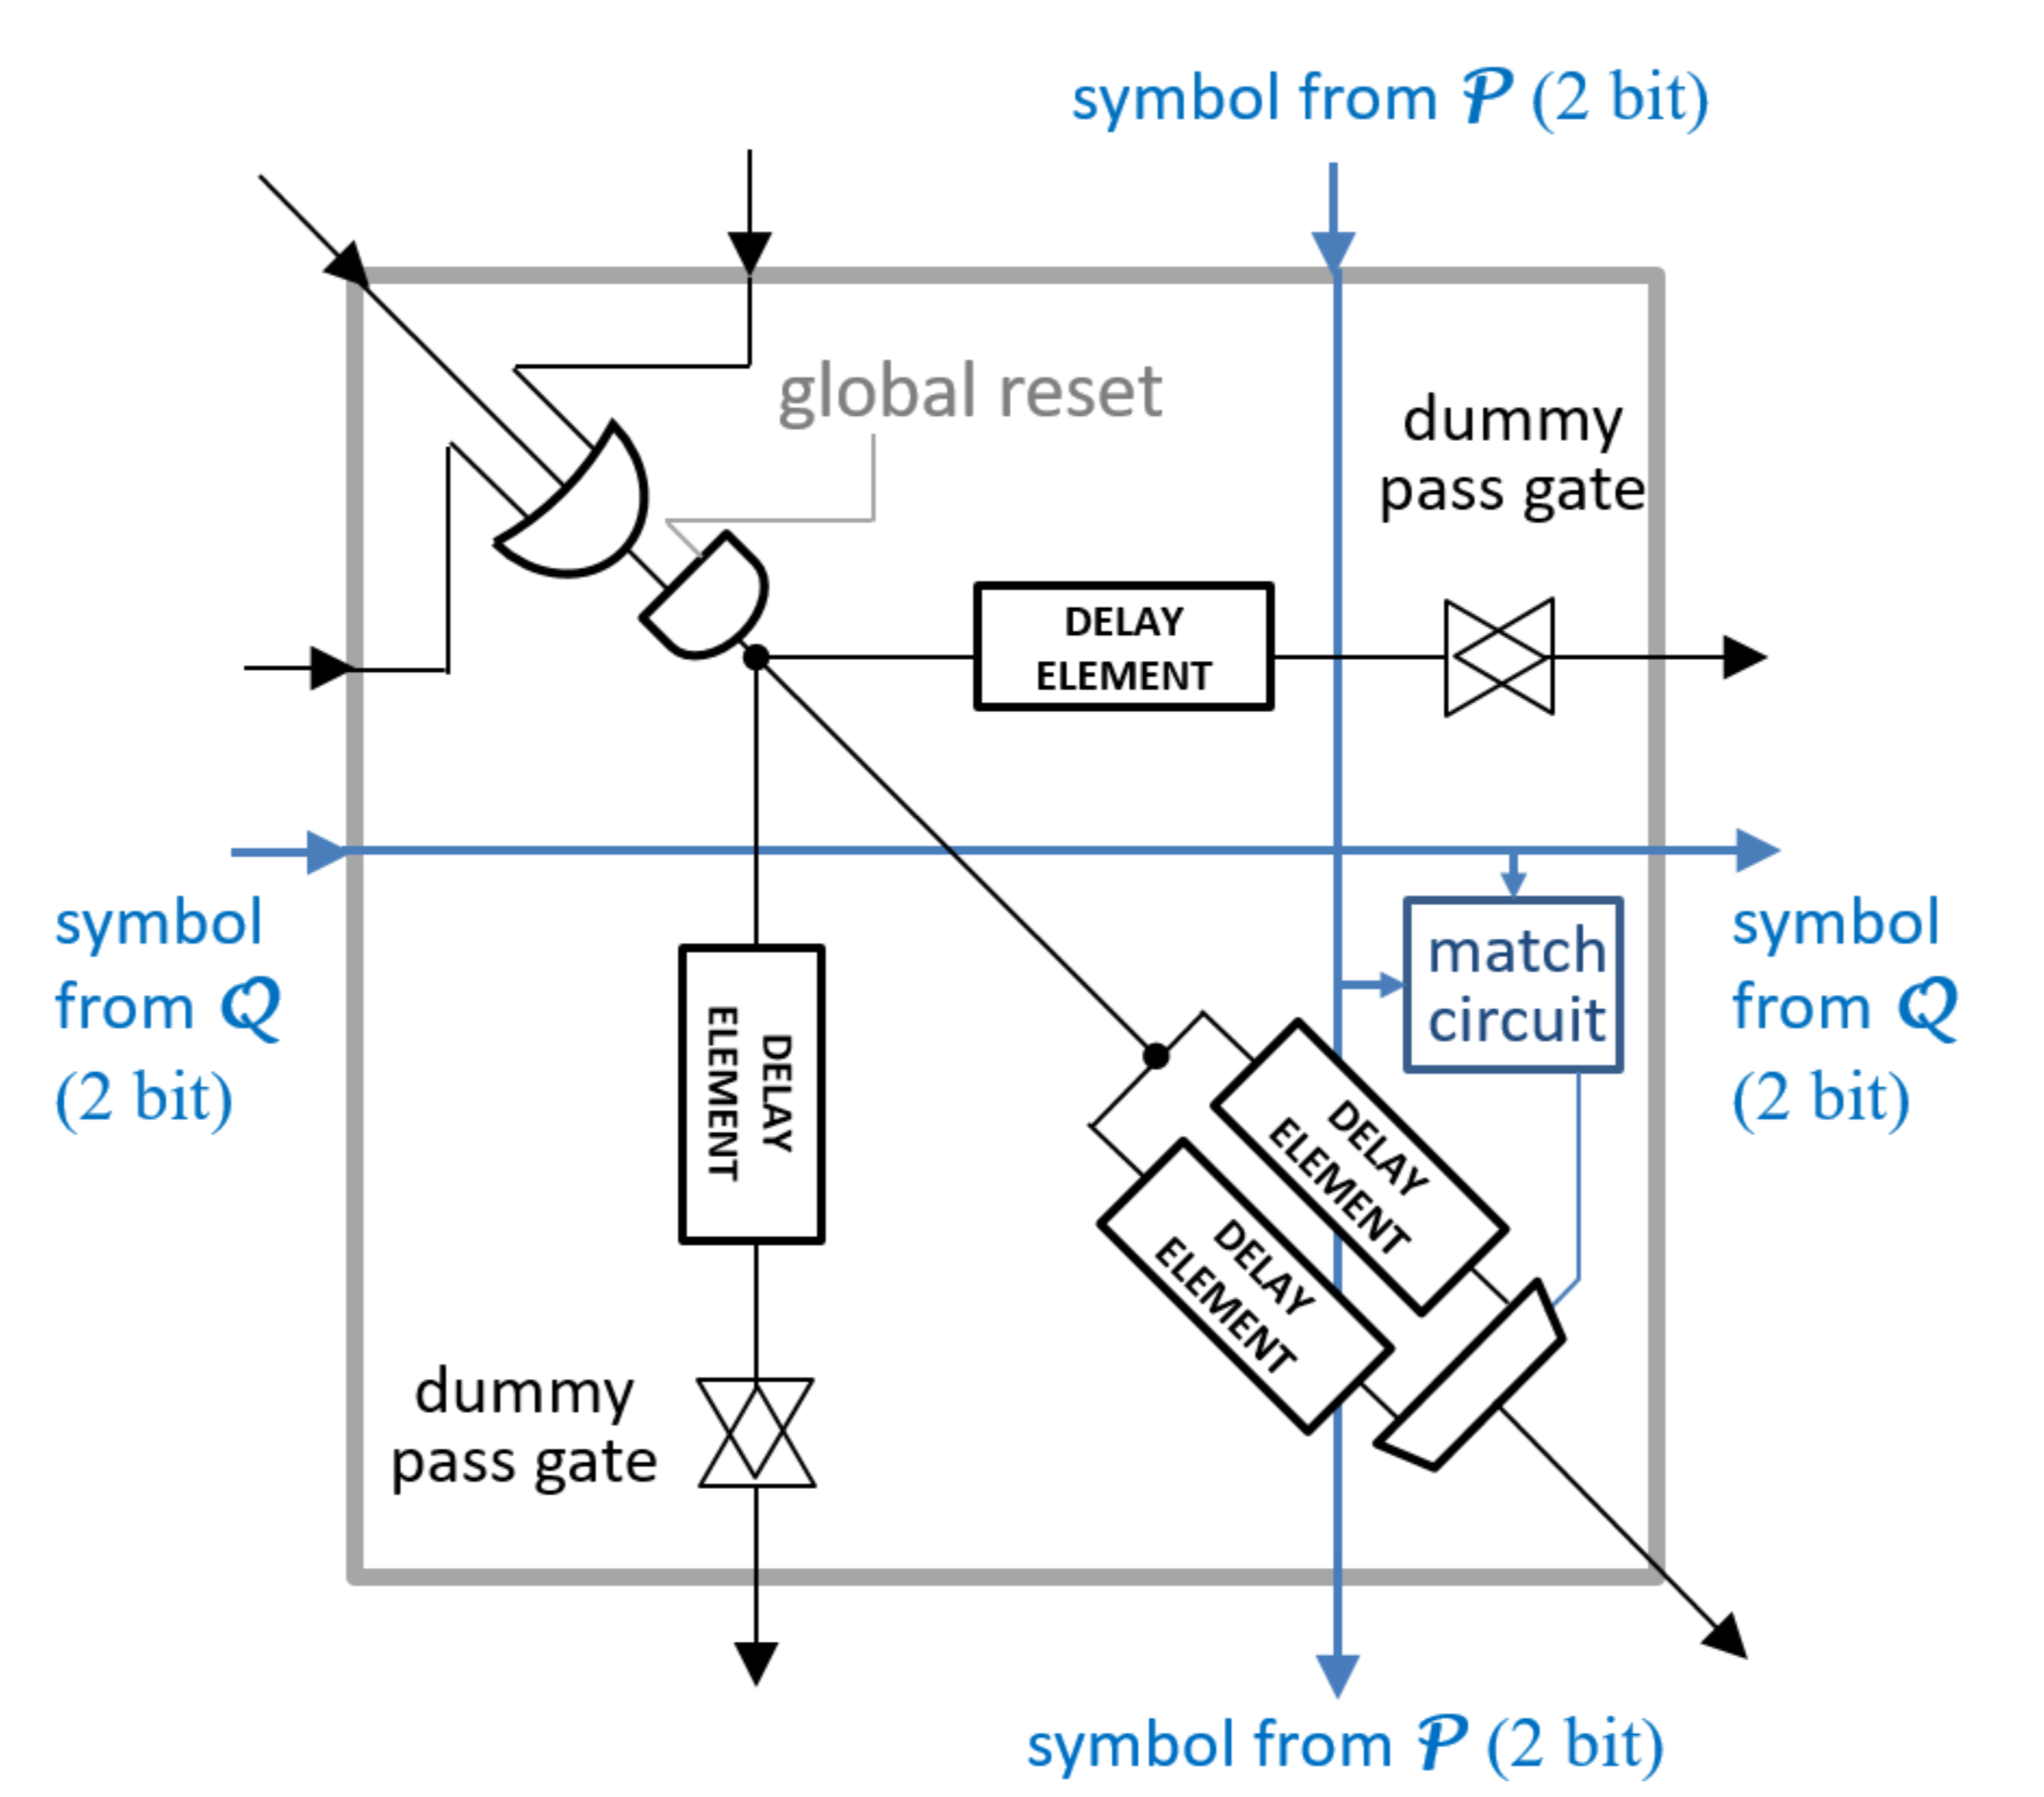
\includegraphics[keepaspectratio,scale=0.3]{fig/2/CMOSasync.png}
\caption{CMOSで実装された非同期型Race Logicのセル構造\cite{madhavan20174}}
\label{fig:CMOSasync}
\end{center}
\end{figure}

ブール値“1”の信号は左・斜上・上のセルのいずれからも入力される.
入力された信号はORゲート,リセットのためのANDゲートを通過する.
アレイのリセットのタイミングは,全ての遅延素子が確実にリセットされるように外部から調整される.
ANDゲートを通過後に次のセルへの伝搬に向けて分けられ,それぞれの経路で遅延素子を通過する.
各着色した経路では遅延素子によって起こる遅延に変化をつけている.
同期型と同様,アルファベットの符号化を入力とするMUXから所望の遅延を選択することができる.
ダミーのパスゲートは,全ての遅延経路に亘って同様の遅延を保証するために斜下へのパス以外に追加されている.

図\ref{fig:CMOSasync}のセルを繰り返した構造を持つアレイに信号が入力された時から出力信号を得るまでの遅延時間をカウントするカウンタがアレイ外部に存在する.
\end{itemize}
上記の回路については,シミュレーションをもってその有効性が明らかにされ,
性能・面積・消費電力密度などが報告されている.

\begin{comment}
\section{解決すべき課題}
これまでRace Logicの基本原理を述べ,CMOSによるRace Logic実装を見てきた.
CMOSによって実装されたRace Logicについては,その有効性が明らかにされ,
性能・面積・消費電力密度なども報告されている.
しかしながら,Race Logicの設計選択肢はCMOSだけに限られず,
CMOS以外の素子を選択した場合の可能性については明らかになっていない.

そこでRace Logicの更なる高性能化を目的とし,
本論文ではナノフォトニック・デバイスによる実装に焦点を当てる.
\end{comment}


\chapter{ナノフォトニック・デバイスを用いたレースロジック実装の提案}
本章では,本提案のナノフォトニック・デバイスを用いたレースロジック(以下,光レースロジック)アレイを理解する上で必要な光デバイスに関する基本事項を説明し,光レースロジック実装について述べる.

\section{光デバイスについて}
本節では,まず光デバイスの特徴と代表的な光素子,ナノフォトニクスについて説明する.
その後,光デバイスとレースロジックの親和性について述べる.

\subsection{光デバイスの特徴}
以下に光デバイスの特徴をまとめ,詳細を説明する.
光デバイスは光が信号を伝搬する素子全般のことを指す.
一方,本論文では電気デバイスとは電気が信号を伝搬するCMOSトランジスタを指すものと定義する.
\begin{itemize}
\item デバイスサイズ\\
現状,光デバイスのゲート長は$cm$〜$mm$オーダーのスケールである.後述するナノフォトニクスを用いたとしても,そのスケールのオーダーは$\mu m$である.
\item 信号の周波数帯域\\
光デバイスにおいて,信号の伝搬は光信号が通過するか否かで行われる.電気デバイスのように時定数によって周波数帯域が制限されることがない.よって,その周波数帯域は広帯域であると言える.
\item データの蓄積\\
電気デバイスは,電荷を貯めることでデータを保持できる.光デバイスは光を留めておくことが難しいため,データの蓄積は困難である.電気デバイスの方が,光デバイスよりもデータの蓄積が容易であると言える.
\begin{comment}
\item スループット\\
データ処理やネットワークにおいてのスループットについて述べる.
スループットとは単位時間あたりの処理量や処理可能なデータ量のことである.
光信号は多重性と呼ばれる複数の異なる周波数を多重して送る事ができる性質を持つ.
光デバイスは光信号の広帯域性や,波長多重,位相多重と言った多重性を利用して,
伝搬信号自体の情報量を増加させることで,転送データ量を向上させることが可能である.
\item レイテンシ\\
\end{comment}
\end{itemize}

電気デバイスはデバイスの小型化が可能という特徴から集積度を上げることが可能である.
それに比べ,現状では光デバイスはその小型化に向いておらず,集積度を上げることが困難であった.
よって演算には電気デバイスが用いられてきた.
一方,光デバイスは伝搬信号の情報量が大きく,信号の移動速度も速いという特徴から通信に使われてきた.

\subsection{光素子の説明}
本項では,代表的な光素子について説明する.その説明にあたり,語句を定義する.
\begin{itemize}
\item 光伝搬信号\\
光デバイスおよび,そのデバイスを用いて構成した回路において,情報を伝搬する光信号を指す.
\item 光伝搬入力信号および光伝搬出力信号\\
光デバイスおよび,そのデバイスを用いて構成した回路において,入力される光伝搬信号を光伝搬入力信号,出力される光伝搬信号を光伝搬出力信号と呼ぶ.光入力信号および光出力信号と略す.
\item 光伝搬入力信号強度および光伝搬出力信号強度\\
光伝搬入力信号および光伝搬出力信号の信号強度を指す.単位は[W]である.光入力信号強度および光出力信号強度と略す.
\item 光制御信号\\
光デバイスを制御するための光信号を指す.
\item 光制御信号強度\\
光制御信号の信号強度を指す.単位は[W]である.
\item 電気制御信号\\
光デバイスを制御するための電気信号を指す.
\item 電気制御信号強度\\
電気制御信号の信号強度を指す.単位は[V]である.
\end{itemize}

\subsubsection{光スイッチ}
光スイッチとは,オン動作およびオフ動作によって光伝搬信号を通過させるか
否かを制御する光デバイスである.
光スイッチの性能指標としてよく用いられるのが,
漏れ率,透過率及び消光比である.
\begin{figure}[t!]
\begin{center}
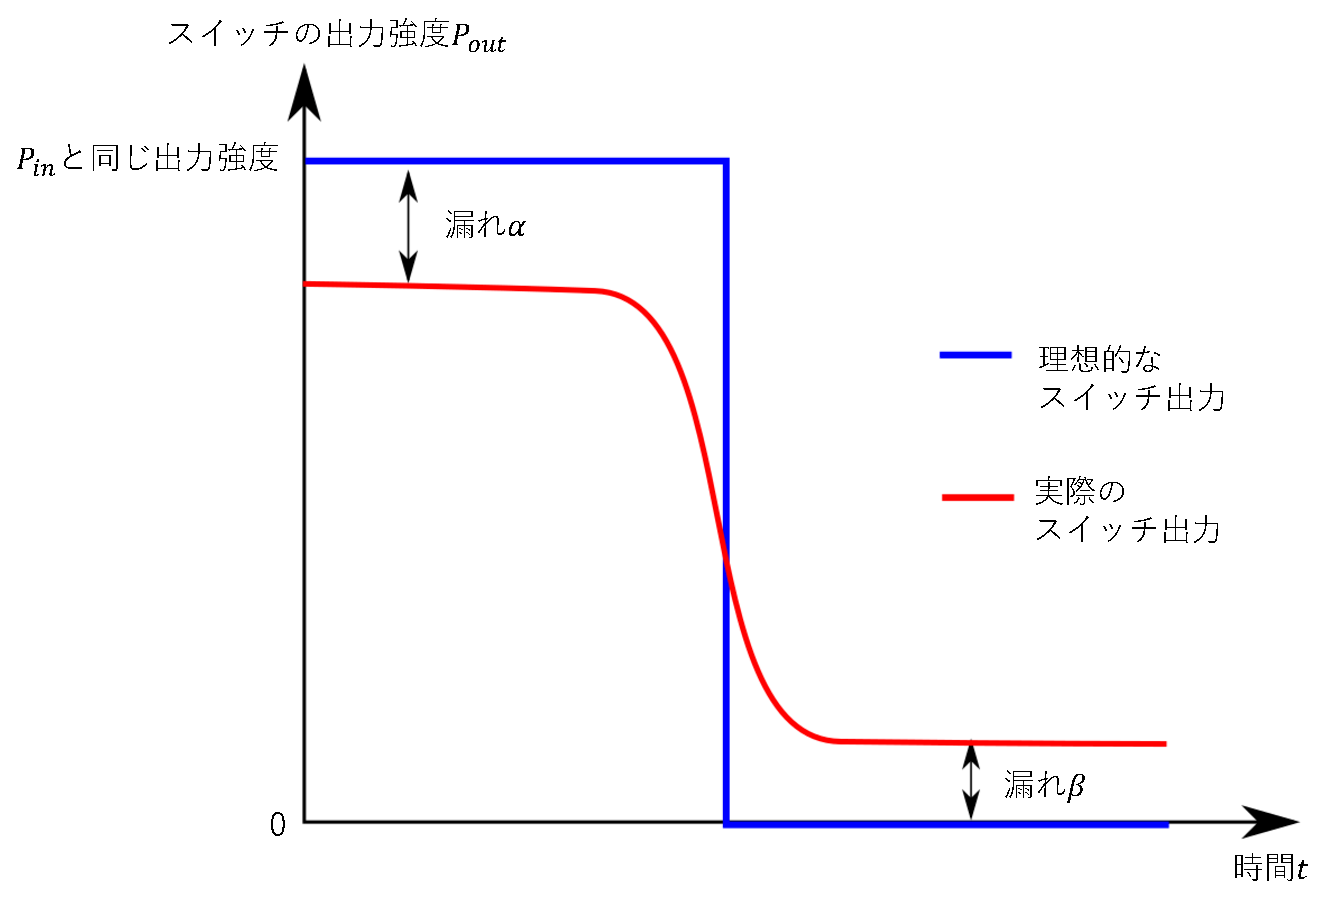
\includegraphics[keepaspectratio,scale=0.5]{fig/3/swichout.eps}
\caption{光スイッチの光入力信号強度と光出力信号強度}
\label{fig:swichout}
\end{center}
\end{figure}
光スイッチへの光入力信号強度を$P_{in}$,光出力信号強度を$P_{out}$とした場合の,
光入力信号強度と光出力信号強度の関係を図 \ref{fig:swichout}に示す.
図の縦軸は光出力信号強度,横軸は時間を表している.
理想的なスイッチでは,光伝搬信号の漏れが無いため光出力信号強度は図の青線に示す関係を取る.
しかしながら,実際にはオン動作とオフ動作どちらの場合でも光伝搬信号の漏れがあるため,
光出力信号強度は図の赤線に示す関係を取る.以下にそれぞれの性能指標の定義を示す.
\begin{itemize}
\item 漏れ率,透過率\\
漏れ率とは,スイッチがオン動作とオフ動作の際,
それぞれどの程度の光伝搬信号が漏れるかということを表す指標である.
図 \ref{fig:swichout}に示す$\alpha $は,
スイッチがオン動作の際にスイッチから回路外へ光伝搬信号がどの程度漏れ出すかを表す漏れ率である.
また,スイッチがオン動作の際にどの程度の光伝搬信号を透過させられるかを表す指標を透過率と呼び,
漏れ率$\alpha$を用いて表すと$1- \alpha$となる.
光スイッチへの光入力信号強度を$P_{in}$,オン動作時の光出力信号強度を
$P_{1out}$とすると,$\frac{P_{1out}}{P_{in}}=1- \alpha$である.
図 \ref{fig:swichout}に示す$\beta $は,スイッチがオフ動作の際に光伝搬信号を遮断しきれずに,
どの程度出力へ漏れ出すかを表す漏れ率である.
光スイッチへの光入力信号強度を$P_{in}$,
オフ動作をする際の光出力信号強度を$P_{0out}$とすると,
$\frac{P_{0out}}{P_{in}}=\beta$である.
$\alpha $,$ \beta $の値が小さいほどスイッチの性能が高いと言える.
\item 消光比\\
消光比とは,スイッチの光出力信号が1と0の場合の光出力信号強度比である.
透過率$1- \alpha$および漏れ率$\beta $用いると,
式~\eqref{eq:syoukouhi}で表される.
\begin{equation}
消光比= \frac{1- \alpha}{\beta}
\label{eq:syoukouhi}
\end{equation}
\end{itemize}
%式~\eqref{eq:syoukouhi}および式~\eqref{eq:oma}から,

消光比は,透過率および漏れ率を用いて議論することが可能であるとわかる.
よって本論文では透過率,漏れ率に着目し,これらをスイッチ性能として議論する.

\subsubsection{受光器}
光の素粒子は一般に光子(フォトン)と呼ばれる.
全ての粒子が波動性を持つことを,粒子と波動の二重性と言う.
光子も粒子性と波動性の2つの性質を持つ\cite{大津}.
光子のエネルギーは光の周波数(波長)で決定する.
\begin{equation}
E = h \nu \label{eq:hikarienergy}
\end{equation}
$Eは光子のエネルギー,hはプランク定数,\nu$は光の周波数である.
光の強度は光子の数によって決定する.

物質中の電子のエネルギーは,取り得るエネルギー準位が限定されている.
そのエネルギー準位は帯構造を取り,図\ref{fig:eg}に示すようにそれぞれ伝導帯,禁制帯,価電子帯と呼ばれる.
伝導帯とは,電子が占めているエネルギー帯のうち最も高いエネルギー準位を示すエネルギー帯である.
この伝導帯は電子が充填されておらず,このエネルギー帯に存在する電子は自由電子として振る舞う.
価電子帯は価電子によって充填されたエネルギー帯である.禁制帯とは電子が存在できないエネルギー帯である.
この禁制帯の幅が図\ref{fig:eg}に示すEgであり,エネルギーギャップと呼ばれる.
半導体物質において,エネルギーギャップを超えるのに十分なエネルギーを持った光子1つが入射した際に,自由電子と正孔のペア1つを生成する.
この現象を{\bf 吸収}という.光子のエネルギーはその光の周波数で決まるため,エネルギーギャップの大きさに対応した周波数がある.
逆の現象が,{\bf 放出}である.これは,自由電子と正孔が再結合した際に,そのエネルギーギャップ$Eg=h \nu$に相当するエネルギーを持つ光子を放出する現象である.
図\ref{fig:kyusyuhosya}に吸収と放出の様子を示す.
図\ref{fig:kyusyuhosya}(a)におけるエネルギーギャップが,緑の光の光子の持つエネルギーと等しいとする.
この際,緑の光を入射すると電子正孔対が生成される.
しかしながら,赤の光は緑の光よりも周波数が小さいため,光子のエネルギーが緑の光と比べて小さい.
よって赤の光を入射しても電子は伝導帯へと励起することができず,電子正孔対は生成されない.
\begin{figure}[t!]
\begin{center}
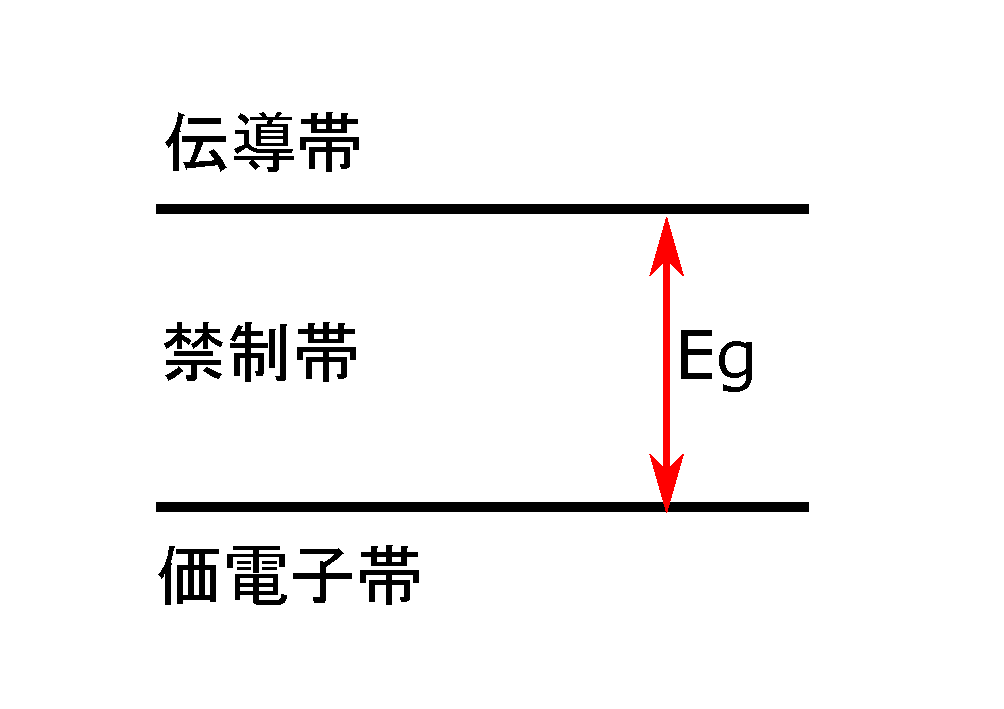
\includegraphics[keepaspectratio,scale=0.4]{fig/3/Eg.pdf}
\caption{半導体のエネルギーバンド図}
\label{fig:eg}
\end{center}
\end{figure}
\begin{figure}[t!]
\begin{center}
\subfigure[吸収]{
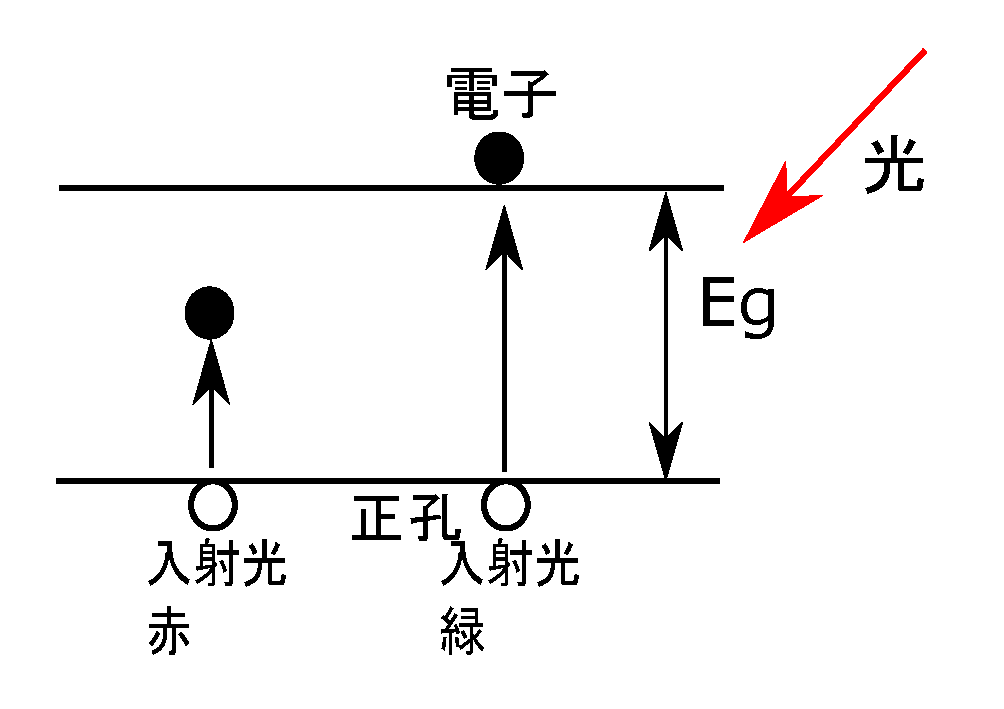
\includegraphics[keepaspectratio,scale=0.4]{fig/3/kyusyu.pdf}}
\subfigure[放出]{
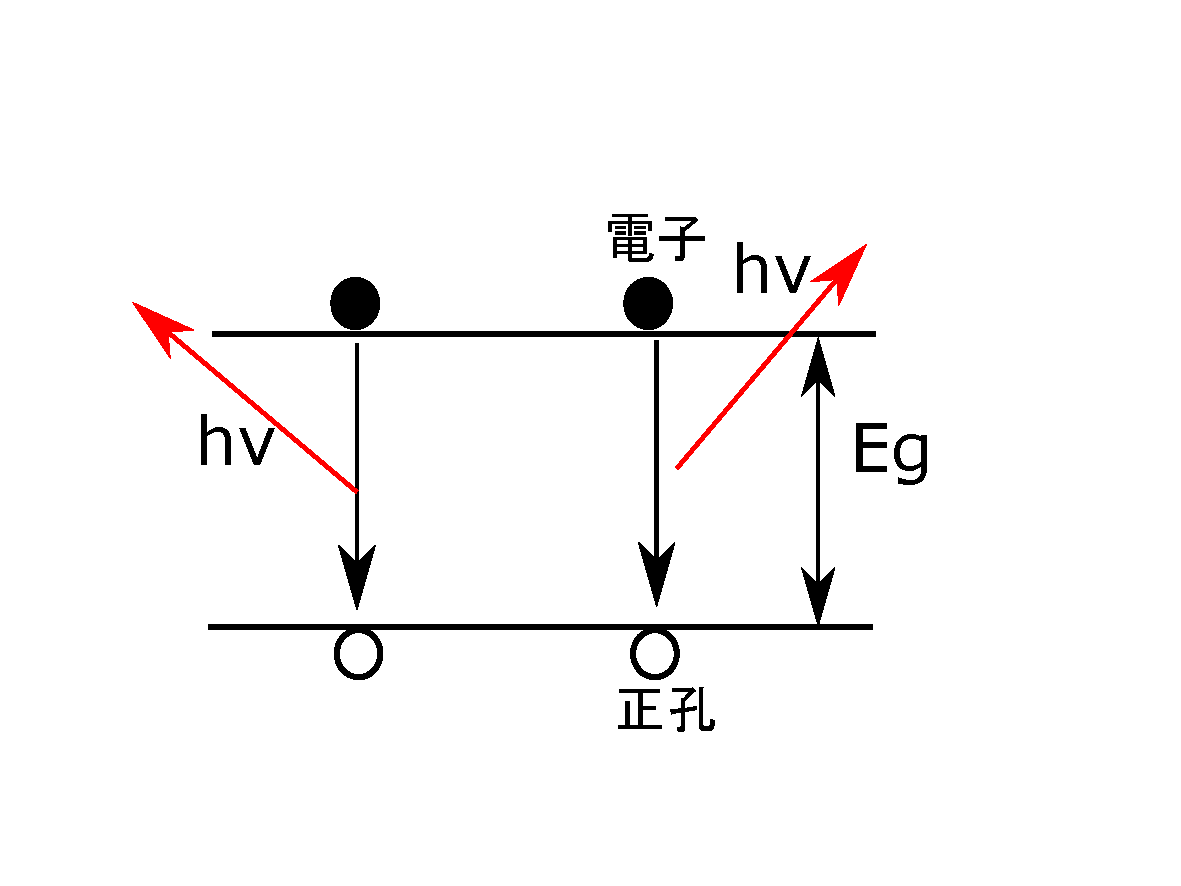
\includegraphics[keepaspectratio,scale=0.4]{fig/3/hosya.pdf}}
\caption{光の吸収と放出}
\label{fig:kyusyuhosya}
\end{center}
\end{figure}
受光器であるフォトダイオードはこの吸収の現象を利用して光を検出する.

フォトダイオードはp型半導体と真性半導体とn型半導体を接合したpin接合という構造を持ち,
空乏層で発生した電子や正孔が移動することで電流が流れる.
この電流のことを光電流と呼ぶ.
流れる光電流の大きさは光の強度に比例する.
図\ref{fig:photo}に受光器のエネルギーバンド図を示す.
\begin{figure}[t!]
\begin{center}
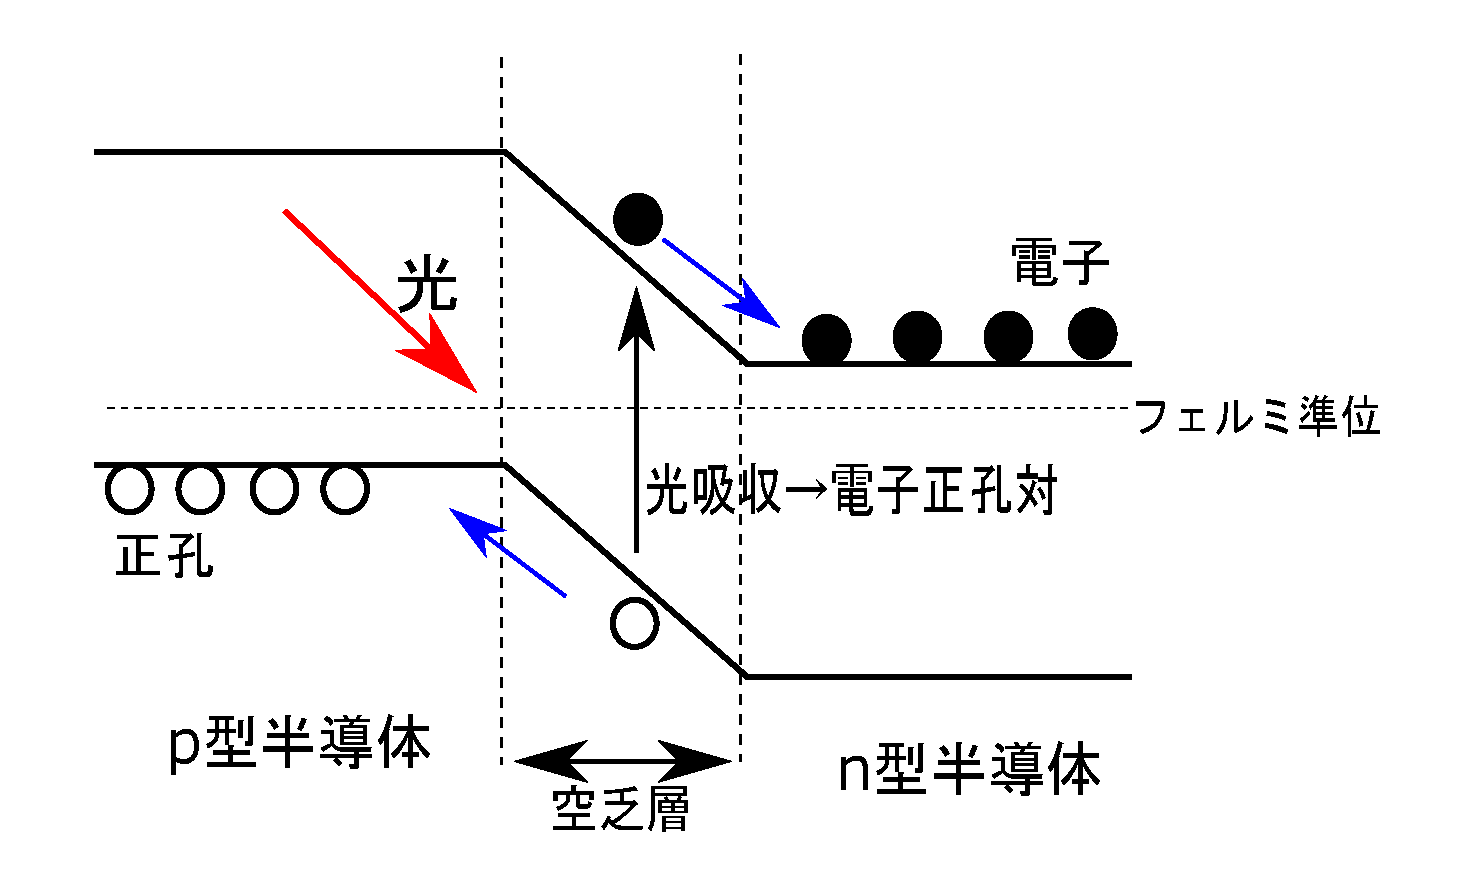
\includegraphics[keepaspectratio,scale=0.4]{fig/3/photodiode.pdf}
\caption{受光器のエネルギーバンド図}
\label{fig:photo}
\end{center}
\end{figure}

受光器の性能は受光感度として表される.
受光感度は,光入力信号強度を[$W$],光電流を[$A$]で表した場合,
両者の比で表される.
受光感度は式~\eqref{eq:jyukoukando}で表される.
式~\eqref{eq:jyukoukando} によって導かれる値が1に近い程,感度の良い受光器であることを示す.
\begin{equation}
受光感度 = \frac{A}{W}
\label{eq:jyukoukando}
\end{equation}
もう一つ重要な性能指標が受光器の最小受光感度である.最小受光感度とは,受光器が検出可能な最小の信号強度のことである.

\subsubsection{光カプラ}
光カプラとは,1つの入力端子に入射した光伝搬信号を複数の出力端子に出射する分岐・分配機能と
複数の入力端子に入射した光伝搬信号を1つの出力端子に出射する結合機能を持つデバイスである.
光分岐結合器,光分岐挿入器とも呼ばれる.
光カプラの分類を図\ref{fig:lcoup}に示す.
4端子で2入力2出力または3入力1出力のものが光方向性結合器(図\ref{fig:lcoup1}),
1入力N出力のものが光分配器もしくは光分岐器(図\ref{fig:lcoup2}),
N入力1出力のものが光結合器(図\ref{fig:lcoup3}),
N入力N出力のものが光スターカプラ(図\ref{fig:lcoup4})と呼ばれている.
光スターカプラの中には透過型と反射型という分類が存在する.
光結合器の多くが入出力端子を逆にすることで光分配器としても使うことができる\cite{ハンドブック}.
また,光の結合・分配の際には損失が発生する.
\begin{figure}[t!]
\begin{center}
\subfigure[光方向性結合器:2入力2出力]{
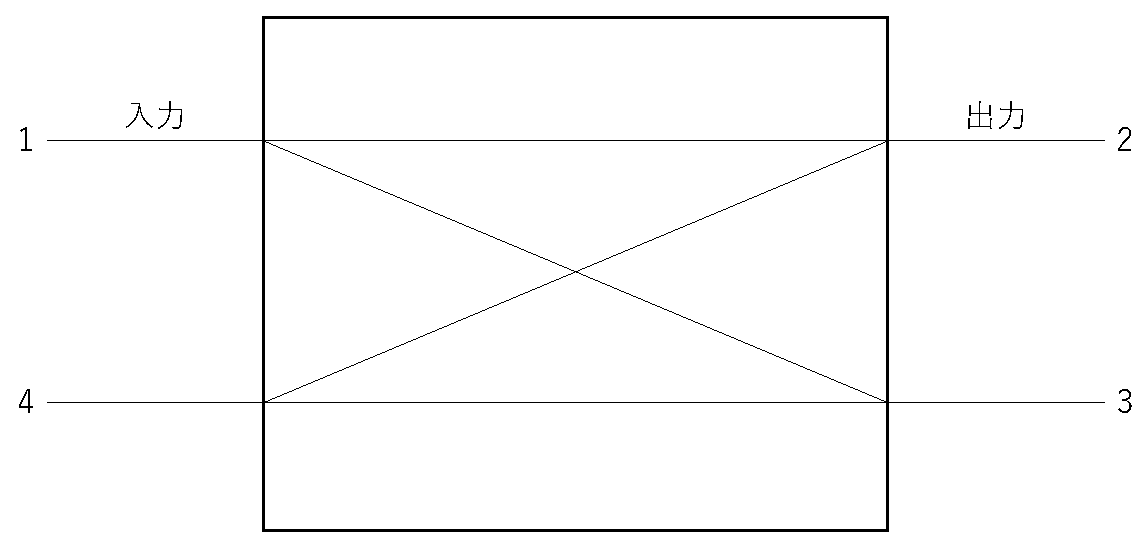
\includegraphics[keepaspectratio, scale=0.4]{fig/3/lcoup1.eps}
\label{fig:lcoup1}
}
\subfigure[光分配器:1入力N出力]{
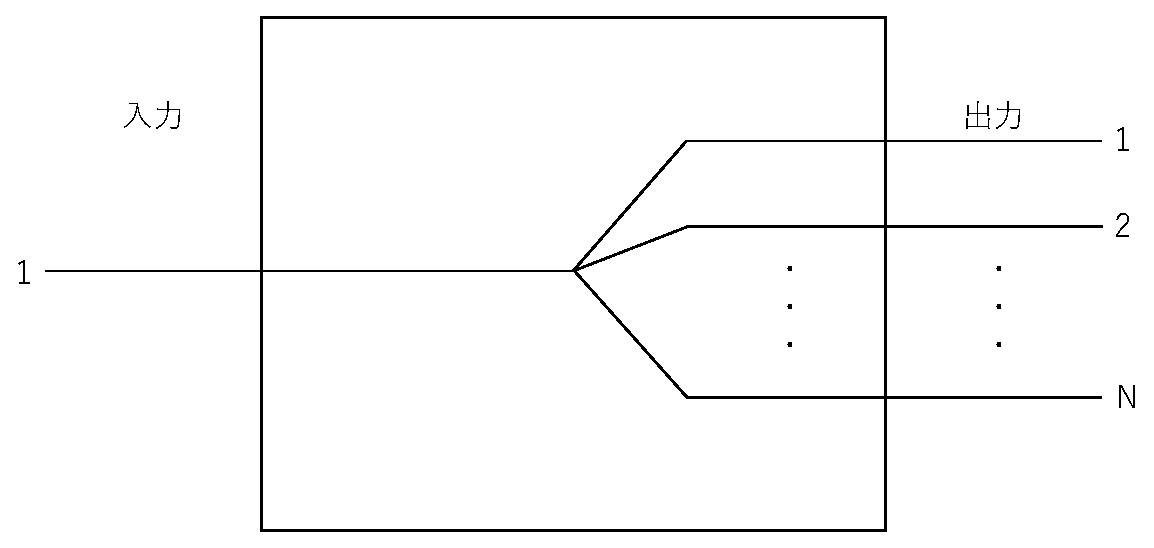
\includegraphics[keepaspectratio, scale=0.4]{fig/3/lcoup2.eps}
\label{fig:lcoup2}
}\\
\subfigure[光結合器:N入力1出力]{
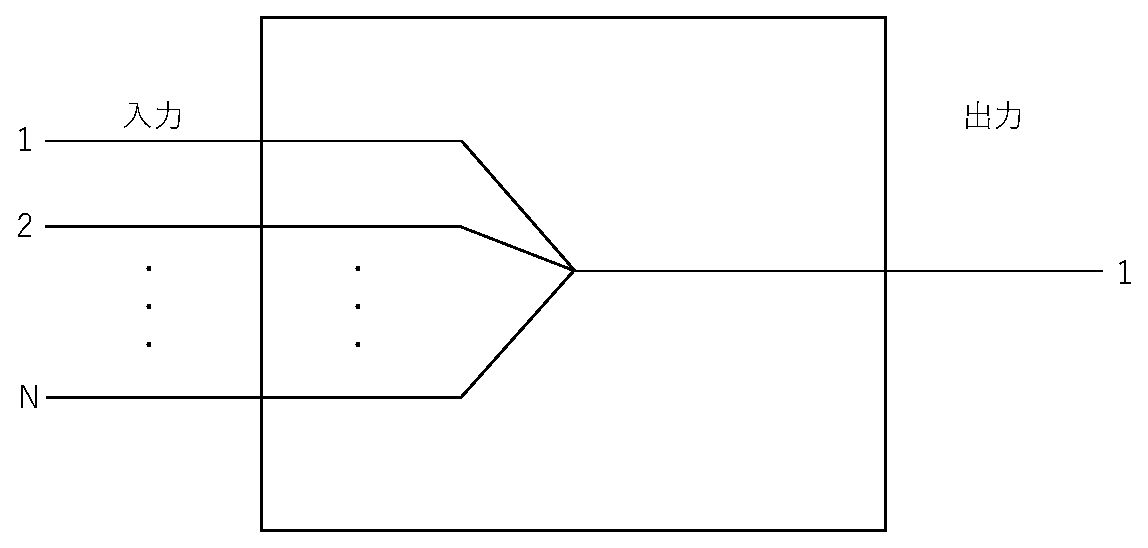
\includegraphics[keepaspectratio, scale=0.4]{fig/3/lcoup3.eps}
\label{fig:lcoup3}
}
\subfigure[光スターカプラ:N入力N出力]{
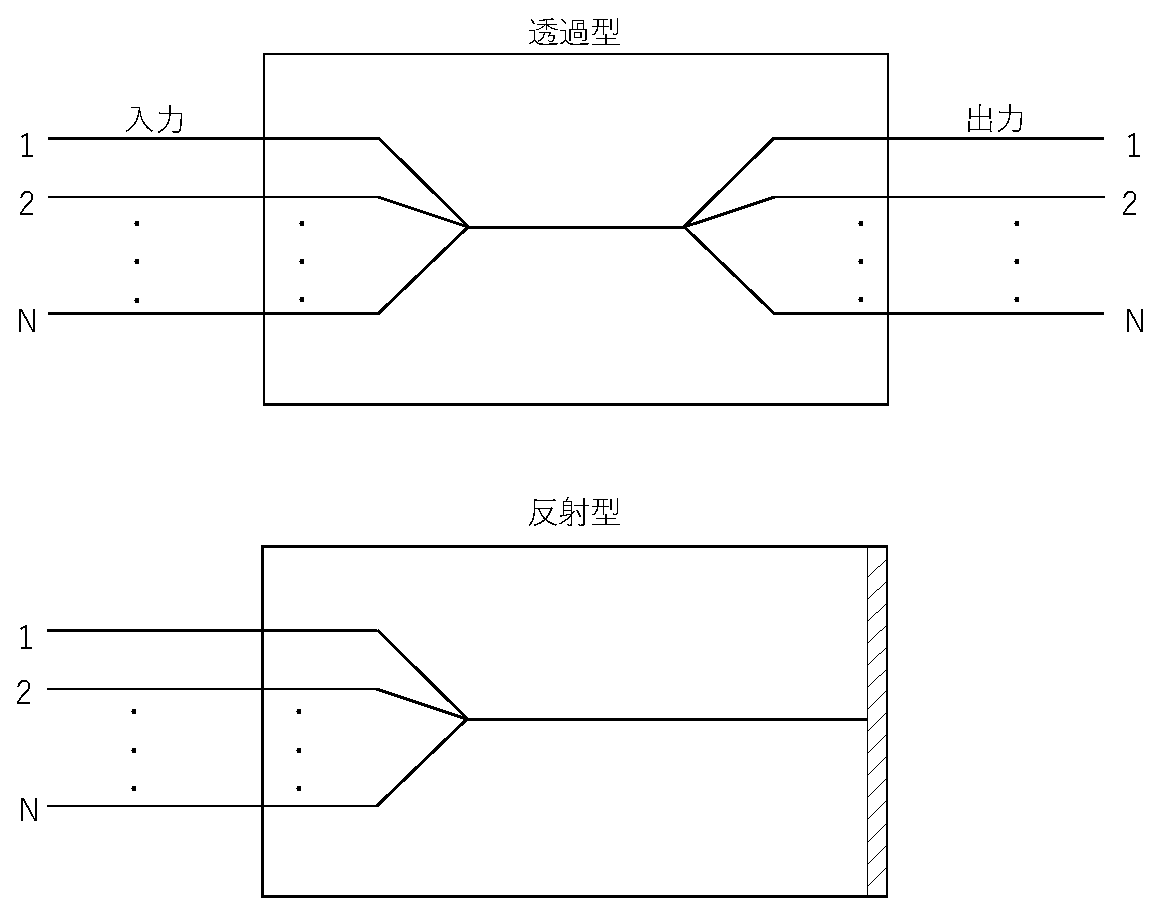
\includegraphics[keepaspectratio, scale=0.4]{fig/3/lcoup4.eps}
\label{fig:lcoup4}
}
\caption{光カプラの分類}
\label{fig:lcoup}
\end{center}
\end{figure}

\subsubsection{光遅延素子}
光遅延素子は光伝搬信号に伝搬遅延を付加できる素子のことを指す.
その実現は様々な方法があり,いずれの方法を用いても遅延を付加する際には損失が発生する.

\subsection{ナノフォトニクスの性質}
ナノフォトニクスとは,ナノ加工技術をベースとして,近接場光の性質を活かした技術である.
近接場光とは物質の表面付近に局在する非伝播な電磁場であり,その局在範囲は光の波長と同程度かそれに比べ小さい.
近接場光の概要を図\ref{fig:kinsetu}に示す.
物質から遠ざかるにつれて電磁場は減少するため,その特徴からエバネッセント光とも呼ばれる.
屈折率が大きい媒質から屈折率の小さい媒質に光を入射させる.
この場合ある角度を超えると,光は境界面を通過せず全て反射する.
この現象を全反射と言う.物質表面に全反射が起こるように光を入射した際,反射が起こっている物質境界面付近では局在する電磁場が発生する.
この電磁場光がエバネッセント光である.
エバネッセント光が発生した際,境界面から離れる方向に電磁場が弱くなる.
図\ref{fig:eva2}はエバネッセント光が発生する様子である.
\begin{figure}[t!]
\begin{center}
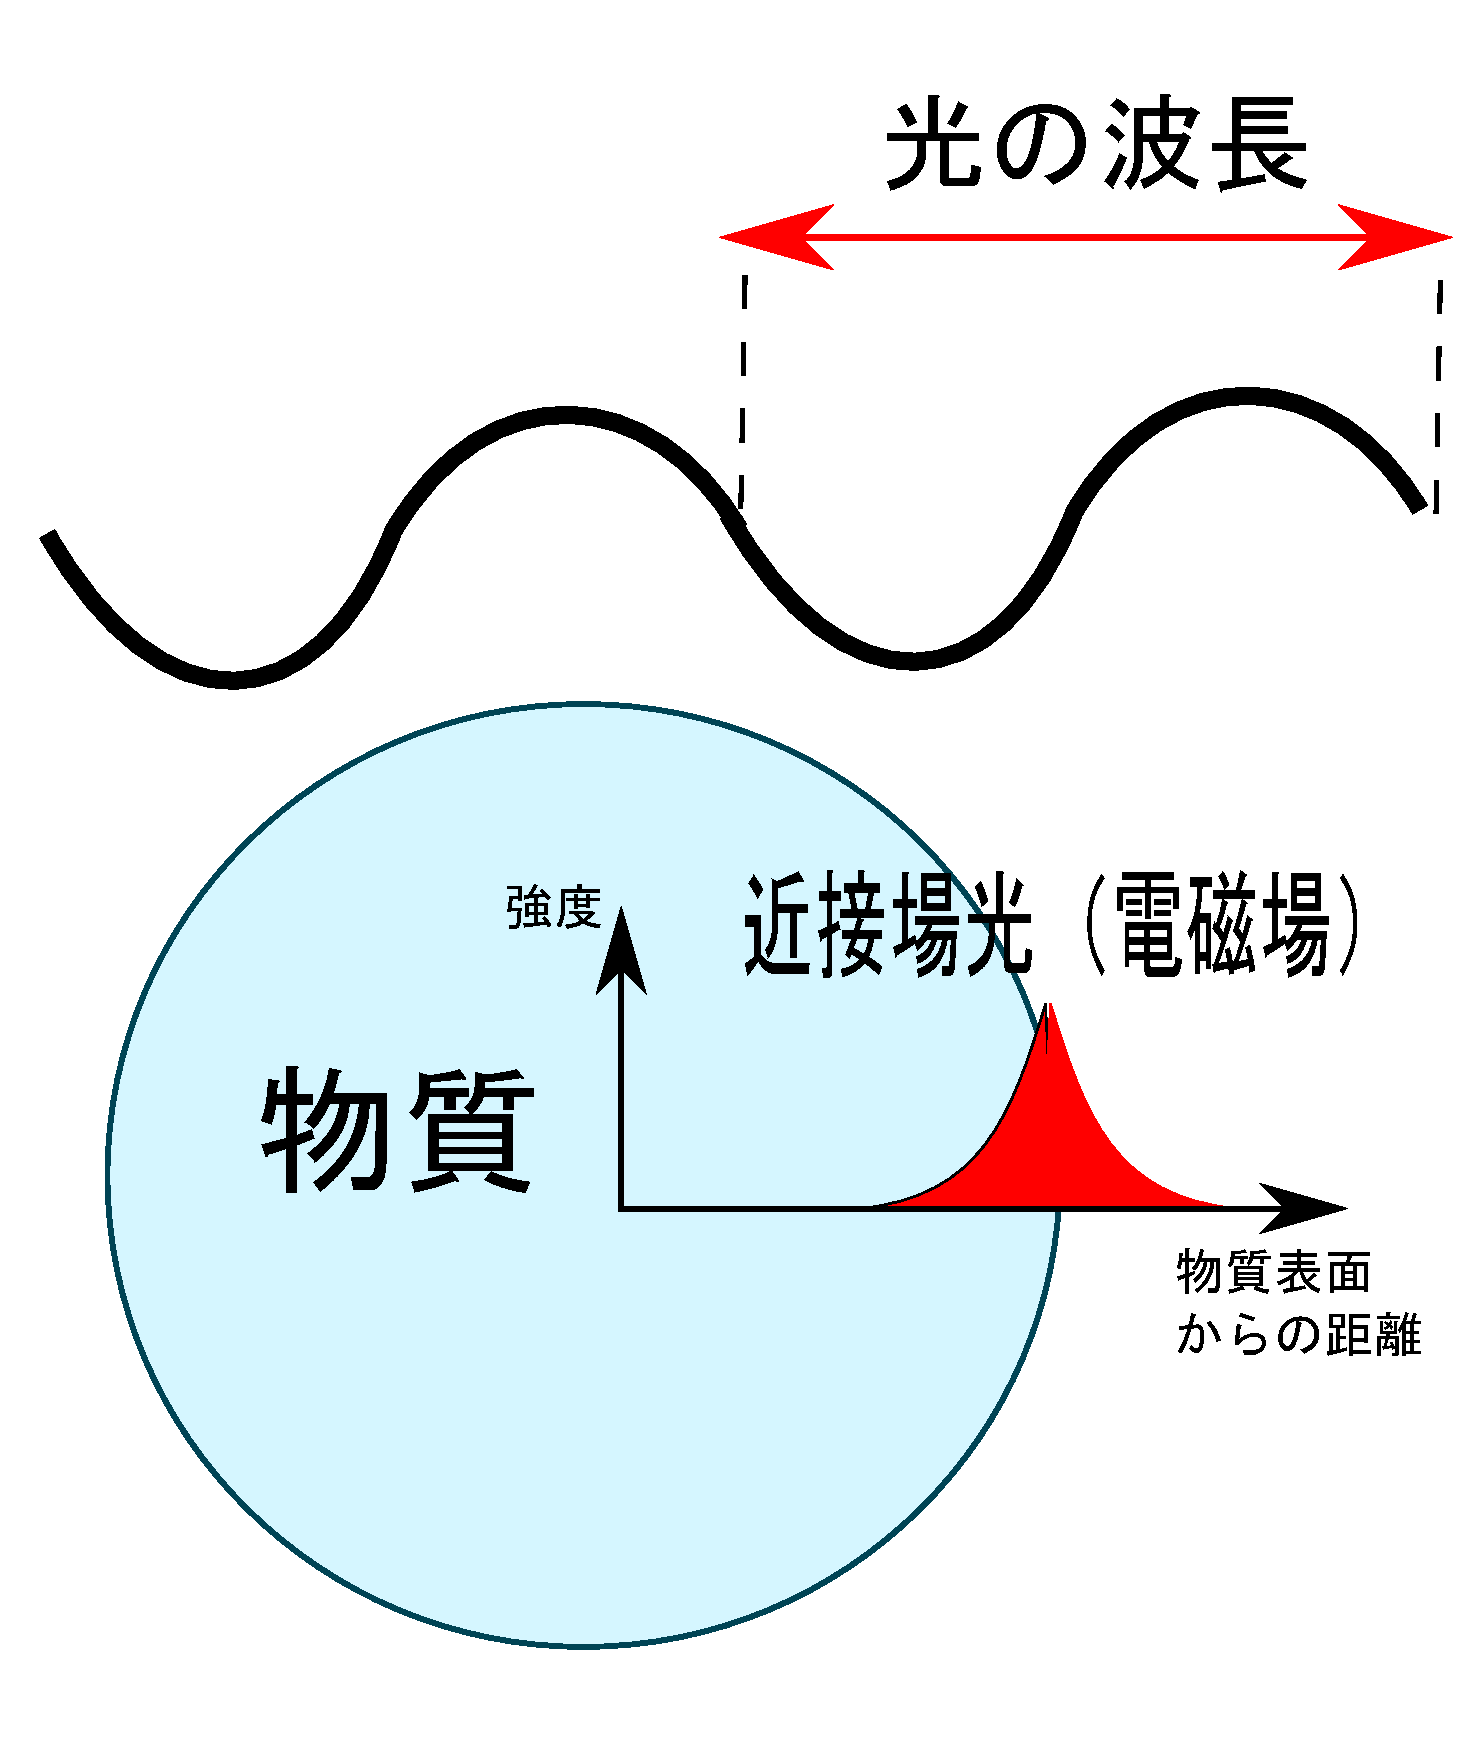
\includegraphics[keepaspectratio,scale=0.3]{fig/3/kinsetu.pdf}
\caption{近接場光}
\label{fig:kinsetu}
\end{center}
\end{figure}
\begin{figure}[t!]
\begin{center}
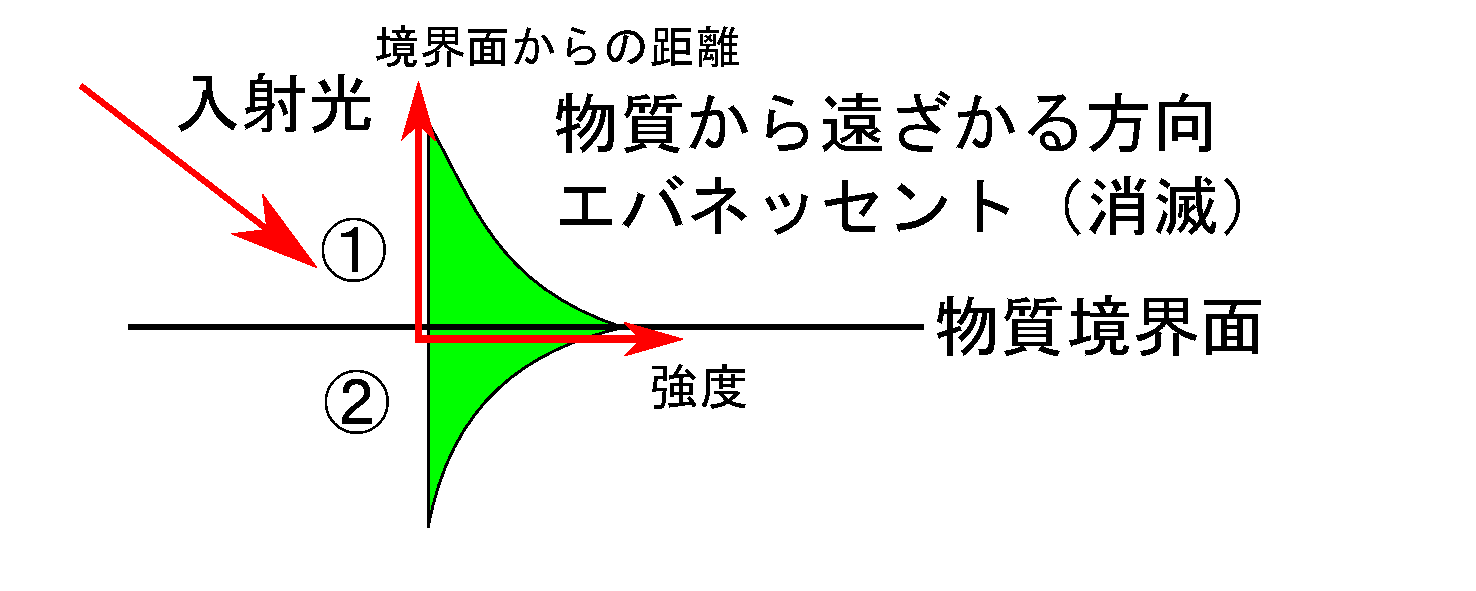
\includegraphics[keepaspectratio,scale=0.4]{fig/3/evanesent2.pdf}
\caption{エバネッセント光}
\label{fig:eva2}
\end{center}
\end{figure}
従来の光通信で広く使われている光素子の素材はガラスである.
これを半導体微細加工技術を用いて,半導体へと置き換える.
この技術によって半導体内を光が伝送できる.
ガラスから半導体へと素材を変えただけでは,光素子のゲート長のスケールは$cmからmm$のサイズに小さくなる.
これを$ \mu m$のスケールにするためには,半導体などのナノ加工技術がベースとしてある.
半導体のナノ加工技術が素子の加工技術のベースになり,近接場光の局在性をはじめとする近接場光にしかない特徴を活かして,
光信号をナノレベルで制御することが可能になって成り立つ技術がナノフォトニクスである.

\subsection{光デバイスとレースロジック}
前述した通り,光デバイスとは光伝搬信号を取り扱う素子を指す.
光伝搬信号の情報媒体は信号強度や位相,遅延時間といったアナログ量であり,
光伝搬信号はアナログ信号である.
電気デバイスであるCMOSトランジスタは電気信号を取り扱い,
その電気信号はデジタル信号である.
扱う信号がデジタル信号であるかアナログ信号であるかは二つのデバイスの大きな違いである.

また,レースロジックは動的計画法で解くことができる最適化問題の答えを
遅延時間というアナログ量で表現するアプローチである.

本研究では,情報媒体にアナログ量を取り扱う光デバイスと
レースロジックとの親和性に着目した.
ナノフォトニクック・デバイスをはじめとする
光デバイスの光速での信号処理という特徴から,
CMOSデバイスを用いたレースロジック回路よりも性能において優位になると考え,
ナノフォトニック・デバイスを用いたレースロジック回路を提案する.

\section{提案回路}
ナノフォトニック・デバイスを用いたレースロジック回路も,
図\ref{fig:ctrl}に示すようにコントロールと光伝搬出力信号のアレイ伝搬遅延時間を
計測する部分とアレイからなるものを想定する.
本論文では,光レースロジックアレイのセル構造を提案する.
図\ref{fig:lightracelogiccell}に光レースロジックアレイのセルの概要を示す.
\begin{figure}[t!]
\begin{center}
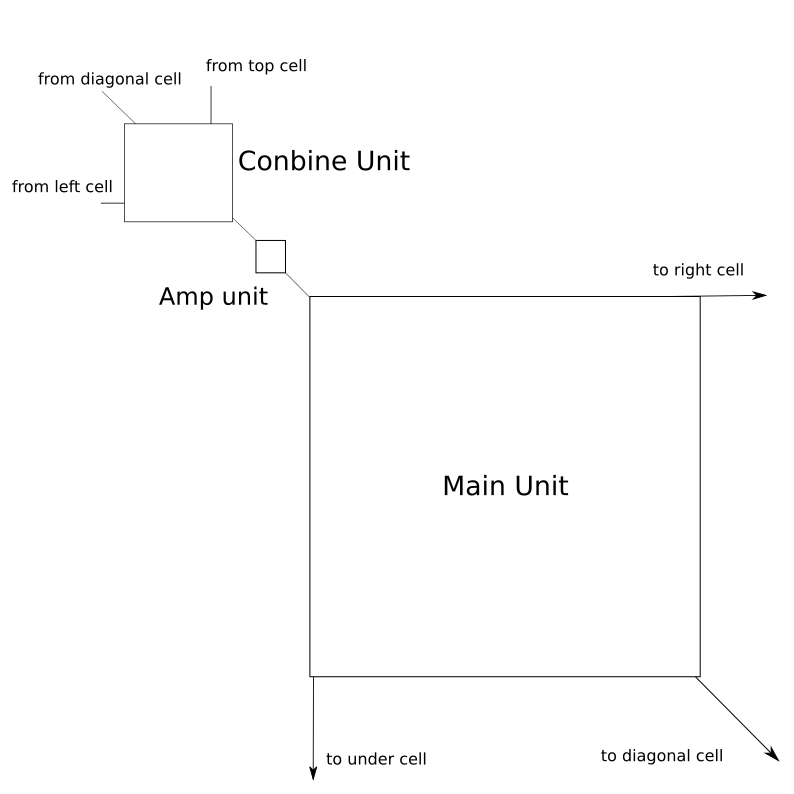
\includegraphics[keepaspectratio,scale=0.5]{fig/3/lightracelogic_cell_1.png}
\caption{光Race logic回路におけるセルの概要}
\label{fig:lightracelogiccell}
\end{center}
\end{figure}

セルは3つのユニットから構成される.
合波ユニットは,左,斜上,上のセルからの光伝搬入力信号を合波させるユニットである.
最長経路探索や最短経路探索,回路に設定する競争条件に合わせてその処理・構成が変わる.
その後,光伝搬信号はアンプユニットで光強度を増幅された後,メインユニット到達する.
メインユニットでは光伝搬信号の分波と任意の処理を施して,
光伝搬信号を次のセルへと出力する.
このユニットの構成と処理は回路に設定された競争条件によって変化する.
また,同期・非同期の処理に関しては合波ユニットもしくはメインユニット,あるいはその両方の構成で設定する.
対象とするアプリケーションや設定する競争条件によって,セルの構成は詳細に決定する.

本論文ではDNAのグローバル配列アラインメントスコア計算を対象とした
非同期型光レースロジック回路のアレイを提案する.
今回の提案回路で非同期型の構成を選択したのは,
光伝搬信号は蓄積が困難であるという点を考慮した結果である.
計算に用いるスコアマトリクスは式\ref{eq:mchun}を用いて求めた.
そのスコアマトリクスを図\ref{fig:scorematrix_3}に示す.
最下行と最右列はギャップスコアを表している.
\begin{figure}[t!]
\begin{center}
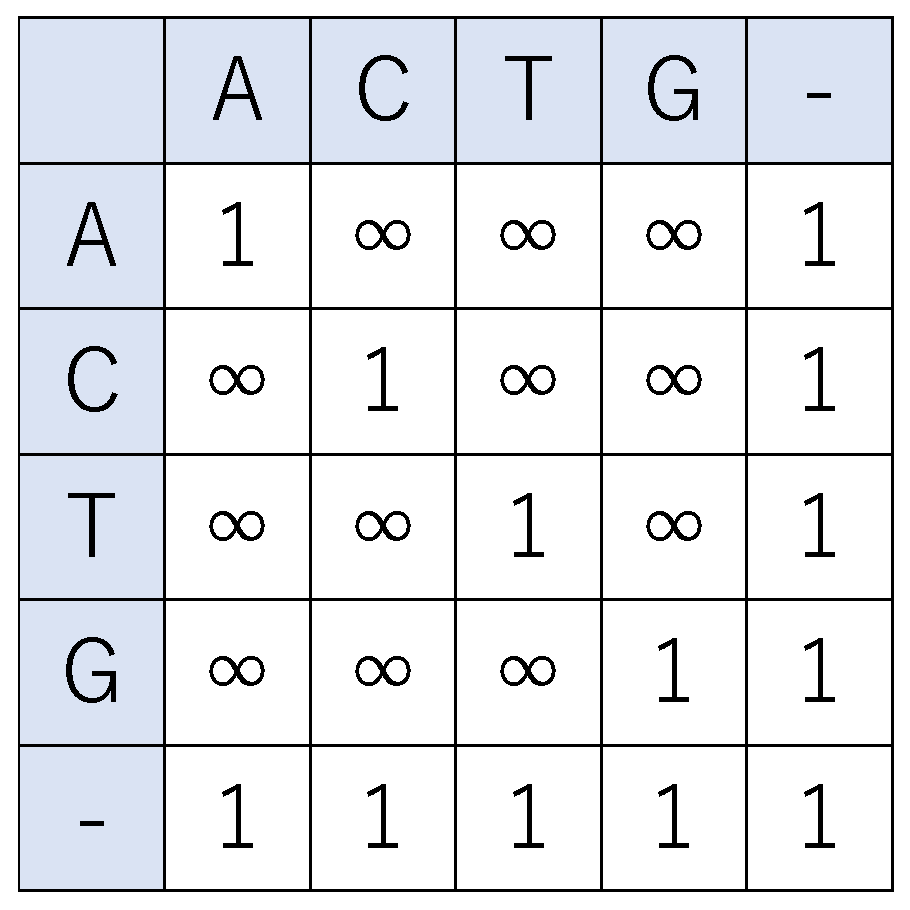
\includegraphics[keepaspectratio,scale=0.4]{fig/3/scorematrix.eps}
\caption{使用するスコアマトリクス}
\label{fig:scorematrix_3}
\end{center}
\end{figure}

図\ref{fig:proposalcell}に提案する回路のセル構造を示す.
\begin{figure}[t!]
\begin{center}
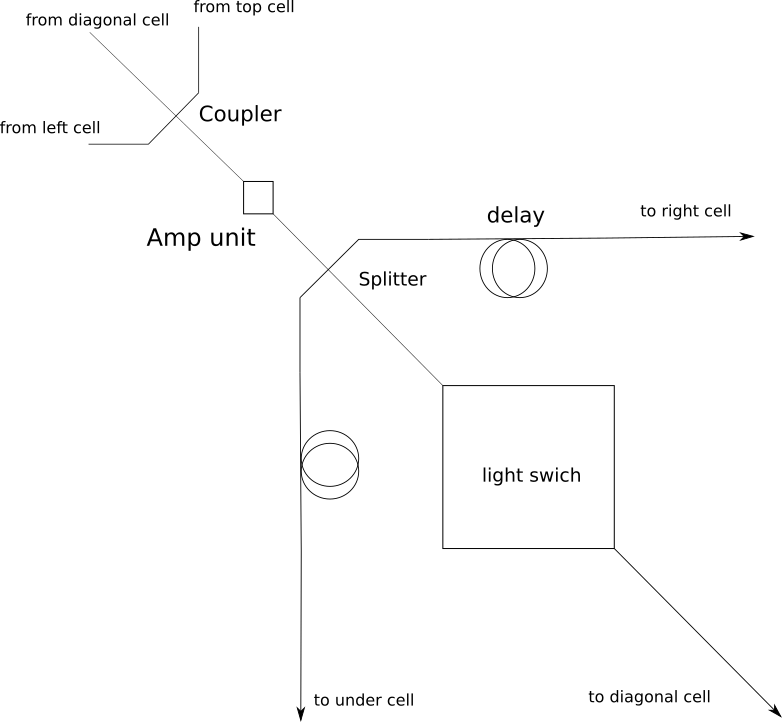
\includegraphics[keepaspectratio,scale=0.5]{fig/3/lightracelogic_cell_6.png}
\caption{提案回路のセル構造}
\label{fig:proposalcell}
\end{center}
\end{figure}


提案回路のセルにおける,3つのユニットの構成・動作を述べる.
\begin{itemize}
\item 合波ユニット\\
\ \ このユニットでは3入力1出力の光カプラを用いて合波が行われる.
図\ref{fig:couplerunit}にその動作を示す.
\begin{figure}[t!]
\begin{center}
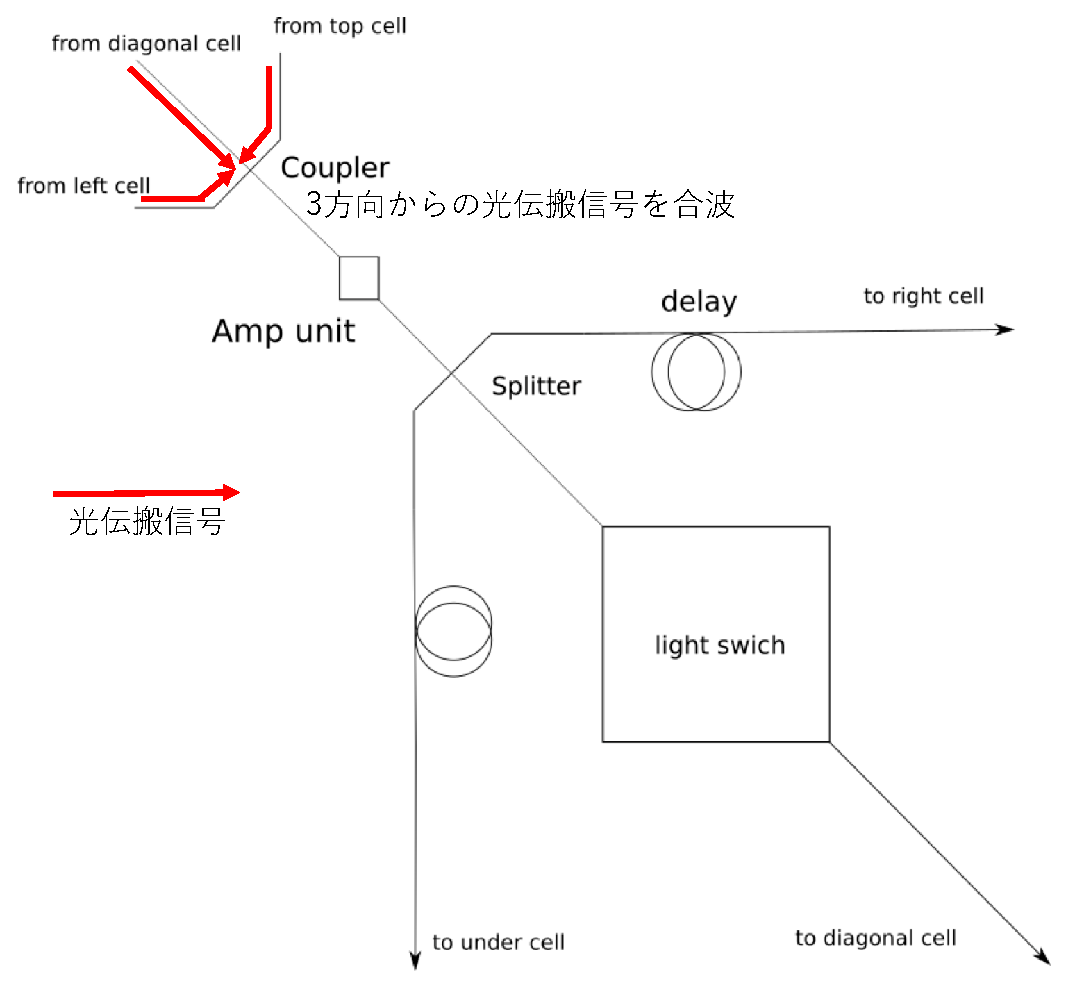
\includegraphics[keepaspectratio,scale=0.4]{fig/3/lightracelogic_cell_6_1.eps}
\caption{合波ユニットの挙動}
\label{fig:couplerunit}
\end{center}
\end{figure}
この時,3方向それぞれからの光入力信号が光カプラに到達するまでの時間は
同じでなければならない.
\item アンプユニット\\
\ \ 合波ユニットを経た光伝搬信号は,光アンプにて増幅される.
図\ref{fig:ampunit}にその動作を示す.
\begin{figure}[t!]
\begin{center}
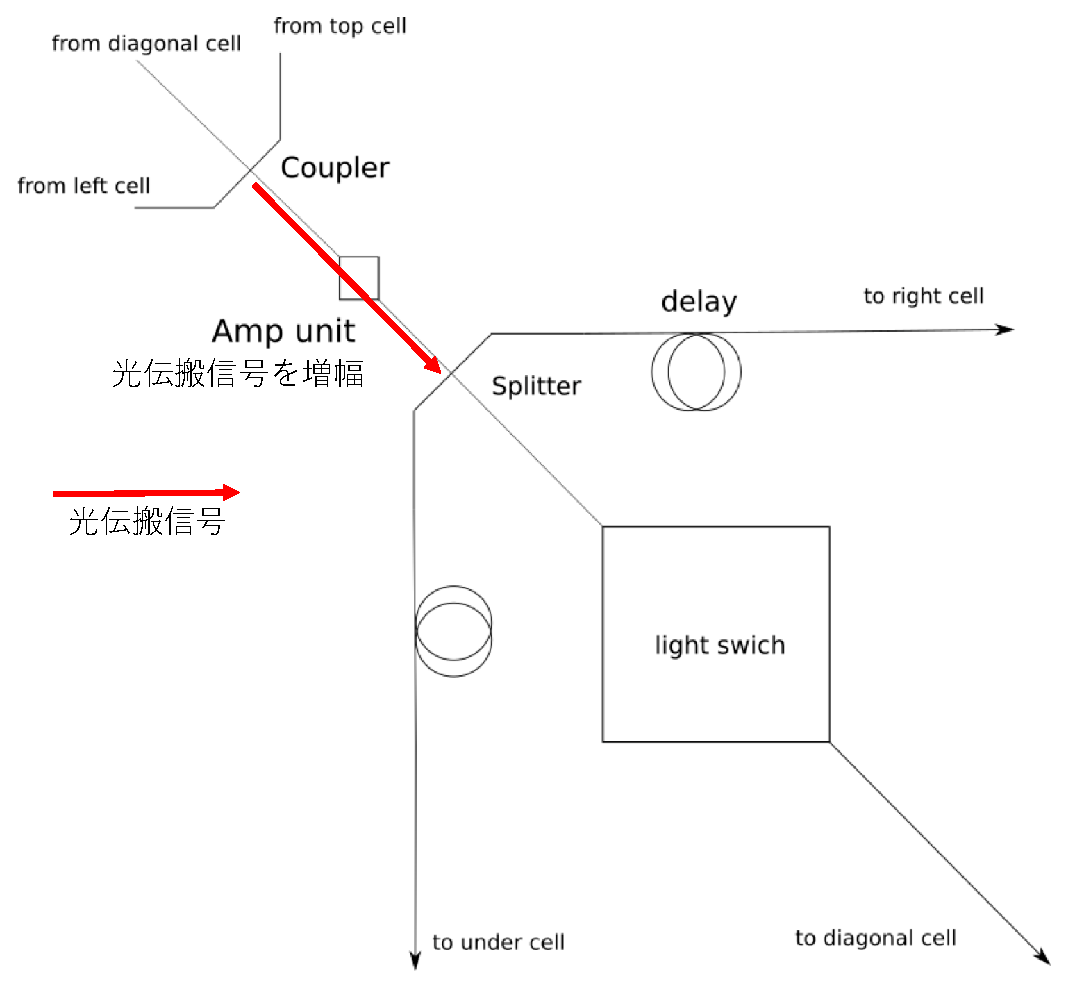
\includegraphics[keepaspectratio,scale=0.4]{fig/3/lightracelogic_cell_6_2.eps}
\caption{アンプユニットの挙動}
\label{fig:ampunit}
\end{center}
\end{figure}
この光アンプでは,光伝搬信号が各素子を伝搬した際の強度損失を
補う役割をしている.
\item メインユニット\\
\ \ メインユニットに求められる機能は右,下,斜下の3つの経路への分波と,
各伝搬経路ごとにスコアマトリクスに基づく重み付けである.
右,下,斜下の3つの経路への分波は,図\ref{fig:mainunit_s}に挙動を示すように
1入力3出力の光カプラを用いて行われる.\\
\begin{figure}[t!]
\begin{center}
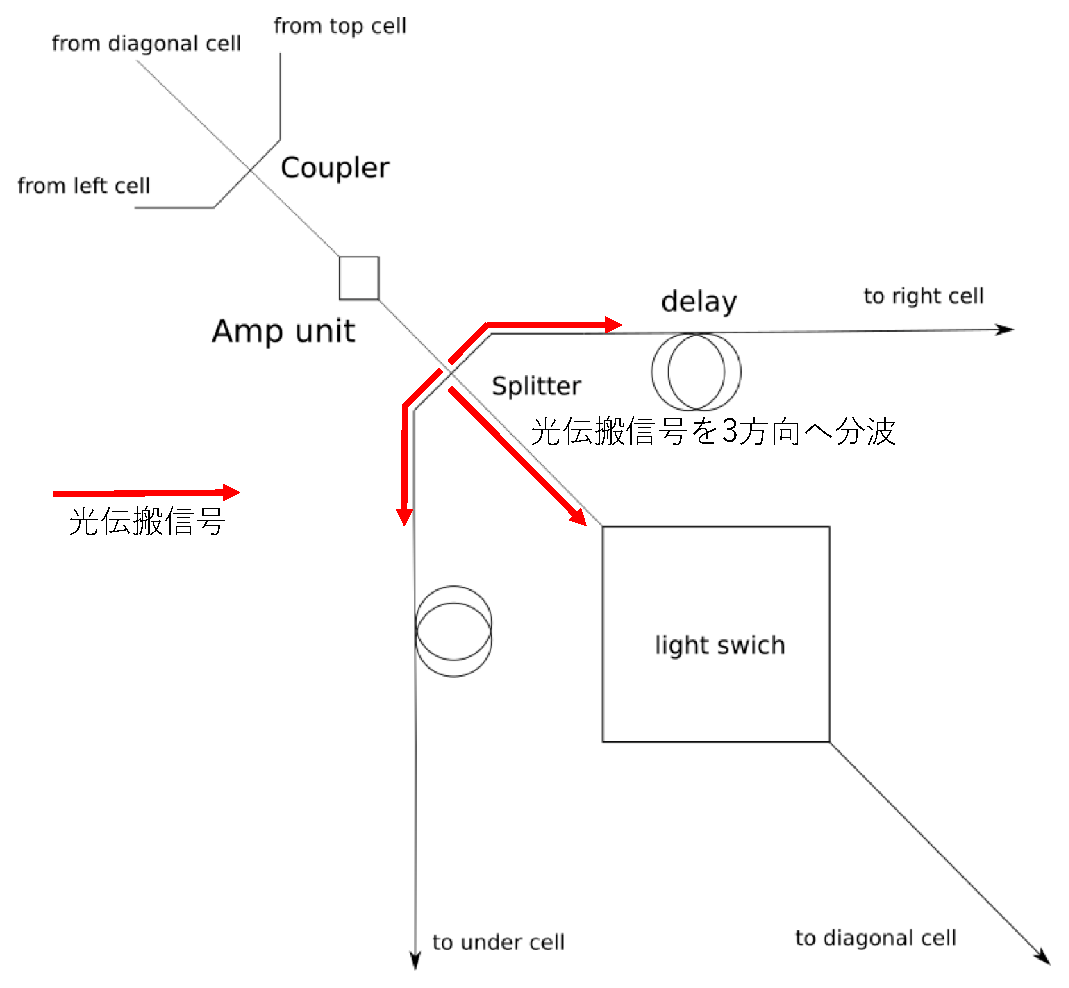
\includegraphics[keepaspectratio,scale=0.4]{fig/3/lightracelogic_cell_6_3.eps}
\caption{メインユニット・1入力3出力光カプラの挙動}
\label{fig:mainunit_s}
\end{center}
\end{figure}
\ \ 次に各伝搬経路ごとのスコアマトリクスに基づいての重み付けについて説明する.
斜下への伝搬経路では,文字列の一致・不一致によってそれぞれ違う重み付けがされなければならない.
今回使用するスコアマトリクスにおいて,一致スコアは1,不一致スコアは$\infty$である.
このスコアに基づく重み付けを行うため,光スイッチを使用した.
光スイッチのオン/オフを決定する制御信号は,コントロール部分において
比較する文字列が一致した場合オン動作となるように,
不一致の場合にオフ動作となるように設定する.
光スイッチがオフ動作の時,光伝搬信号は斜下のセルに伝搬されない.
これは無限大の遅延時間を付加された,と考えることができ,
不一致スコアに対応した重み付けがされたとみなすことができる.
光スイッチがオン動作の時,光伝搬信号は光スイッチを通過し次のセルへと出力される.
この時の伝搬遅延時間をスコアマトリクスにおける一致スコアの1の重みを表す量として取り扱う.
右,下への伝搬経路はそれぞれ,文字列の欠損と挿入に対応し,
セルへの伝搬は文字列の一致・不一致に関わらず無条件に行われる.
文字列の欠損と挿入をギャップといい,ギャップに対応したスコアをギャップスコアという.
右,下への伝搬経路ではギャップスコアに基づく遅延が発生するように,
光遅延素子を設定する.
\ \ 今回使用するスコアマトリクスにおいては,ギャップスコアは1の重み付けをされており,
これは一致スコアと同じ重みである.
よって今回,光遅延素子で設定すべき遅延時間は,
光遅延素子を通過して次のセルへ出力されるまでの遅延時間が
斜め下への伝搬経路で発生する遅延時間と同じになるような量である.
3つの伝搬経路において遅延時間の重み付けをされた光伝搬信号は
次のセルへと伝搬される.\\
\ \ 図\ref{fig:mainunit}に比較する文字列が一致した場合と不一致の場合
それぞれのメインユニットの挙動を示す.
\begin{figure}[t!]
\begin{center}
\subfigure[比較する文字列が一致した場合のメインユニットの挙動]{
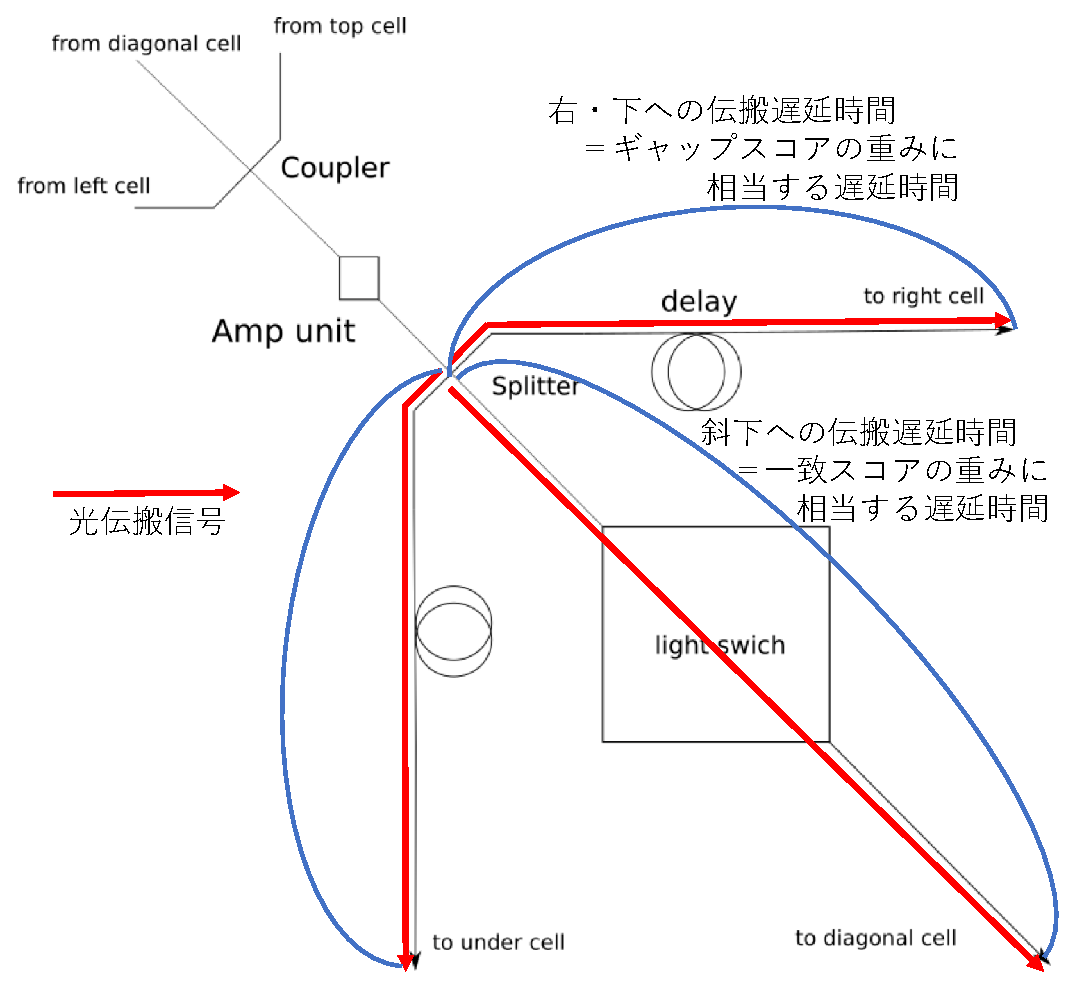
\includegraphics[keepaspectratio,scale=0.4]{fig/3/lightracelogic_cell_6_4.eps}}
\subfigure[比較する文字列が不一致の場合のメインユニットの挙動]{
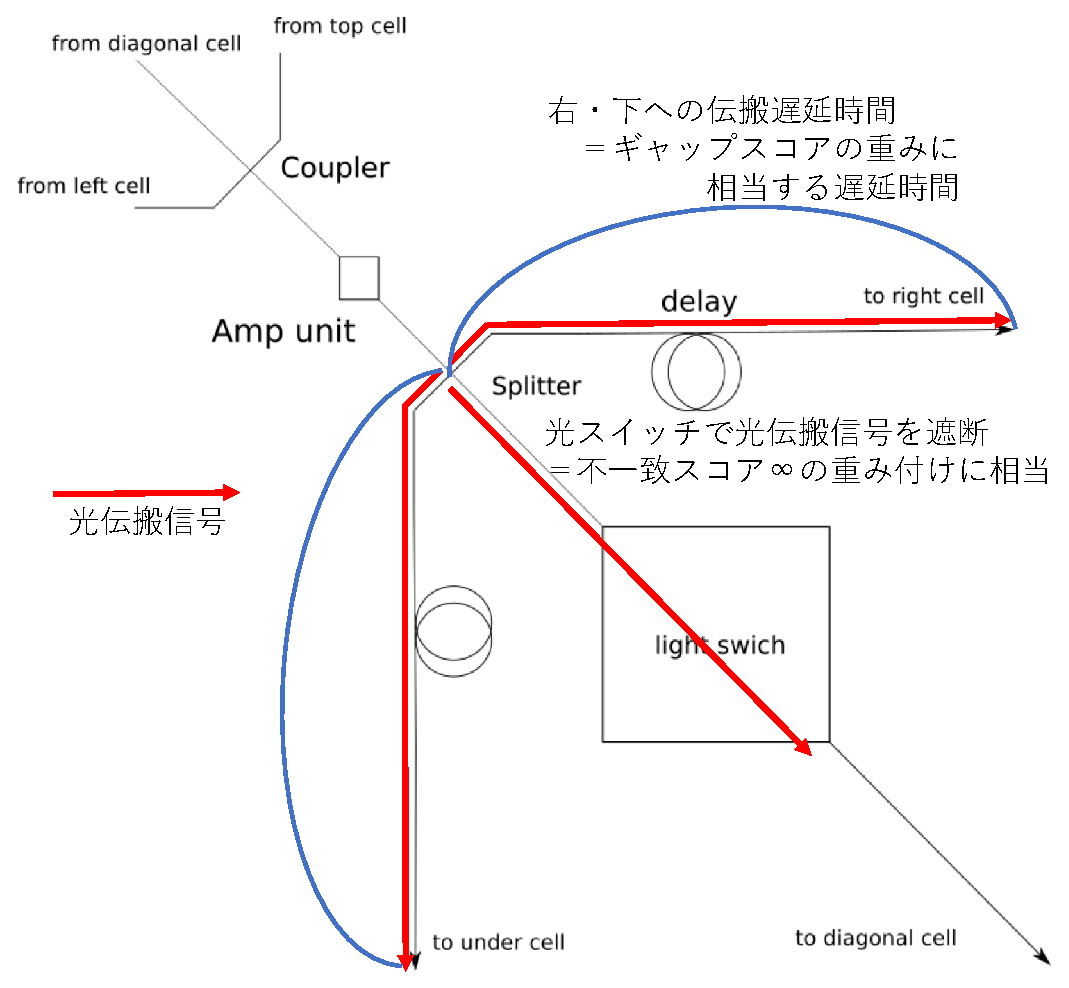
\includegraphics[keepaspectratio,scale=0.4]{fig/3/lightracelogic_cell_6_5.eps}}
\caption{メインユニットの挙動}
\label{fig:mainunit}
\end{center}
\end{figure}
\end{itemize}

このセルを並べることでDNA配列アラインメントスコア計算を対象とした
光レースロジックアレイを構築する.
配列長N=2の時の光レースロジックアレイの構成,
比較する文字列が完全に一致するの場合の光レースロジックアレイの挙動,
比較する文字列が完全に不一致の場合の光レースロジックアレイの挙動をそれぞれ
図\ref{fig:N=2},図\ref{fig:N=2_on},図\ref{fig:N=2_off}に示す.
\begin{figure}[t!]
\begin{center}
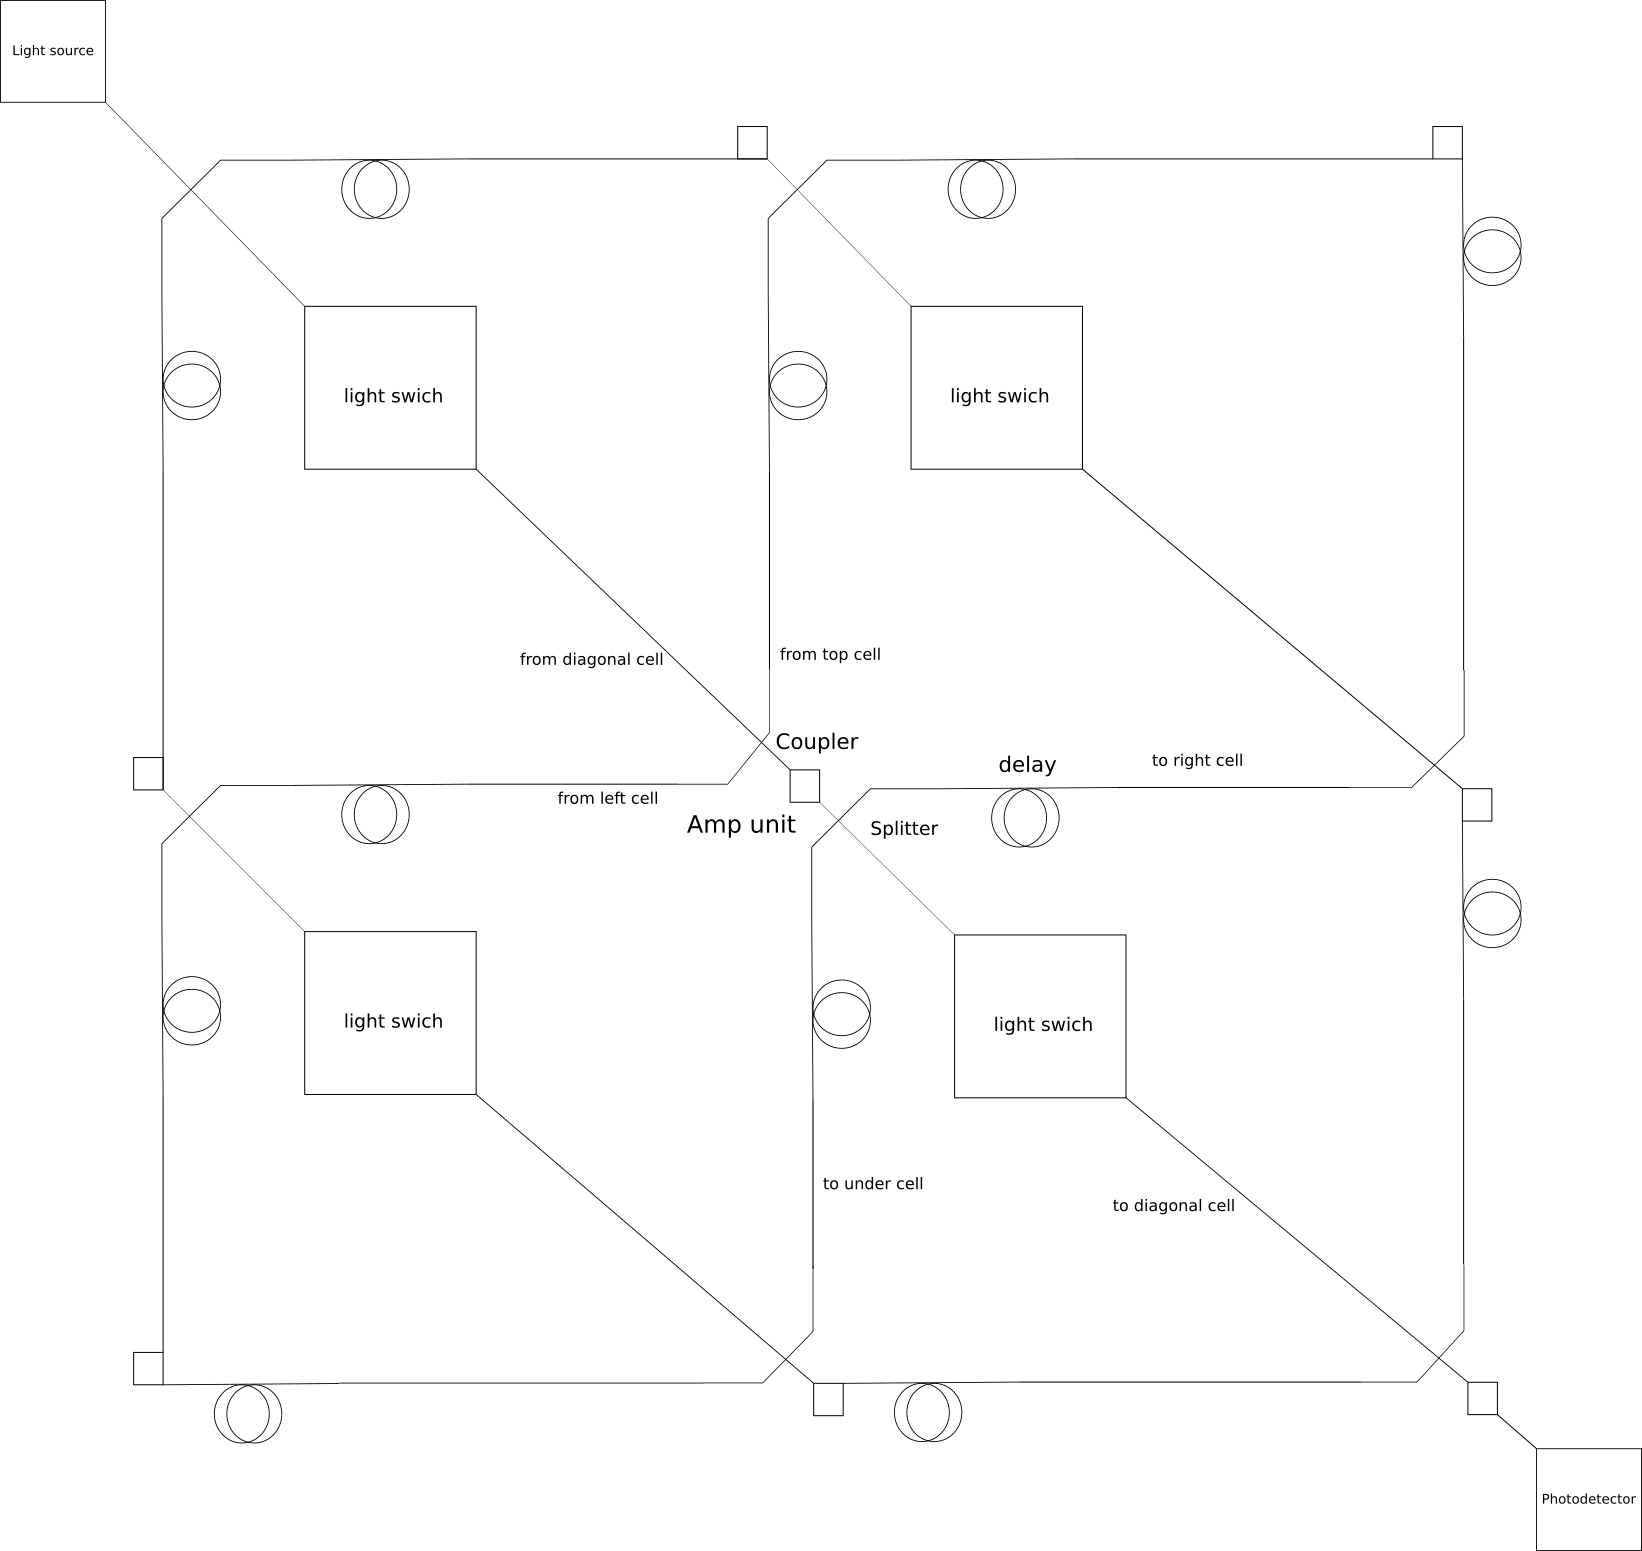
\includegraphics[keepaspectratio,scale=0.35]{fig/3/lightracelogic_N_2.png}
\caption{配列長N=2の光レースロジックアレイの構造}
\label{fig:N=2}
\end{center}
\end{figure}
図\ref{fig:N=2_on},図\ref{fig:N=2_off}の赤く示した経路が光伝搬信号が
伝搬している経路と到達する素子である.
\begin{figure}[t!]
\begin{center}
\subfigure[光伝搬信号入力から$1ns$後]{
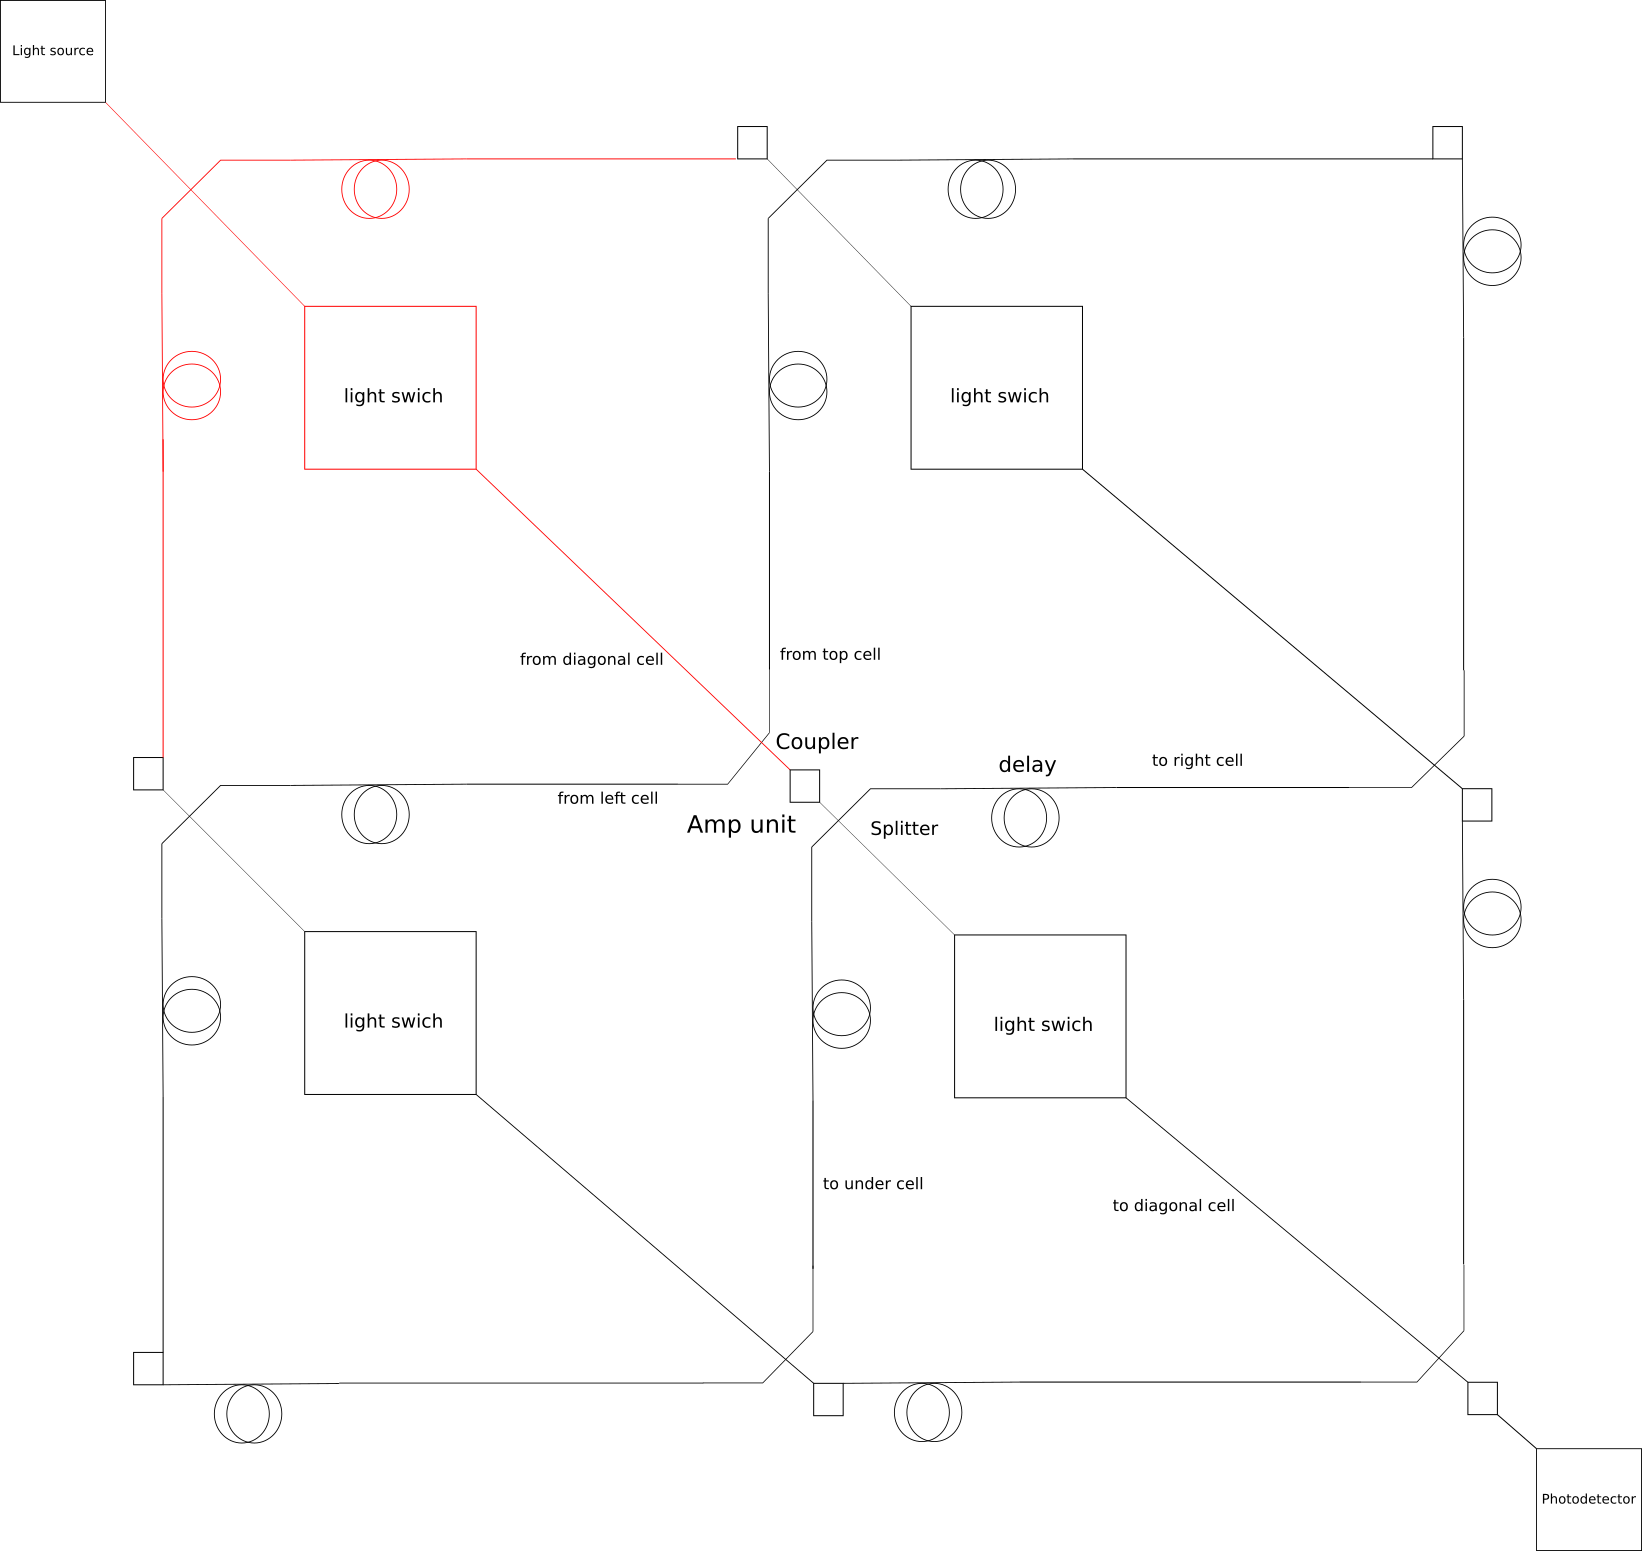
\includegraphics[keepaspectratio,scale=0.15]{fig/3/lightracelogic_N_2_on1.png}}
\subfigure[光伝搬信号入力から$2ns$後]{
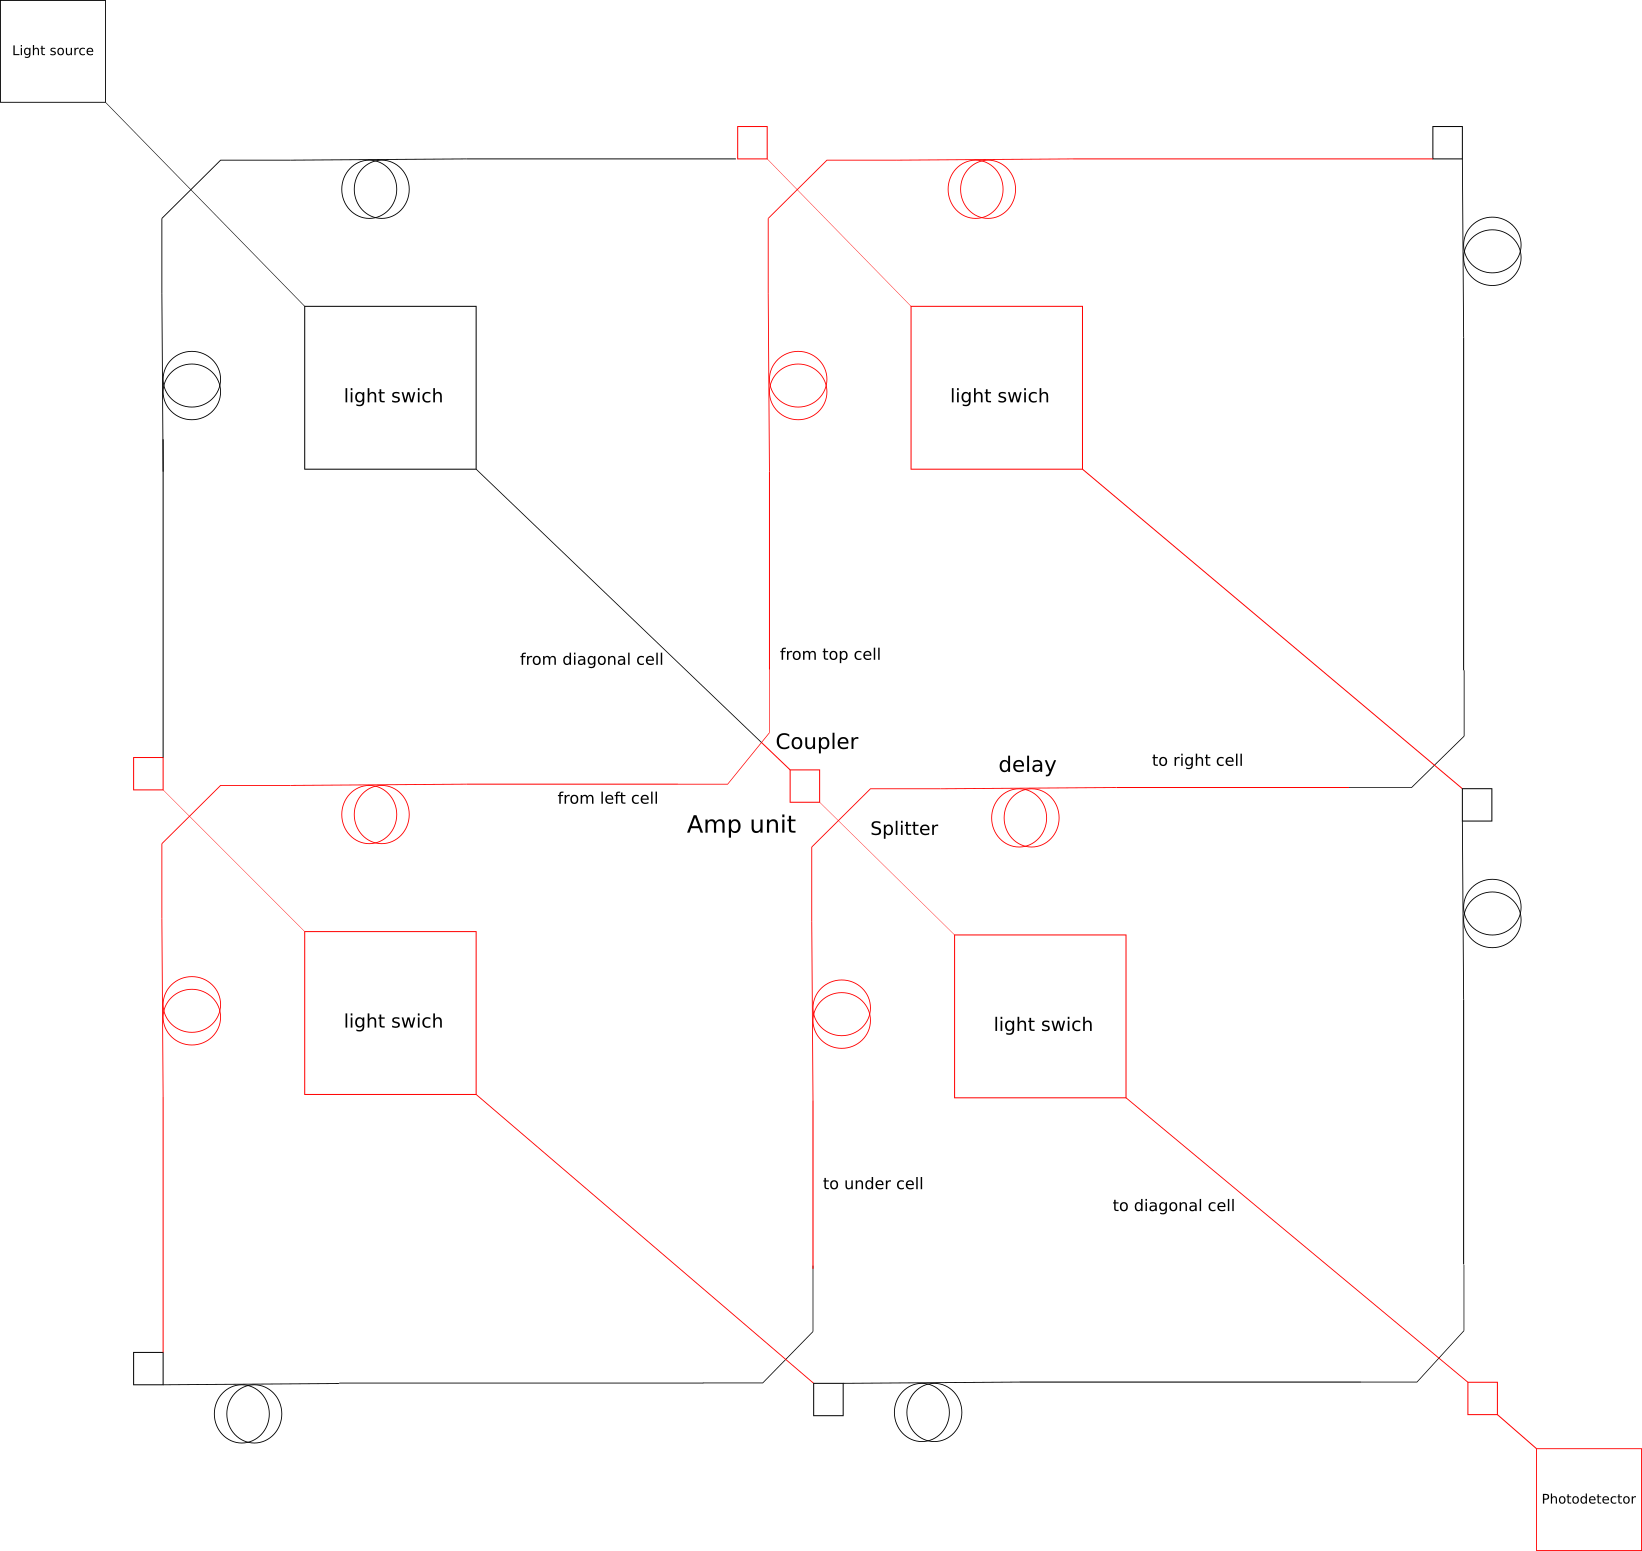
\includegraphics[keepaspectratio,scale=0.15]{fig/3/lightracelogic_N_2_on2.png}}\\
\subfigure[光伝搬信号入力から$3ns$後]{
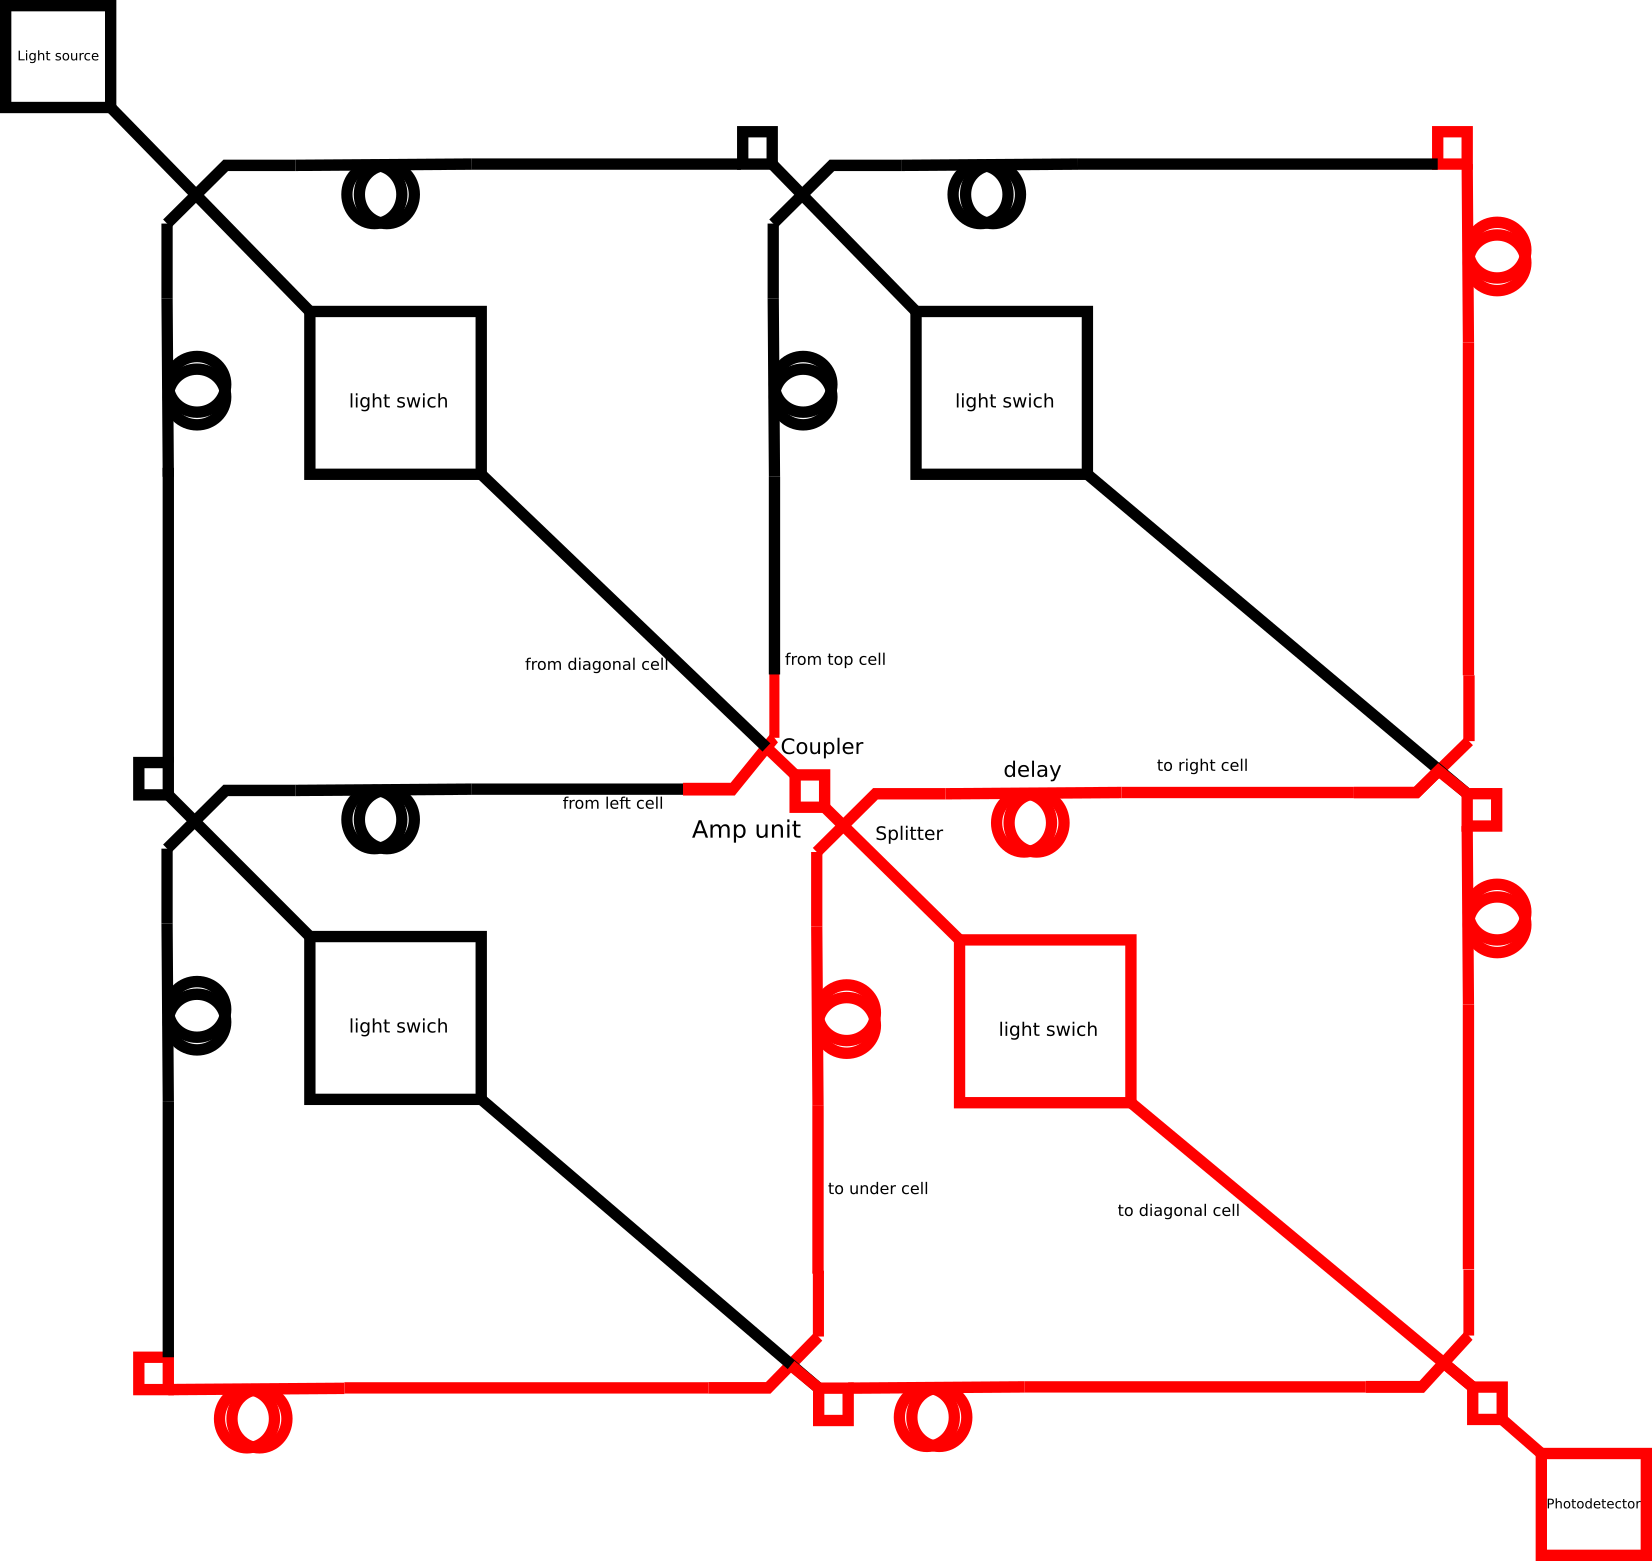
\includegraphics[keepaspectratio,scale=0.15]{fig/3/lightracelogic_N_2_on3.png}}
\subfigure[光伝搬信号入力から$4ns$後]{
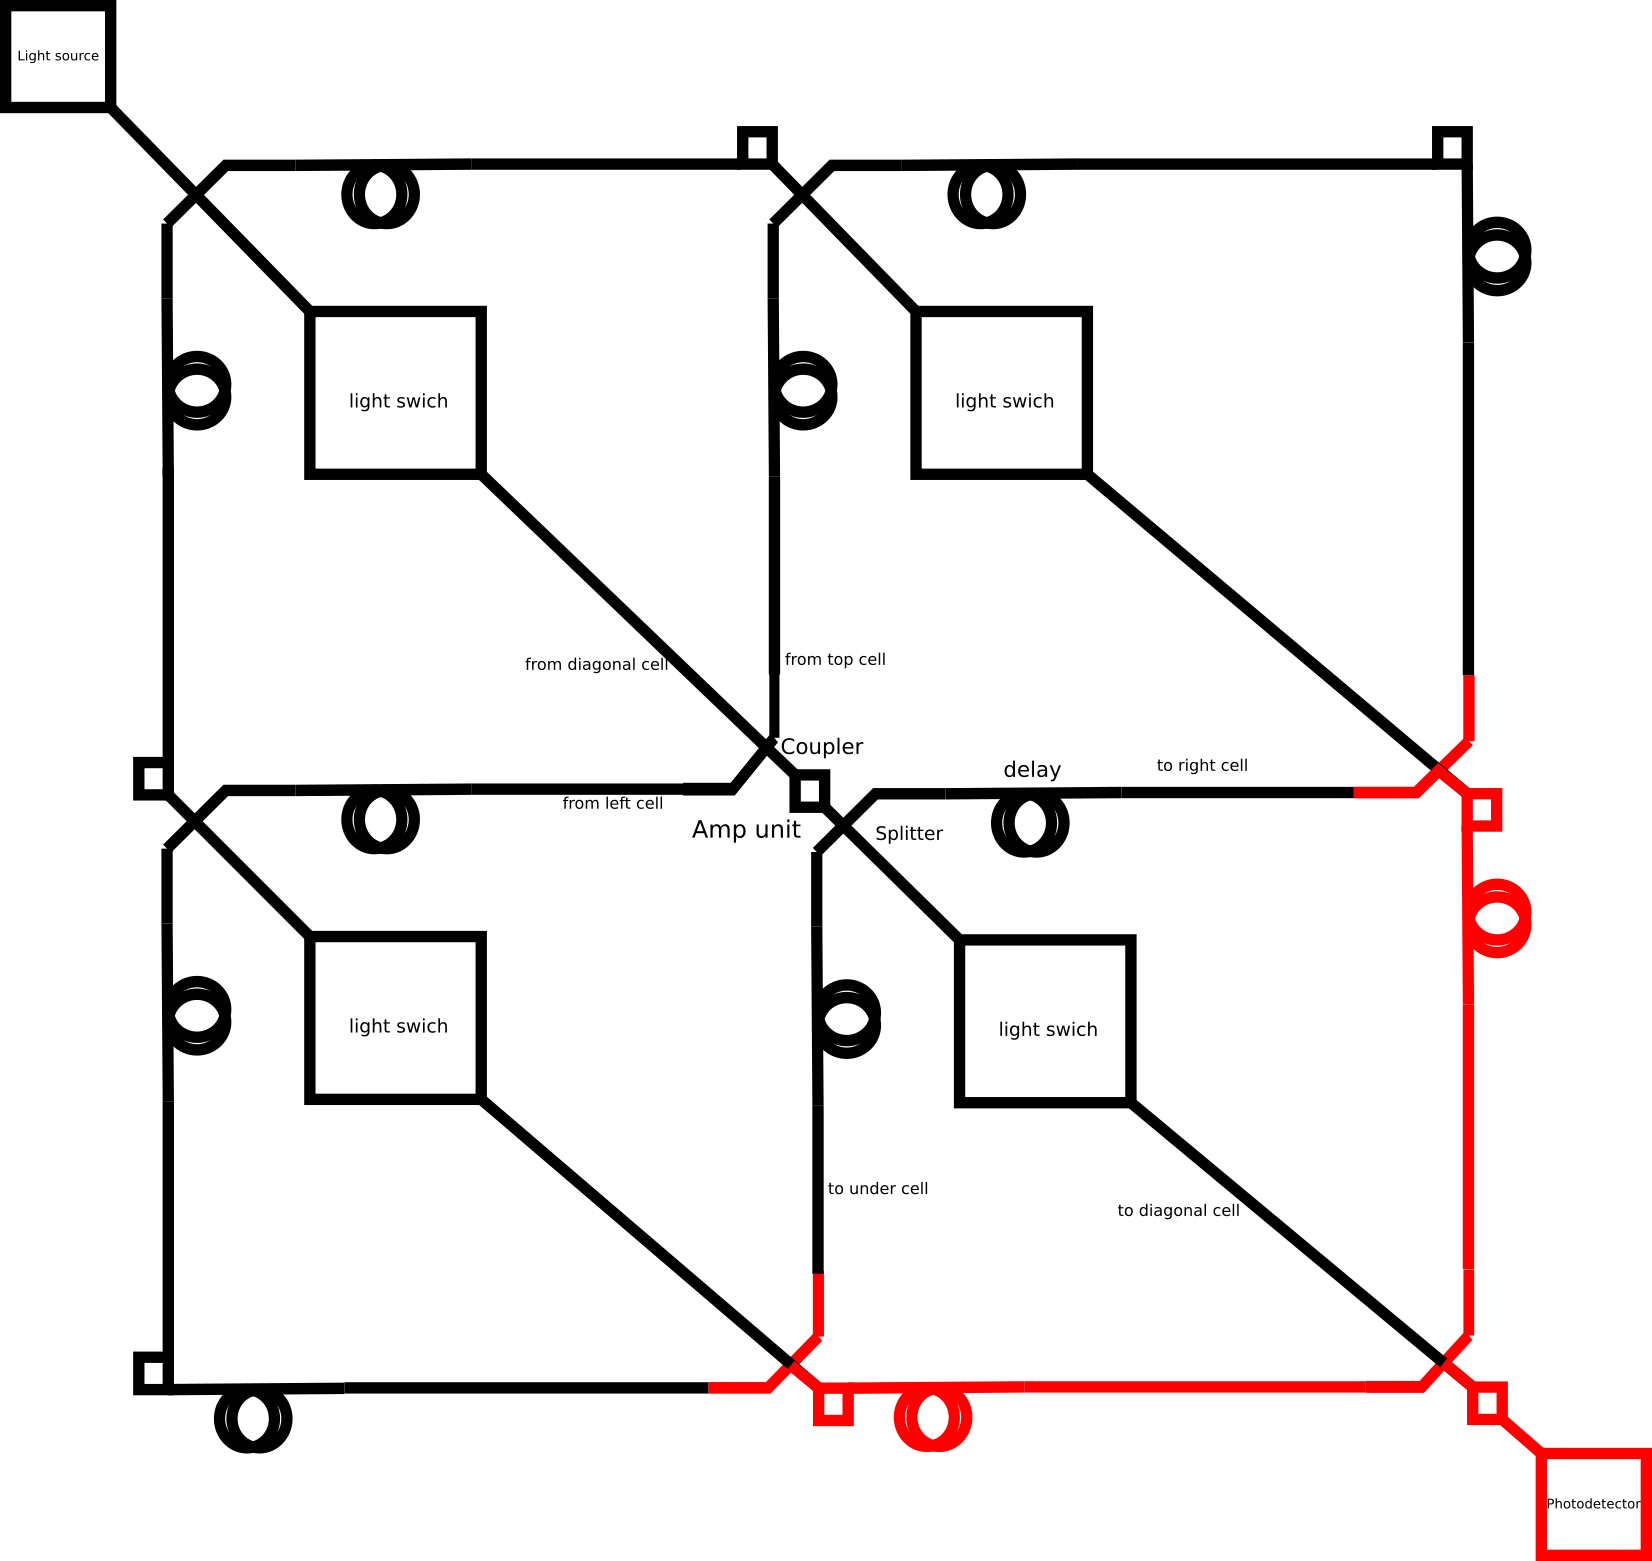
\includegraphics[keepaspectratio,scale=0.15]{fig/3/lightracelogic_N_2_on4.png}}\\
\caption{比較する文字列が完全に一致するの場合の光レースロジックアレイの挙動}
\label{fig:N=2_on}
\end{center}
\end{figure}
\begin{figure}[t!]
\begin{center}
\subfigure[光伝搬信号入力から$1ns$後]{
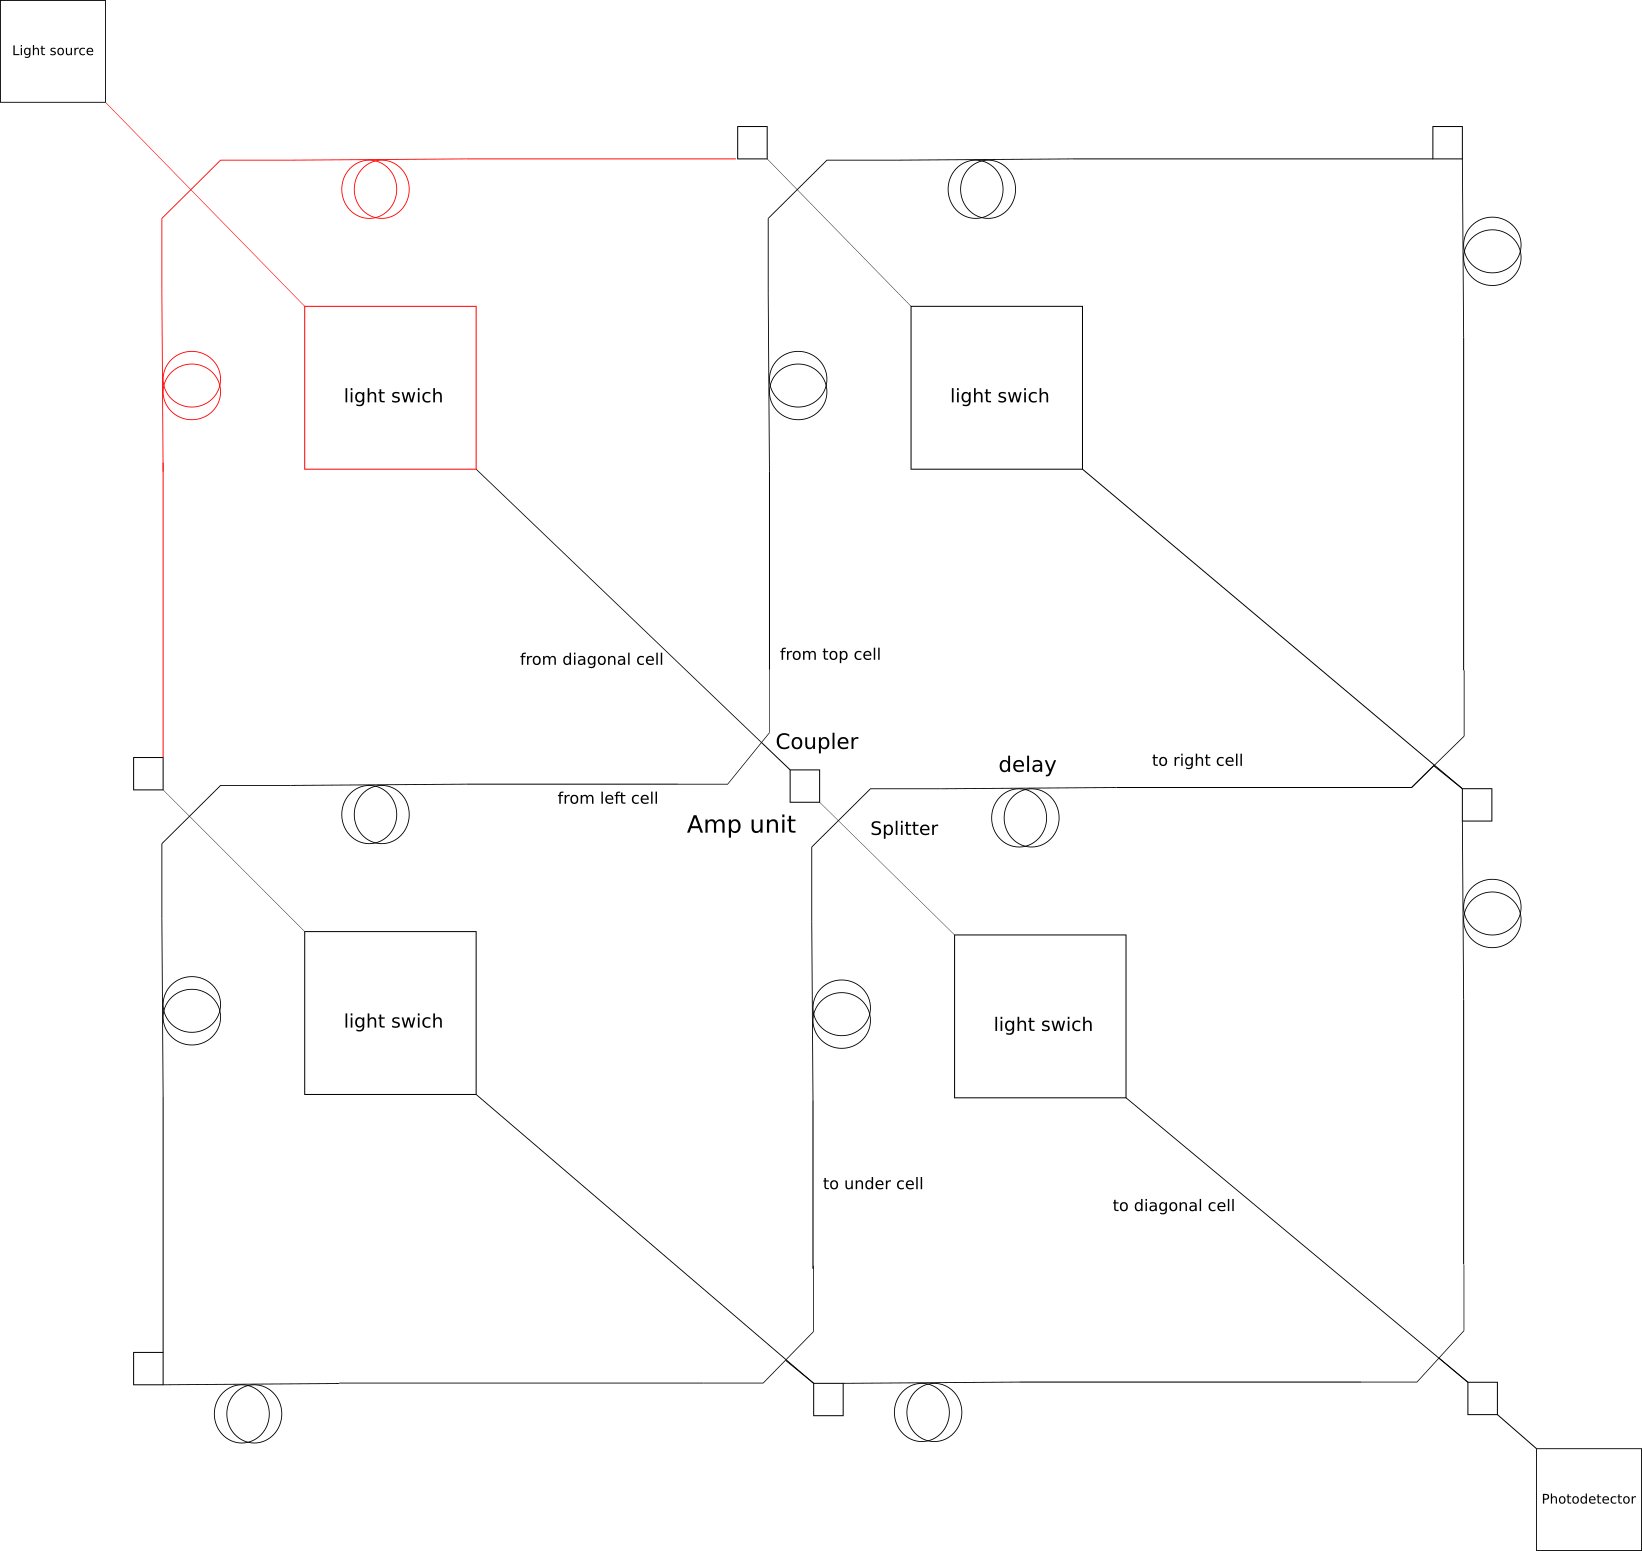
\includegraphics[keepaspectratio,scale=0.15]{fig/3/lightracelogic_N_2_off1.png}}
\subfigure[光伝搬信号入力から$2ns$後]{
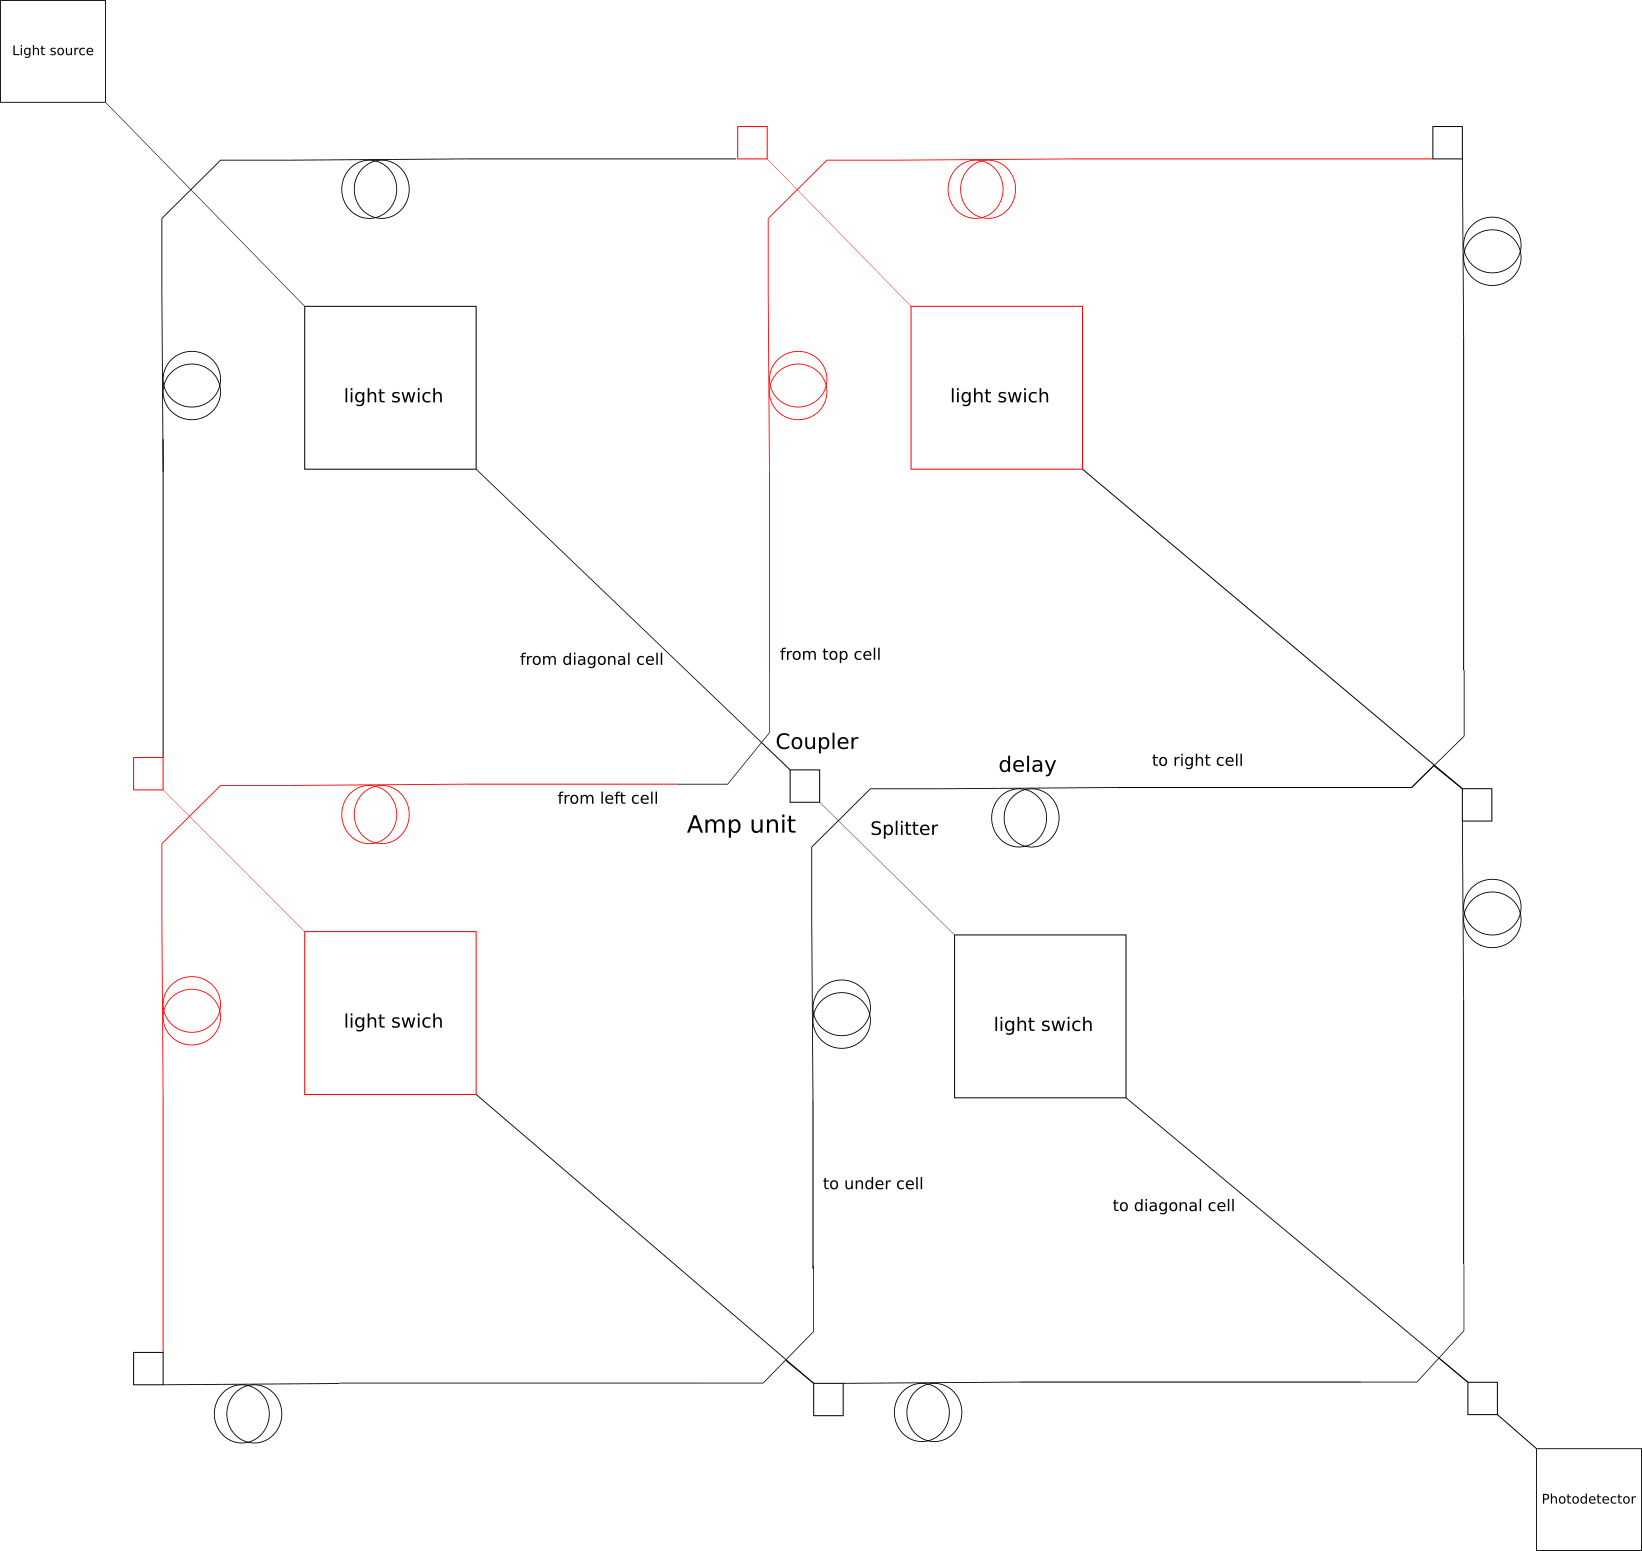
\includegraphics[keepaspectratio,scale=0.15]{fig/3/lightracelogic_N_2_off2.png}}\\
\subfigure[光伝搬信号入力から$3ns$後]{
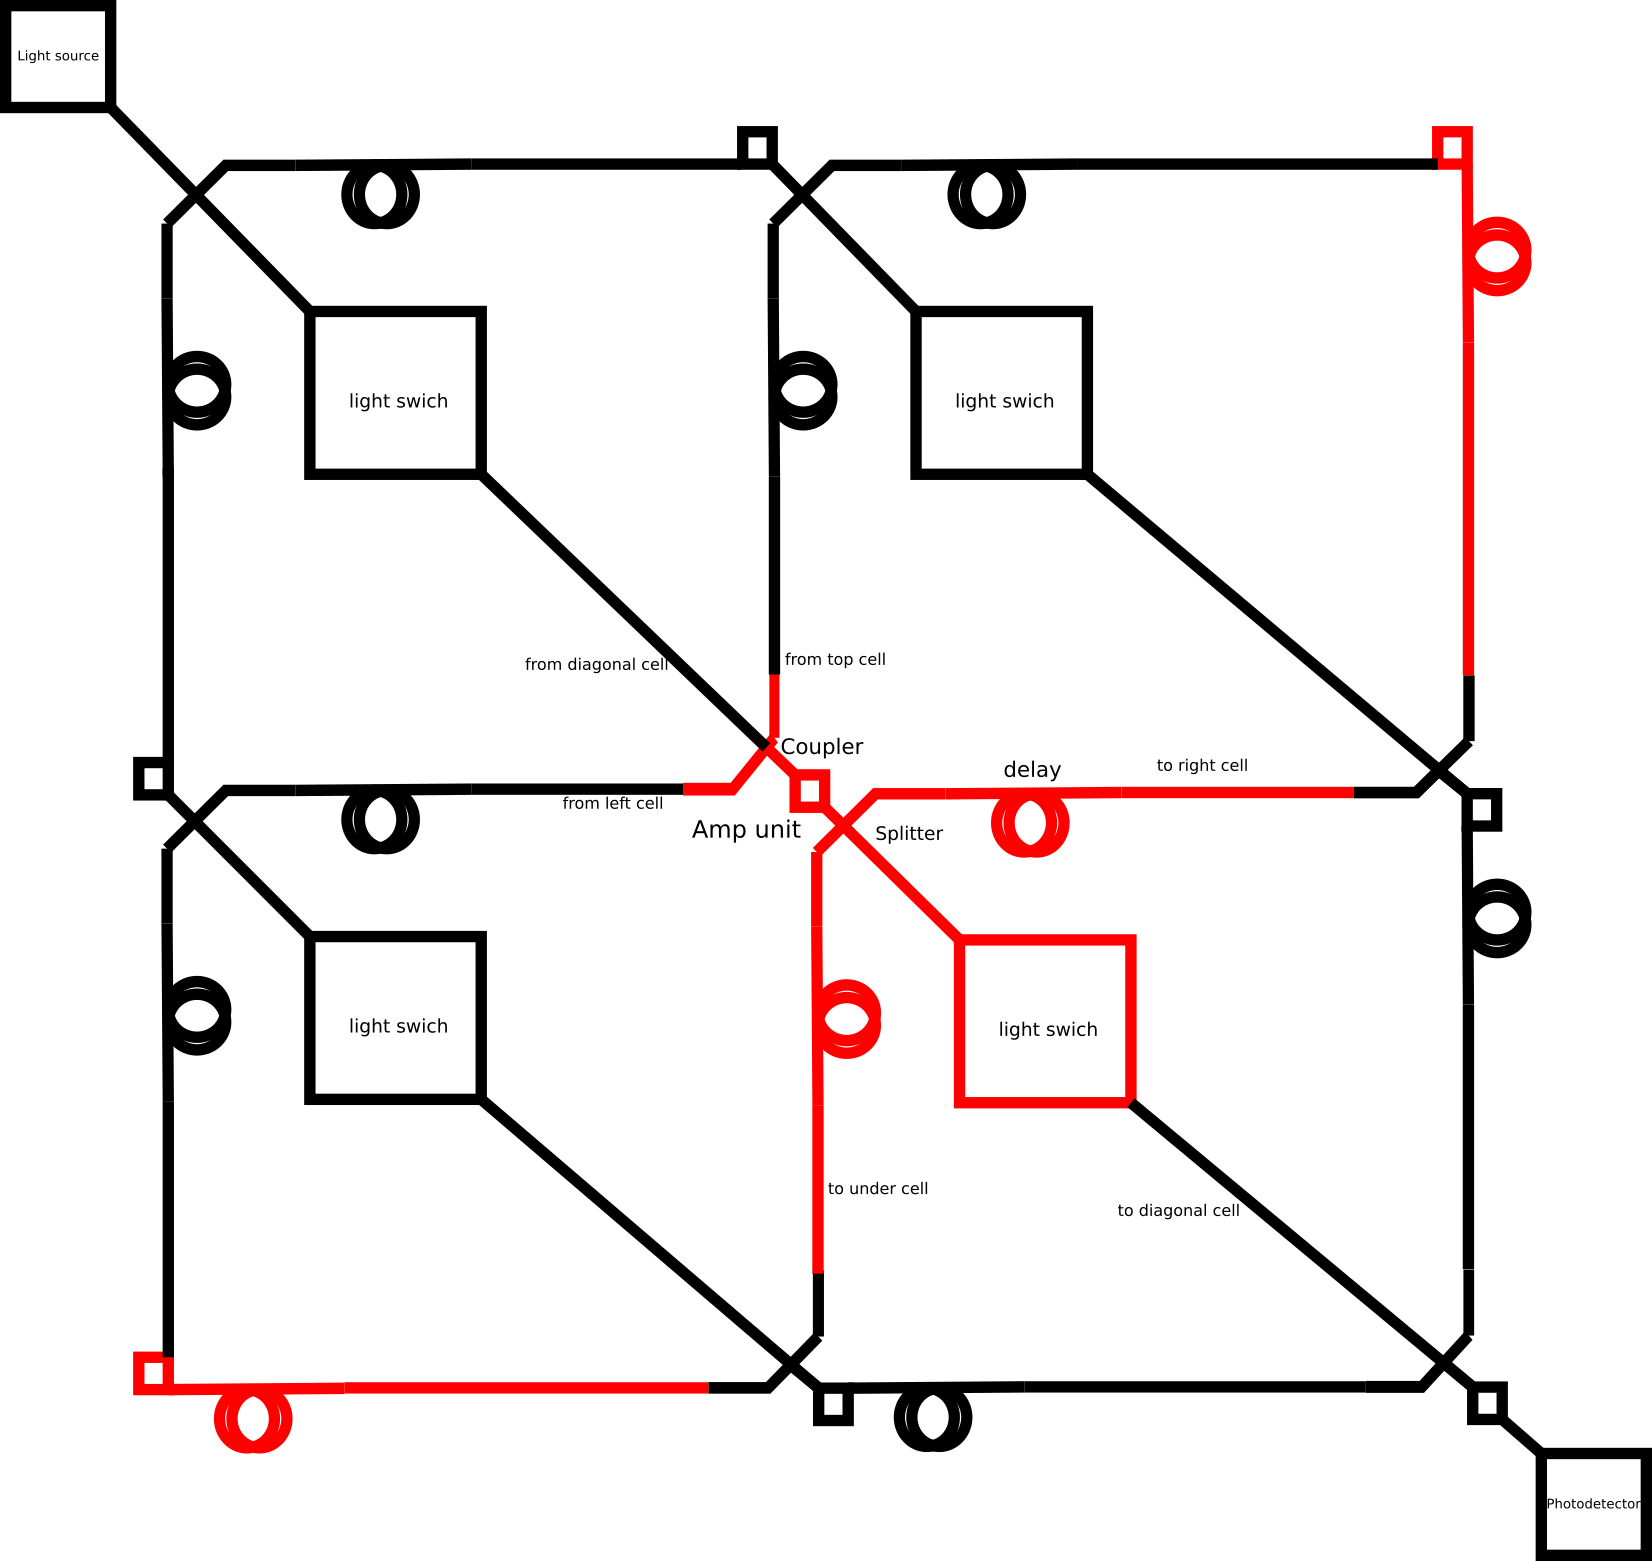
\includegraphics[keepaspectratio,scale=0.15]{fig/3/lightracelogic_N_2_off3.png}}
\subfigure[光伝搬信号入力から$4ns$後]{
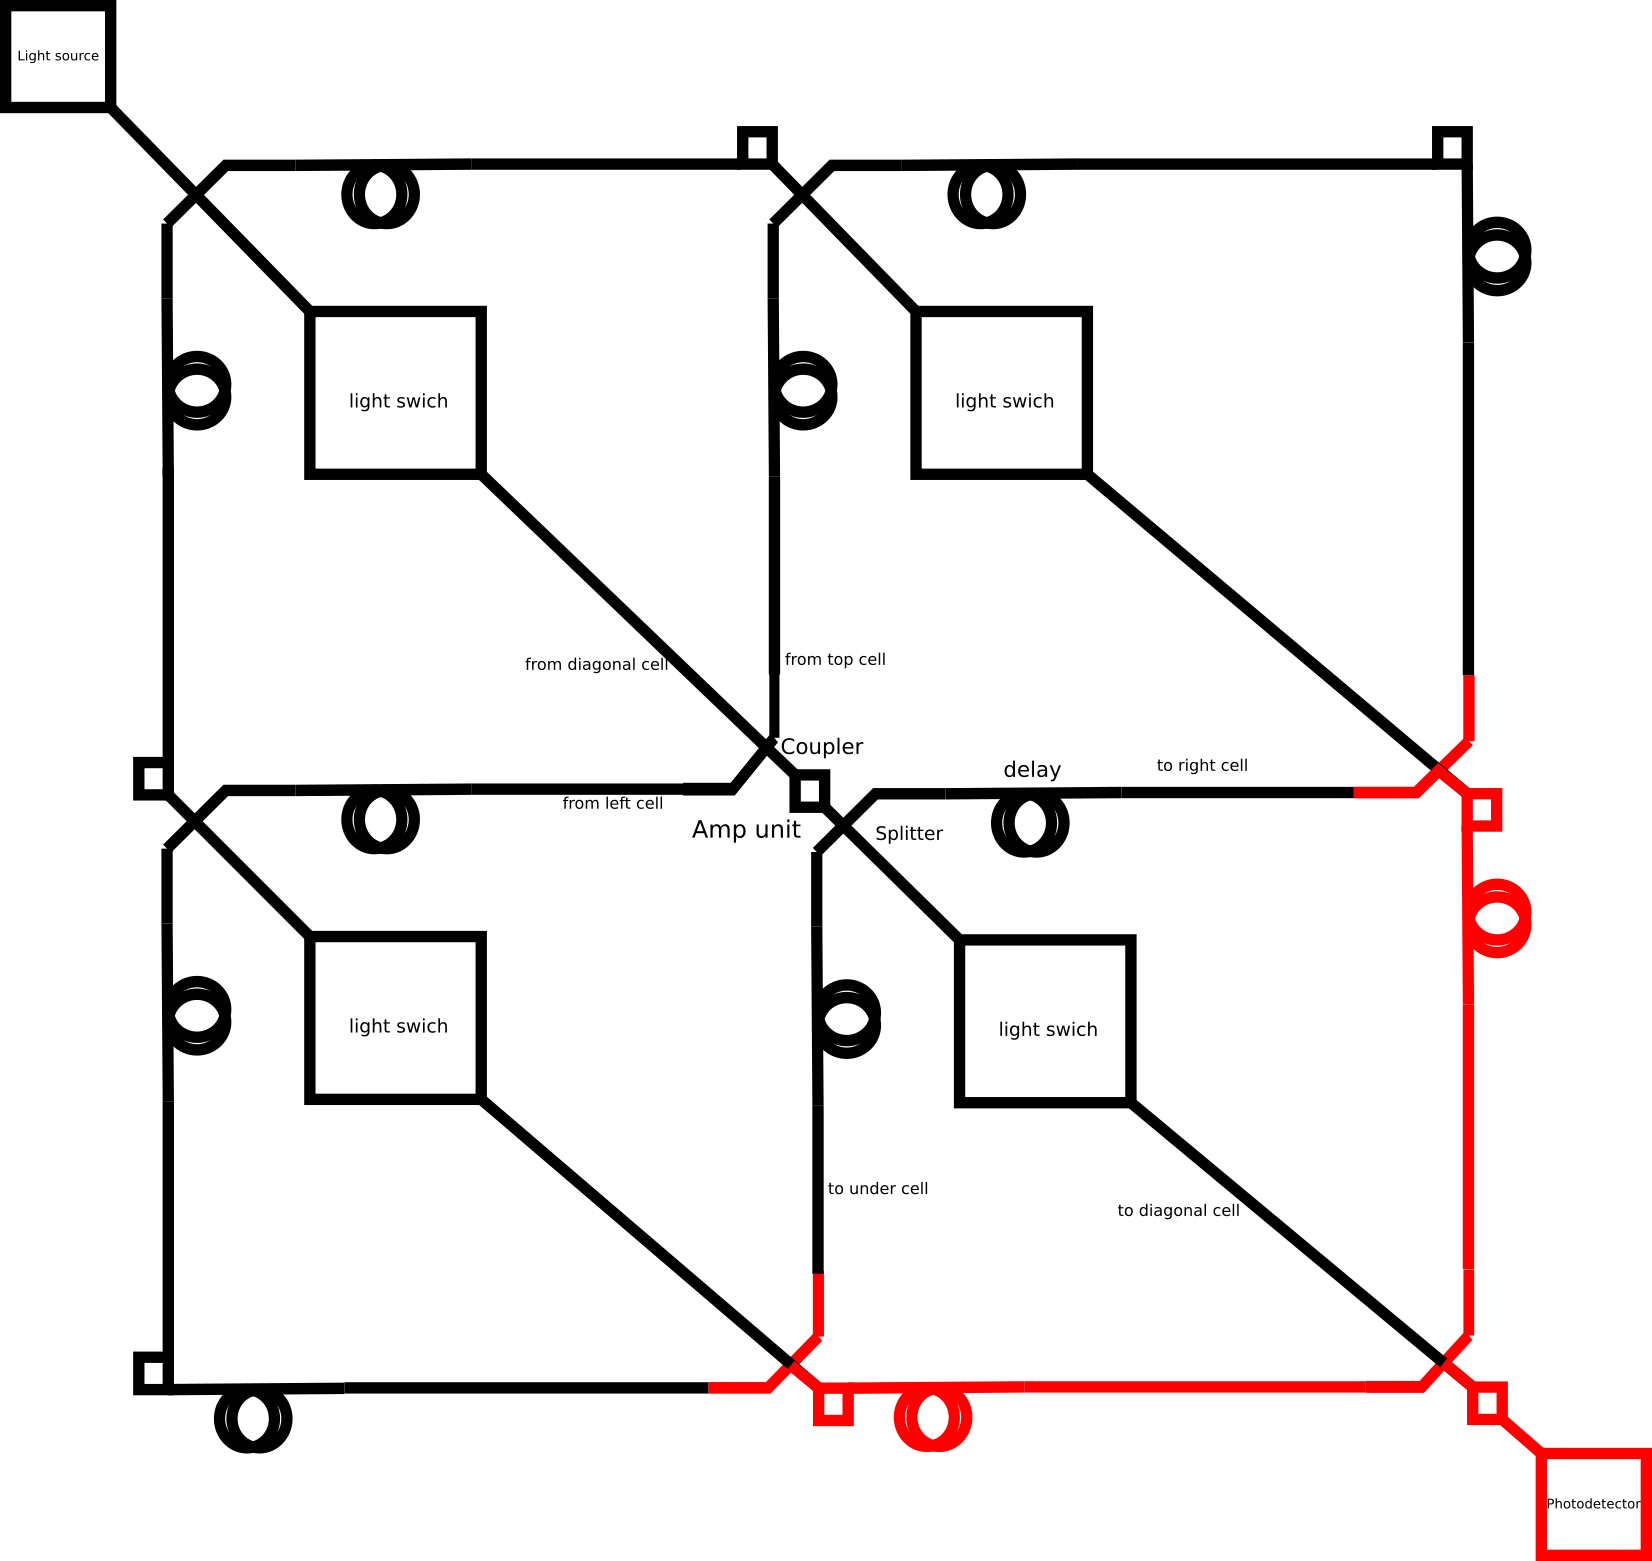
\includegraphics[keepaspectratio,scale=0.15]{fig/3/lightracelogic_N_2_off4.png}}\\
\caption{比較する文字列が完全に不一致の場合の光レースロジックアレイの挙動}
\label{fig:N=2_off}
\end{center}
\end{figure}


\chapter{検証・評価}
本章では提案したDNA配列アラインメントスコア計算用の光Race Logic回路について機能検証と評価を行う.
\section{検証}
検証に用いたのはOptiwave社が提供するOptisystemというシミュレータである.
OptiSystemは光ネットワークのあらゆるタイプの広範囲のシステムの設計,評価,シミュレーションを行なうソフトウェアである.
素子レベルからシステムレベルまでの物理レイヤー上の光通信システムの設計と解析を行うことができる.

配列長N=2のアラインメントスコアを求める提案回路について,光Race Logic arrayの動作を確認した.
今回のシミュレーションにおいて,各素子において光伝搬信号に影響を与える雑音や損失は考慮していない.
またOptisystemの仕様上,遅延素子で付与された遅延時間のみが考慮され,
素子や導波路の伝搬遅延については考慮されていない.
回路のスイッチが取りうる全状態を図\ref{fig:all_switch}に,
シミュレーションの結果を図\ref{fig:test}に示す.
今回のシミュレーションでは光遅延素子で発生する遅延時間が$1ns$と設定した.
\begin{figure}[t!]
\begin{center}
\subfigure[状態1]{
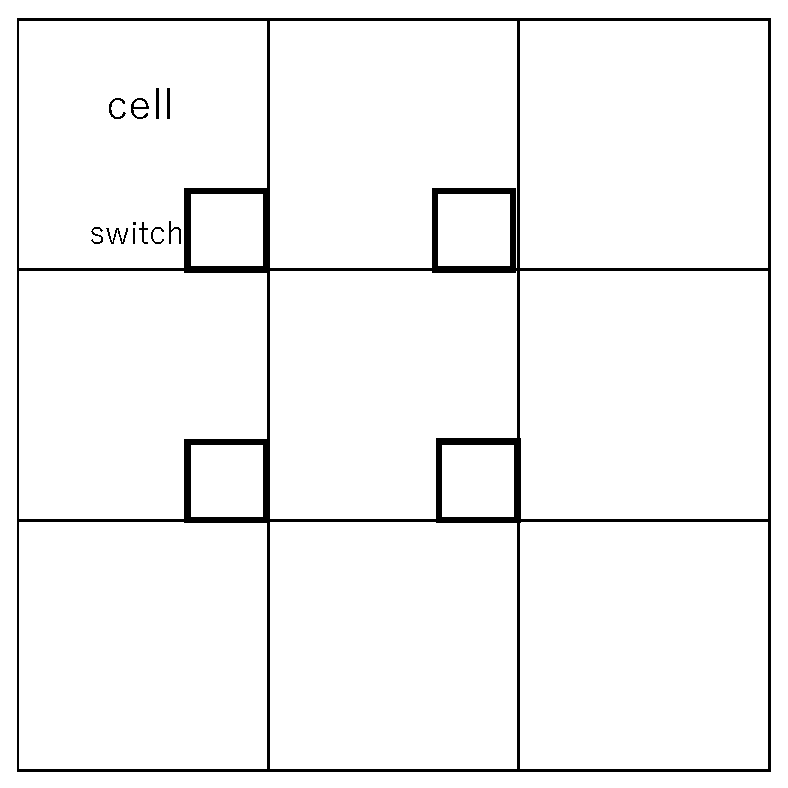
\includegraphics[keepaspectratio,scale=0.3]{fig/4/case1.eps}
\label{fig:all_switch_1}}
\subfigure[状態2]{
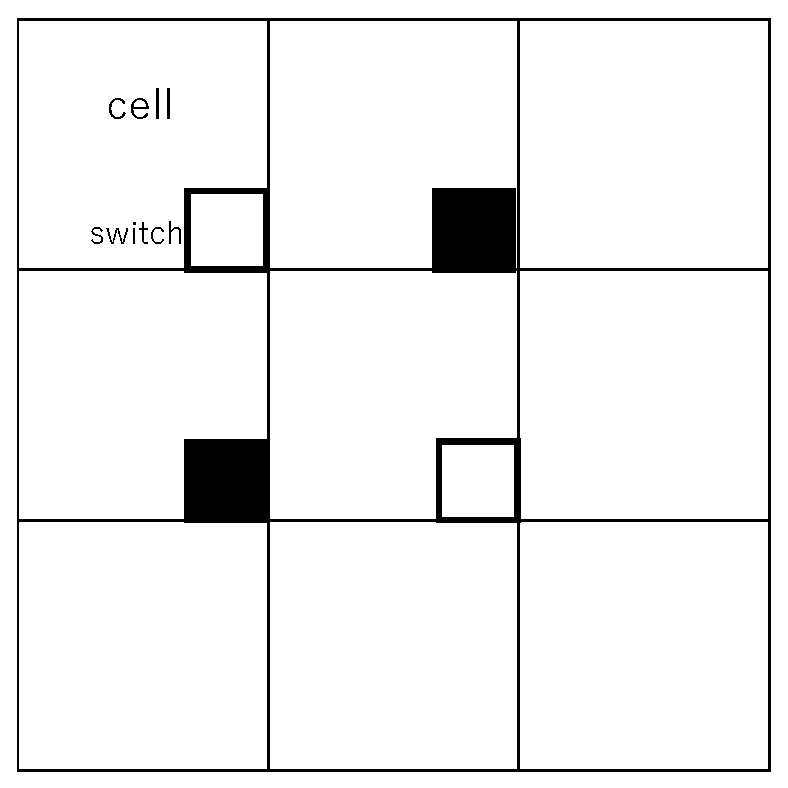
\includegraphics[keepaspectratio,scale=0.3]{fig/4/case2.eps}
\label{fig:all_switch_2}}
\subfigure[状態3]{
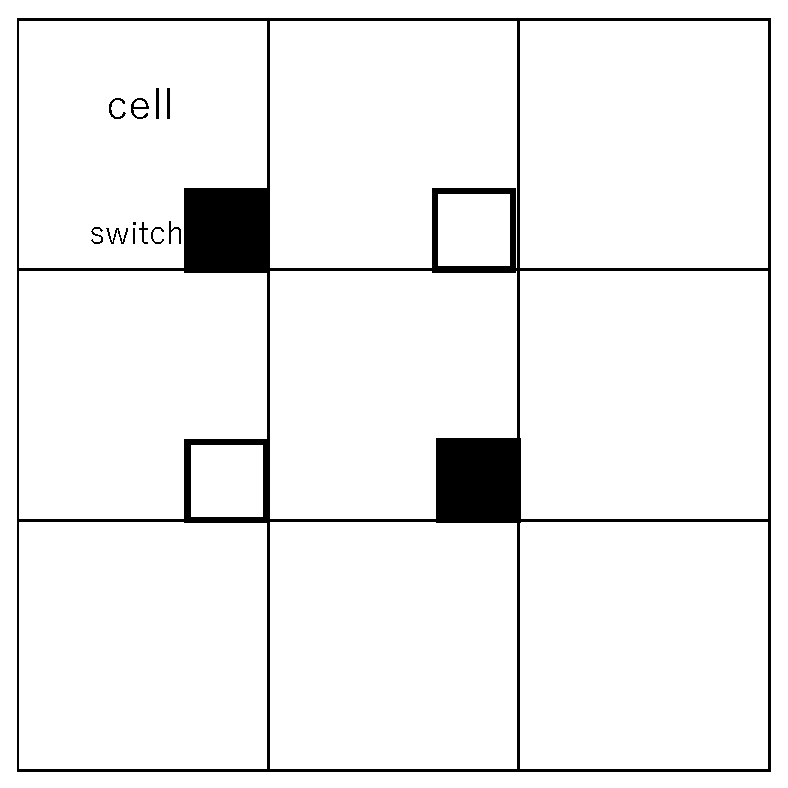
\includegraphics[keepaspectratio,scale=0.3]{fig/4/case3.eps}
\label{fig:all_switch_3}}\\
\subfigure[状態4]{
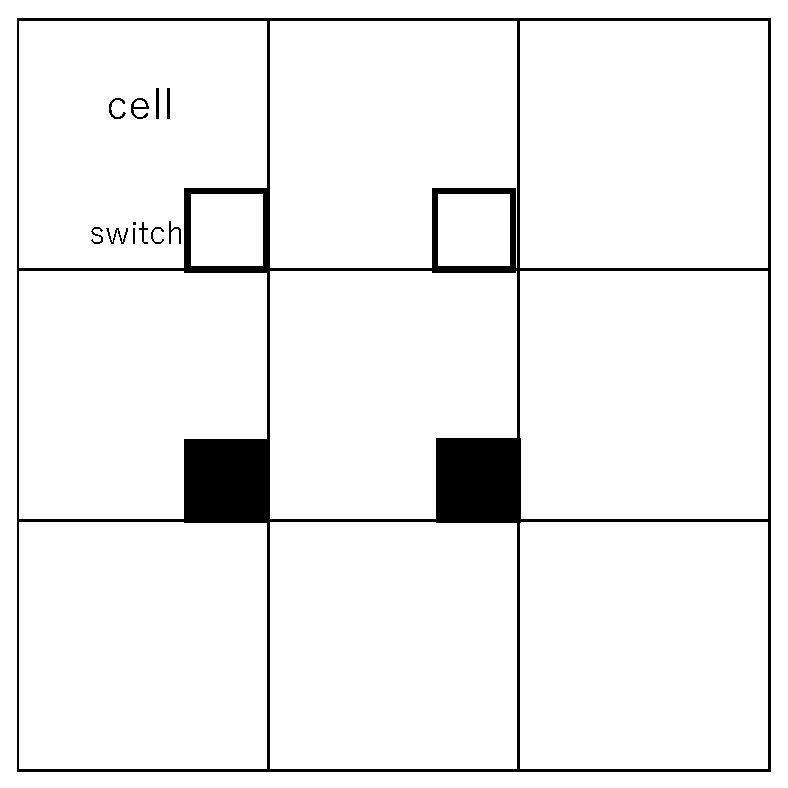
\includegraphics[keepaspectratio,scale=0.3]{fig/4/case4.eps}
\label{fig:all_switch_4}}
\subfigure[状態5]{
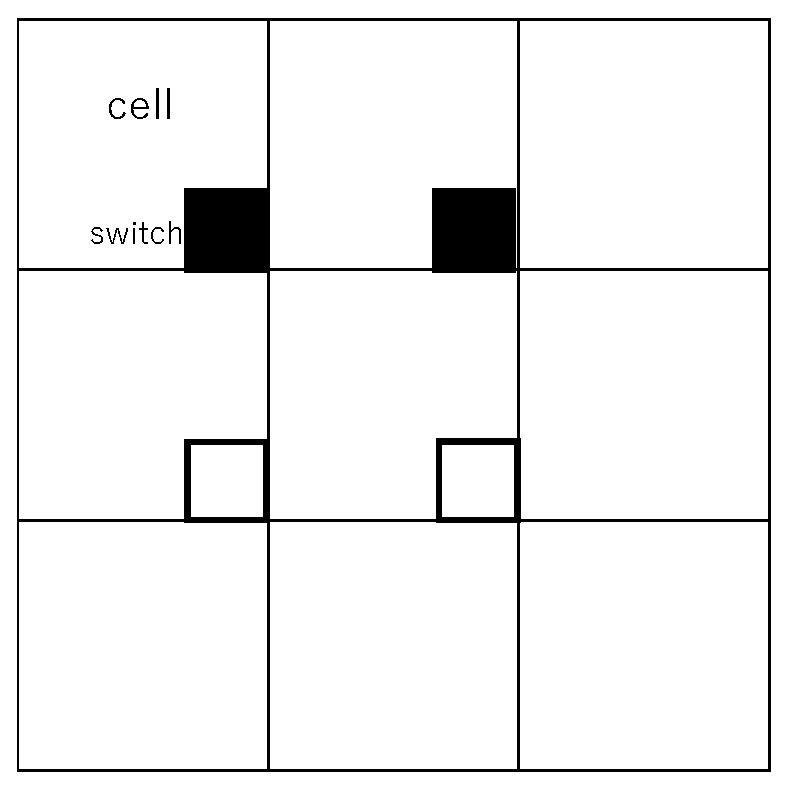
\includegraphics[keepaspectratio,scale=0.3]{fig/4/case5.eps}
\label{fig:all_switch_5}}
\subfigure[状態6]{
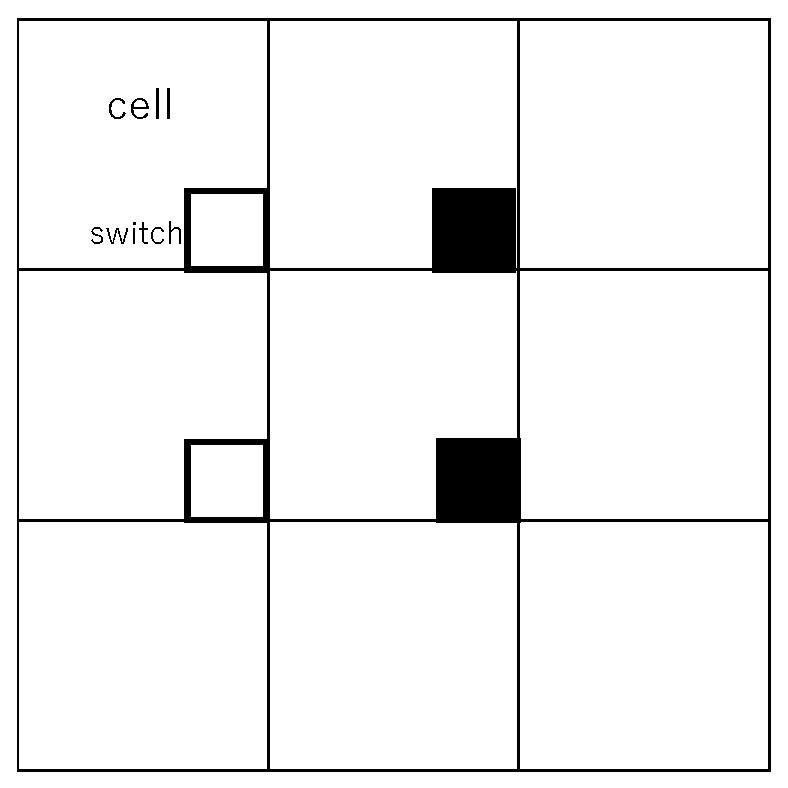
\includegraphics[keepaspectratio,scale=0.3]{fig/4/case6.eps}
\label{fig:all_switch_6}}\\
\subfigure[状態7]{
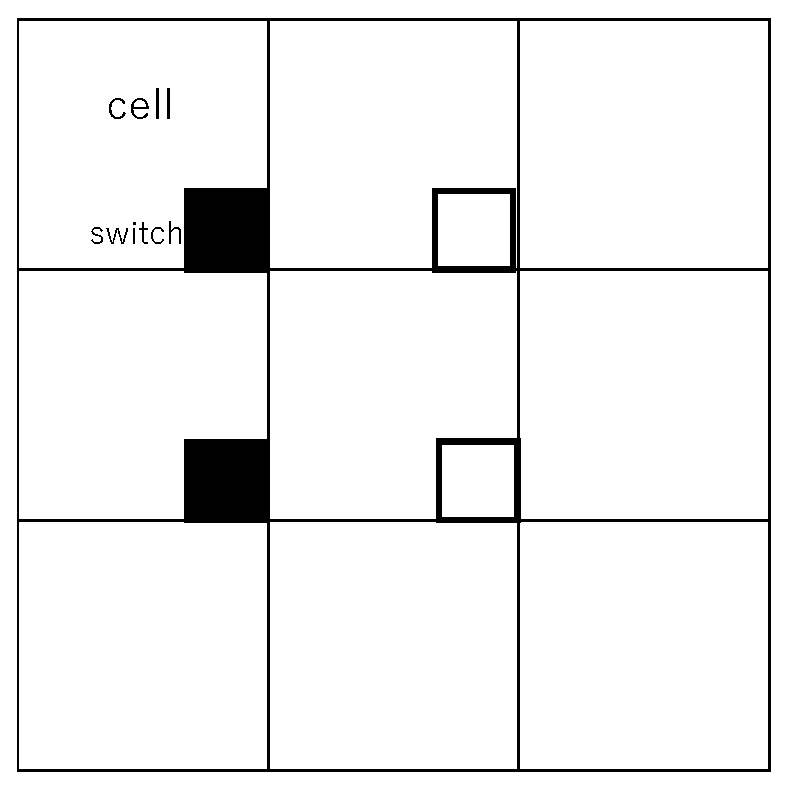
\includegraphics[keepaspectratio,scale=0.3]{fig/4/case7.eps}
\label{fig:all_switch_7}}
\subfigure[状態8]{
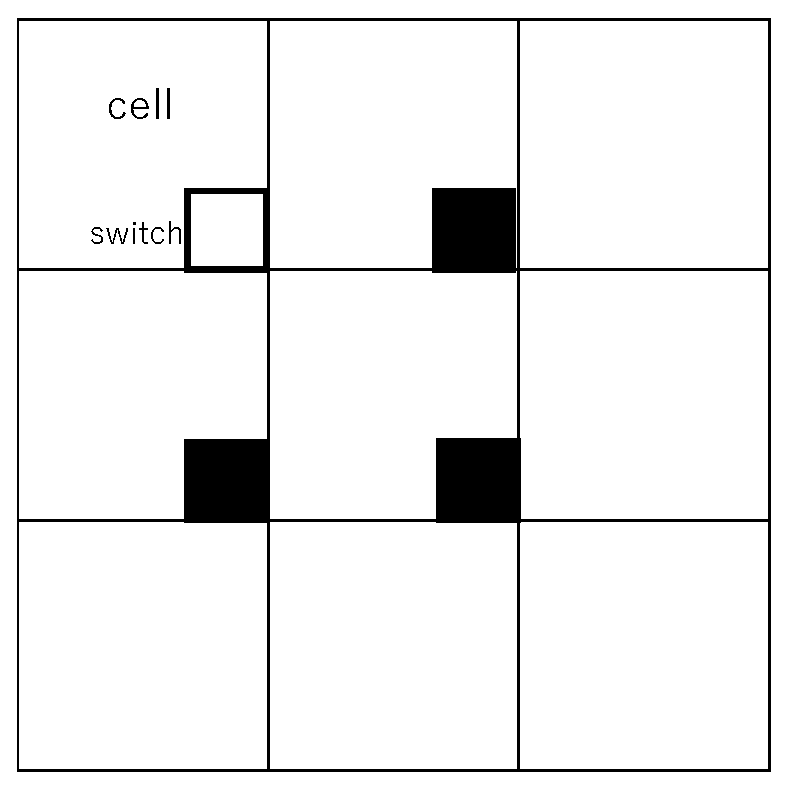
\includegraphics[keepaspectratio,scale=0.3]{fig/4/case8.eps}
\label{fig:all_switch_8}}
\subfigure[状態9]{
\includegraphics[keepaspectratio,scale=0.3]{fig/4/case9.eps}
\label{fig:all_switch_9}}\\
\subfigure[状態10]{
\includegraphics[keepaspectratio,scale=0.3]{fig/4/case10.eps}
\label{fig:all_switch_10}}
\subfigure[状態11]{
\includegraphics[keepaspectratio,scale=0.3]{fig/4/case11.eps}
\label{fig:all_switch_11}}
\subfigure[状態12]{
\includegraphics[keepaspectratio,scale=0.3]{fig/4/case12.eps}
\label{fig:all_switch_12}}\\
\caption{取りうる全スイッチの状態}
\label{fig:all_switch}
\end{center}
\end{figure}
\begin{figure}[t!]
\begin{center}
\subfigure[光Race Logic arrayへの光伝搬入力信号 1]{
\includegraphics[keepaspectratio,scale=0.23]{fig/4/test_in1.png}
\label{fig:test_in1}}
\subfigure[光Race Logic arrayへの光伝搬出力信号 1]{
\includegraphics[keepaspectratio,scale=0.23]{fig/4/test_out1.png}
\label{fig:test_out1}}\\
\subfigure[光Race Logic arrayへの光伝搬入力信号 2]{
\includegraphics[keepaspectratio,scale=0.23]{fig/4/test_in2.png}
\label{fig:test_in2}}
\subfigure[光Race Logic arrayへの光伝搬出力信号 2]{
\includegraphics[keepaspectratio,scale=0.23]{fig/4/test_out2.png}
\label{fig:test_out2}}\\
\subfigure[光Race Logic arrayへの光伝搬入力信号 3]{
\includegraphics[keepaspectratio,scale=0.23]{fig/4/test_in3.png}
\label{fig:test_in3}}
\subfigure[光Race Logic arrayへの光伝搬出力信号 3]{
\includegraphics[keepaspectratio,scale=0.23]{fig/4/test_out3.png}
\label{fig:test_out3}}
\caption{Optisystemでの光伝搬入出力信号}
\label{fig:test}
\end{center}
\end{figure}

表\ref{test_timing}に,図\ref{fig:all_switch}のそれぞれの状態ごとの,
\begin{enumerate}
\item 最初の光伝搬出力信号の伝搬遅延時間の想定値
\item シミュレータ上の回路のスイッチがその状態を取る区間
\item 結果から読み取った最初の光伝搬出力信号の伝搬遅延時間
\end{enumerate}
を示す.
\begin{table}[t!]
\begin{center}
\caption{配列長N=2の光Race Logic arrayの動作検証結果}
\begin{tabular}{|c|c|c|c|} \hline
&1&2&3\\ \hline \hline
状態1&$2ns$&図\ref{fig:test_in1},\ref{fig:test_out1}の$ns〜ns区間$&$2ns$\\ \hline
状態2&$2ns$&図\ref{fig:test_in1},\ref{fig:test_out1}の$ns〜ns区間$&$2ns$\\ \hline
状態3&$3ns$&図\ref{fig:test_in1},\ref{fig:test_out1}の$ns〜ns区間$&$3ns$\\ \hline
状態4&$3ns$&図\ref{fig:test_in1},\ref{fig:test_out1}の$ns〜ns区間$&$3ns$\\ \hline
状態5&$3ns$&図\ref{fig:test_in2},\ref{fig:test_out2}の$ns〜ns区間$&$3ns$\\ \hline
状態6&$3ns$&図\ref{fig:test_in2},\ref{fig:test_out2}の$ns〜ns区間$&$3ns$\\ \hline
状態7&$3ns$&図\ref{fig:test_in2},\ref{fig:test_out2}の$ns〜ns区間$&$3ns$\\ \hline
状態8&$3ns$&図\ref{fig:test_in2},\ref{fig:test_out2}の$ns〜ns区間$&$3ns$\\ \hline
状態9&$3ns$&図\ref{fig:test_in3},\ref{fig:test_out3}の$ns〜ns区間$&$3ns$\\ \hline
状態10&$3ns$&図\ref{fig:test_in3},\ref{fig:test_out3}の$ns〜ns区間$&$3ns$\\ \hline
状態11&$3ns$&図\ref{fig:test_in3},\ref{fig:test_out3}の$ns〜ns区間$&$3ns$\\ \hline
状態12&$4ns$&図\ref{fig:test_in3},\ref{fig:test_out3}の$ns〜ns区間$&$4ns$\\ \hline
\end{tabular}
\label{test_timing}
\end{center}
\end{table}

この機能検証結果から,光Race Logic arrayが
想定した動作をしていることが確認できた.

\section{評価}
本節では,提案した光Race Logic arrayが
一組の配列のアラインメントを求める(以後,これを一計算と呼称する)ために必要な
遅延時間や面積及び消費電力が
配列長Nによってどう変化するかを見積るために
各項目を算出するモデル式を構築し,評価を行う.

\subsection{遅延時間}
光Race Logic arrayに光伝搬信号が入射されてからarray内を伝搬し,
最初に出力された信号が受光器で検出されるまでの遅延時間を考える.
配列長Nの光Race logic arrayにおいて,最初に光伝搬信号が出力されるまでの回路遅延時間は
配列の組み合わせによって異なる.
二つの配列が完全に不一致の場合,最初に光伝搬信号が出力されるまでの回路遅延時間は
最長となる.
今回はこのワーストケースの遅延時間をモデル化した.

図\ref{fig:proposalcell}の構造より構築した遅延時間$T$のモデル式を式\ref{eq:latency}に示す.
\begin{eqnarray}
&&T = T_{wire}+2N \times T_{cell-pass}+T_{pd} \nonumber \\
&&T_{cell-pass} = T_{cell-wire}+T_{coupler}+T_{amp}+T_{splitter}+T_{switch-pass}
\label{eq:latency}
\end{eqnarray}

$T_{wire}はセル間の配線遅延時間,T_{cell-pass}は一つのセルを通過する遅延時間,T_{pd}は受光器の応答時間である.$
$T_{cell-pass}の内訳はT_{cell-wire}がセル内部の配線遅延,$
$T_{coupler}・T_{splitter}がそれぞれ光結合器・光分配器の遅延時間,$
$T_{amp}がアンプの遅延時間,T_{switch-pass}が光スイッチ遅延時間である.$
$T_{wire}とT_{cell-pass}が光伝搬入力信号が$光Race Logic array$を伝搬するために必要な時間,$
$T_{pd}が受光器が光出力信号を検出するまでに必要な時間である.$
式\ref{eq:latency}に示す通り,遅延時間は
配列長Nに線形にスケーリングする.

光伝搬信号は光デバイス内部を光速で通過するため,光デバイス内の遅延時間は素子のゲート長に依存する.
今回は,ナノフォトニック・デバイスのゲート長が100,10,1$\mu m$の場合の
光Race Logic arrayの遅延時間を示す.
なお,配線遅延に関しては今回は無視している.
図\ref{fig:nanolatency}の縦軸は遅延時間,横軸は配列長Nである.
図\ref{fig:nanolatency}より,ナノフォトニック・デバイスのゲート長が小さいほど
遅延時間が小さくなることが読み取れる.
\begin{figure}[t!]
\begin{center}
\includegraphics[keepaspectratio,scale=0.5]{fig/4/nanolatency.png}
\caption{光Race Logic arrayの遅延時間}
\label{fig:nanolatency}
\end{center}
\end{figure}

\subsection{面積}
提案したセルの構成(図\ref{fig:proposalcell})より,
セル一つの面積$A_{cell}$を表すモデル式は式\ref{eq:cellArea}と書ける.
\begin{equation}
A_{cell} = A_{cell-wire}+A_{coupler}+A_{amp}+A_{splitter}+A_{switch}+2A_{delay}
\label{eq:cellArea}
\end{equation}

$A_{cell-wire}はセル内部の配線面積,A_{amp}がアンプの面積,$
$A_{coupler}・A_{splitter}はそれぞれ光結合器・光分配器の遅延時間,$
$A_{switch}が光スイッチの面積,A_{delay}は光遅延素子の面積である.$
このセルを基準セルとする.

セルを並べてarrayを構成した時に,外周のセルはこの基準セルとは違う構成となる.
その差異の理解を助けるため,図\ref{fig:N=2}に配列長N=2の光Race Logic arrayの構造を示す.
\begin{figure}[t!]
\begin{center}
\includegraphics[keepaspectratio,scale=0.35]{fig/4/lightracelogic_N_2.png}
\caption{配列長N=2の光Race Logic arrayの構造}
\label{fig:N=2}
\end{center}
\end{figure}

この差異に留意しながら,配列長Nの光Race logic arrayの面積$A$をモデル化した.
モデル式を式\ref{eq:Area}に示す.
\begin{equation}
A = A_{wire}+N^2 \times A_{cell} + 2N \times (A_{delay}+A_{amp}) +A{ls}+A_{pd}
\label{eq:Area}
\end{equation}

$A_{wire}はセル間の配線面積,A{ls}は光源の面積,A_{pd}は受光器の面積である.$
式\ref{eq:Area}が示すように,面積は
配列長Nの2乗にスケーリングする.

ナノフォトニック・デバイスのゲート長が100,10,1$\mu m$の場合の
光Race Logic arrayの面積を示す.
なお,配線面積に関しては今回は無視している.
図\ref{fig:nanoArea}の縦軸は光Race Logic arrayの面積,横軸は配列長Nである.
\begin{figure}[t!]
\begin{center}
\includegraphics[keepaspectratio,scale=0.5]{fig/4/nanoArea.png}
\caption{光Race Logic arrayの面積}
\label{fig:nanoArea}
\end{center}
\end{figure}

\subsection{消費電力}
ここで本提案の光Race Logic arrayでの消費電力について考える.
この回路での消費電力は,式\ref{eq:power}に示すように
$光源の消費電力P_{ls}$,$アンプP_{amp}$の消費電力の二つのみで考えることができる.
\begin{equation}
P=P_{ls}+P_{amp}
\label{eq:power}
\end{equation}

$P$の値は,光Race Logic arrayが機能を担保できる値に設定しなければならない.
そこで,光Race Logic arrayの機能担保について具体的に見ていく.

配列長Nの光Race Logic arrayのN行N列目のセルからの
光伝搬出力信号強度$P_{out\,N,N}$は
式\ref{eq:power_out}と表せる.
\begin{equation}
P_{out\,N,N}=Loss_{N,N}(P_{out\,(N-1),(N-1)}+P_{out\,(N-1),N}+P_{out\,N,(N-1)})
\label{eq:power_out}
\end{equation}

$N \geq 0,P_{out\,-1,-1}=P_{ls},P_{out\,-1,0}=0,P_{out\,0,-1}=0である.$
$Loss_{N,N}$はN行N列目のセルに光伝搬信号が入力されてから出力される際のロスである.

$P_{out\,N,N}$の値は配列の組み合わせ,即ちスイッチの状態によって大きく変化する.
光Race Logic arrayからの光伝搬出力信号は受光器で検出されなければならない.
受光器の最小受光感度$P_{r}$を用いると,
$P_{out\,N,N}の最小値 \geq P_{r}となるようにP$の値を決定することが必要となる.

\subsubsection{ケーススタディ:配列長N=2の光Race logic arrayにおける消費電力}
ここで,図\ref{fig:loss}に示すように各素子における損失が一律で$\alpha$の場合において,
配列長N=2の光Race logic arrayにおける消費電力を考える.
\begin{figure}[t!]
\begin{center}
\includegraphics[keepaspectratio,scale=0.5]{fig/4/loss.eps}
\caption{光素子における損失例}
\label{fig:loss}
\end{center}
\end{figure}
この$\alpha$は0〜1の範囲の値を取る.
図\ref{fig:proposalcell}に示すセルにおいて,光信号を伝搬させる際に損失を与える素子は
光結合器,光分配器,光スイッチ,光遅延素子とする.
この4つの素子での損失を$\alpha$とし,その他の損失は考えない.
今回は回路規模が小さいので,各セルのアンプユニットでの
光伝搬信号強度の増幅は行わず,
光源の光出力信号強度を変えることによって$P_{out\,N,N}の最小値 \geq P_{r}となるように$する.
この光Race logic arrayの消費電力$PはP=P_{ls}$となる.

配列長N=2の光Race logic arrayの光スイッチは,配列の組み合わせによってその状態を変え,
図\ref{fig:all_switch}に示す12通りのいずれかの状態を取る.
図\ref{fig:all_switch}中のスイッチは,白塗りがONの状態を,
黒塗りがOFFの状態をそれぞれ表している.
図\ref{fig:all_switch_1}〜図\ref{fig:all_switch_2}は配列が完全に一致する場合,
図\ref{fig:all_switch_3}〜図\ref{fig:all_switch_11}は配列中1文字がする場合,
図\ref{fig:all_switch_12}は配列が完全に不一致の場合である.
各状態での出力を以下に示す.
\begin{itemize}
\item 状態1(図\ref{fig:all_switch_1})の出力 $P_{out\,2,2}=P_{ls}\frac{(1-\alpha)^6}{3^2}$\\
\item 状態2(図\ref{fig:all_switch_2})の出力 $P_{out\,2,2}=P_{ls}\frac{(1-\alpha)^6}{3^2}$\\
\item 状態3(図\ref{fig:all_switch_3})の出力 $P_{out\,2,2}=P_{ls}\frac{2(1-\alpha)^7}{3^2}$\\
\item 状態4(図\ref{fig:all_switch_4})の出力 $P_{out\,2,2}=P_{ls}\frac{(1-\alpha)^7\bigl\{2(1-\alpha)+1\bigl\}}{3^2}$\\
\item 状態5(図\ref{fig:all_switch_5})の出力 $P_{out\,2,2}=P_{ls}\frac{(1-\alpha)^7\bigl\{\frac{2}{3}(1-\alpha)+1\bigl\}}{3^2}$\\
\item 状態6(図\ref{fig:all_switch_6})の出力 $P_{out\,2,2}=P_{ls}\frac{(1-\alpha)^7\bigl\{2(1-\alpha)+1\bigl\}}{3^2}$\\
\item 状態7(図\ref{fig:all_switch_7})の出力 $P_{out\,2,2}=P_{ls}\frac{(1-\alpha)^7\bigl\{\frac{2}{3}(1-\alpha)+1\bigl\}}{3^2}$\\
\item 状態8(図\ref{fig:all_switch_8})の出力 $P_{out\,2,2}=P_{ls}\frac{2(1-\alpha)^8}{3^2}$\\
\item 状態9(図\ref{fig:all_switch_9})の出力 $P_{out\,2,2}=P_{ls}\frac{(1-\alpha)^7}{3^2}$\\
\item 状態10(図\ref{fig:all_switch_10})の出力 $P_{out\,2,2}=P_{ls}\frac{(1-\alpha)^7}{3^2}$\\
\item 状態11(図\ref{fig:all_switch_11})の出力 $P_{out\,2,2}=P_{ls}\frac{2(1-\alpha)^8}{3^3}$\\
\item 状態12(図\ref{fig:all_switch_12})の出力 $P_{out\,2,2}=P_{ls}\frac{2(1-\alpha)^8\bigl\{\frac{2}{3}(1-\alpha)^2+1\bigl\}}{3^2}$\\
\end{itemize}

以上のスイッチ状態の中で,その出力強度が最小となるのは状態11(図\ref{fig:all_switch_11})の場合である.
よって,各素子における損失が一律で$\alpha$の
配列長N=2の光Race logic arrayでは,
$P_{ls}\frac{2(1-\alpha)^8}{3^3} \geq P_{r}$となるように$P_{ls}$の値を決定する必要がある.
受光器の最小受光感度を$P_{r}=-20[dBm]=0.01[mW]$,$\alpha = $0.1,0.01の場合の$P_{ls}$を表\ref{pls}に示す.
\begin{table}[t!]
\begin{center}
\caption{配列長N=2の光Race logic arrayの消費電力}
\begin{tabular}{|c|c|c|} \hline
&$\alpha = $0.1&$\alpha = $0.01\\ \hline \hline
$P_{ls}[mW]$&0.314&0.144\\ \hline
\end{tabular}
\label{pls}
\end{center}
\end{table}

\chapter{おわりに}

ナノフォトニクスと呼ばれる新しい光素子技術と
このナノフォトニクスを用いて機能を実現したナノフォトニック・デバイスが
光速度で演算を実現できる素子として注目されている.
本研究ではRace Logicと光デバイスとの親和性に着目し,
ナノフォトニック・デバイスを用いたアーキテクチャ検討の一環として
光Race Logic arrayを提案した.
また,遅延時間・面積・消費電力についてのモデリングを行い,
配列長Nによって
それぞれの項目がどう変化するのかを示した.
遅延時間はNに線形に従い,面積はNの2乗に従うことが分かった.
消費電力に関しては,ケーススタディとしてN=2の場合の値を示した.

光Race Logic回路の性能を律速する要因として遅延時間差を検知する
部分の構造が重要になることを考察した.
検知部分は重み付けに用いる遅延時間の最小単位を検知できなければいけない.
ゲート長によって遅延時間が決定する光デバイスにおいて
ゲート長を1$\mu m$のサイズで加工するとき,
重み付けに用いる遅延時間の最小単位は10$fs$になる.
この遅延時間の最小単位を計測することができる検知部分の構成を考える必要がある.

また,光伝搬信号の強度や遅延時間に影響を与える雑音が
光Race Logic arrayの規模を律速しうると考察した.
雑音が光Race Logic arrayの規模を具体的にどう律速するのかを考えていかなければならない.

更に,出力信号の遅延時間に情報を付与するRace Logicの考えを発展させ,
光出力信号の位相や強度に情報を付与できる可能性も見えてきた.
光デバイス独自の設計選択肢が存在するのである.

ナノフォトニック・デバイスを用いた光Race Logic回路の実現に向けて,
雑音の影響を具体的に示すことと設計選択肢ごとの検知部分の構成が今後の課題である.



\acknowledgment
本研究の進行および本論文執筆にあたりまして,懇切丁寧なご指導を頂きました井上弘士教授に心より感謝申し上げます.本論文執筆にあたり,多大なご指導を頂きました小野貴継助教に心より感謝申し上げます.
本研究を行うにあたり,多大なご指導を賜りました日本電信電話株式会社\ 物性科学基礎研究所\ ナノフォトニクスセンタ\ 主幹研究員\ 新家昭彦様に感謝の意を表するとともに厚く御礼申し上げます.
本論文執筆にあたり多大な指導頂きました,井上研究室大学院博士2年川上哲志氏に深く感謝致します.

最後に,井上研究室の皆様の御意見,御厚意に感謝の意を表します.

%\appendix

\bibliographystyle{junsrt}
\bibliography{grad}


\end{document}
